% rubber: setlist arguments --shell-escape
\documentclass[lablogo]{thesis}


\title{Secure Security at the Security-Critical Interface}
\author{Atri Bhattacharyya}
\president{Prof. Professor Mc. ProfessorFace}
\director{Prof. Mathias Payer}
\codirector{Prof. Babak Falsafi}
\internal{Prof. Professor Mc. ProfessorFace}
\external{Prof. Professor Mc. ProfessorFace}
\external{Dr. Anil Kurmus}

\cv{Resume.pdf}

%%%%%%%%%%%%% Standard list of used packages %%%%%%%%%%%%%%%%
% \usepackage{cite}
\usepackage{amsmath,amsfonts}
% \usepackage{amssymb, amsfonts}
\usepackage{graphicx}
\usepackage{textcomp}
\usepackage{xcolor}
\usepackage{fancyhdr}
\usepackage{booktabs}
% \usepackage[hyphens]{url}
\usepackage[mathscr]{euscript}

% \usepackage[normalem]{ulem}

% Atri's list of typically used packages
% List of unused packages from Midas/TikTok
\usepackage{adjustbox}
% \usepackage{amsmath}
% \usepackage{filecontents}
% \usepackage{tikz}
\usepackage{xspace}
\usepackage{listings}
% \usepackage{xcolor}
% \usepackage{textcomp}
% \usepackage{graphicx}
% \usepackage{caption}
% \usepackage{subcaption}
% \usepackage{todonotes}
\usepackage{multirow}
\usepackage{multicol}
% \usepackage{booktabs}
\usepackage{paralist}       % For inparaenum
% \usepackage{enumitem}
% \usepackage{tabulary}
% \usepackage{verbatim}
\usepackage{balance}
\usepackage{tabularx}
\usepackage{algorithm}
\usepackage{algpseudocode}
\usepackage{braket}         % Fancy brackets
\usepackage{threeparttable} % Table with footnotes
\usepackage{makecell}       % Fancy multiline cells in table
\usepackage{pifont}         % For fancy dingbats, example xmark
\usepackage{comment}        % For comment environment
\usepackage{prettyref}    % For labels for autoref
% \usepackage[bookmarks=true,breaklinks=true,letterpaper=true,colorlinks,linkcolor=black,citecolor=blue,urlcolor=black]{hyperref}
                            % For autoref
\usepackage{listofitems}    % For `readlist` used for \newreviewer command
\usepackage{soul}           % For strikethrough \st


%%%%%%%%%% Sid's list of packages %%%%%%%%%%
% \usepackage[normalem]{ulem}
% \usepackage[final]{microtype}
% \usepackage[keeplastbox]{flushend}
% \usepackage{soul}
% \usepackage{makecell}
% \usepackage{hyphenat}
% \usepackage{subfig}
% \usepackage{color}
% \usepackage{balance}    
% \usepackage{verbatimbox}
% \usepackage{fancyvrb}
% \usepackage{enumitem}

%%%%%%%%%% Packages borrowed from Ahmad's thesis %%%%%%%%%%%%%%%%%%
% \usepackage{titlesec}
% \titleformat{\chapter}[display]
%   {\normalfont\huge\bfseries}{\chaptertitlename\ \thechapter}{20pt}{\Huge}
% \titlespacing*{\chapter}{0pt}{-20pt}{40pt}

% \usepackage{xcolor}
% \usepackage{xspace}
\usepackage{epigraph}
% \usepackage{enumitem}                 % custom lists
% \usepackage{listings}                 % code formatting
% \usepackage{tikz}
% \usepackage{expl3}
% \usepackage{caption}                  % figure captioning
% \usepackage{subcaption}               % subfigures
% \usepackage{listofitems}              % \readlist
% \usepackage{fontawesome}              % faArrowUp, etc...
% \usepackage{siunitx}                  % \num, SI units
% \usepackage{xpatch}                   % \xapptocmd
% \usepackage{minted}                   % listing environment (TODO replace with consistent code listings)
% \usepackage{algorithm}                % algorithm environment
% \usepackage{algpseudocode}            % \algnewcommand, \Procedure, \Call, etc...
% \usepackage{varwidth}                 % varwidth environment
% \usepackage{fmtcount}                 % \numberstringnum
% \usepackage{refcount}                 % \getrefnumber
% \usepackage{soul}                     % \sethlcolor
% \usepackage{adjustbox}                % adjustbox environment
% \usepackage{booktabs}                 % \toprule
% \usepackage{multirow}                 % \multirow
% \usepackage{colortbl}                 % \cellcolor
% \usepackage{pifont}                   % \ding
% \usepackage{makecell}                 % \multirowcell
% \usepackage{rotating}                 % sideways environment
% \usepackage{pgfplots}                 % axis environment
% \usepackage{csquotes}                 % \enquote
% % \usepackage{annotate-equations}
% \usepackage{bbding}                   % \XSolidBold
% \usepackage{ifsym}                    % \textifsymbol
% \usepackage{nicefrac}                 % \nicefrac
% % \usepackage{amsmath}
% \usepackage{amssymb}                  % \npreceq etc...
% \usepackage{pgf-umlsd}                % sequencediagram environment
% \usepackage{tikz-layers}
% \usepackage{scalerel}
% \usepackage{graphicx}
% \usepackage{threeparttable} % Table with footnotes
% \usepackage[
%   backend=bibtex,
%   style=numeric-comp,
%   hyperref=true,
%   defernumbers=true,
%   maxbibnames=99,
%   maxcitenames=1
% ]{biblatex}
% \addbibresource{thesis.bib}

%%%%%%%%%%%%%%%%%%%%% Commenter's sections %%%%%%%%%%%%%%%%%%%%%%%
% Enable or disable reviews
\newif\ifreview
% \reviewtrue   % comment this line to disable reviews
% newreviewer command description
\newcounter{ReviewerID}
\readlist*\annotationcolors{blue, red, orange, green, purple, yellow, brown, olive}
\newcommand{\newreviewer}[2]{%
  \ifnum \theReviewerID=\annotationcolorslen
    \setcounter{ReviewerID}{0} % cycle through colors
  \fi
  \stepcounter{ReviewerID}%
  \expandafter\edef\csname bootstrap#1\endcsname{%
    \expandafter\def\csname #1\endcsname####1{%
      \ifreview%
        {\noexpand\color{\annotationcolors[\theReviewerID]} {\noexpand\bf{\noexpand\fbox{#2}} {\noexpand\it ####1} }}
      \else%
        {}% disable annotations
      \fi%
    }%
  }%
  \csname bootstrap#1\endcsname%
}
% List of reviewers
% Command: \newreviewer{latexcommand}{visiblename}
% You will be able to use a command \latexcommand{comment}
% to generate a colored comment prepended by visiblename.
\newreviewer{mat}{Mat}
\newreviewer{atri}{AB}
% \newreviewer{florian}{FH}
\newreviewer{babak}{BF}
% \newreviewer{andres}{AS}
% \newreviewer{yuanlong}{YL}
% \newreviewer{sg}{Sid}
% \newreviewer{ant}{AV}
% \newreviewer{ahmad}{AH}
% \newreviewer{nicolas}{NB}

\graphicspath{{./media/}}

%%%%%%%%%%%%%%%%%%%%%%%%%%%%%%%%%%%%%%%%%%%%%%%%%%%%%%%%%%%%%%%%%%%%%
%%%%%%%%%%%%%%%%%%%%%%%%%%%%%%%%%%%%%%%%%%%%%%%%%%%%%%%%%%%%%%%%%%%%%
% SecureCells definitions
%%%%%%%%%%%%%%%%%%%%%%%%%%%%%%%%%%%%%%%%%%%%%%%%%%%%%%%%%%%%%%%%%%%%%
\begin{namedscope}{seccell}+
  \graphicspath{{./papers/seccell-paper/}}

  \makeatletter
  \providecommand*{\input@path}{}
  \g@addto@macro\input@path{{./papers/seccell-paper/}} % append
  \makeatother

  % \makeatletter
  % \providecommand*{\input@path}{}
  % \edef\input@path{{./papers/seccell-paper/}\input@path}% prepend
  % \makeatother


  %%%%%%%%%%%%%%%%%%%%%%%%%%% Definitions %%%%%%%%%%%%%%%%%%%%%%%%%%%%

  \newmacro{seccells}{SecureCells\xspace}
  \newmacro{ptable}{PTable\xspace}
  \newmacro{gtable}{GTable\xspace}
  \newmacro{cell}{cell\xspace}
  \newmacro{cellx}  [m]{$Cell_{#1}$\xspace}
  \newmacro{secdiv}{SD\xspace}
  \newmacro{secdivx}[m]{$SD_{#1}$\xspace}
  % List of SD/SC instructions
  \newmacro{sdswitch}{\Code{SDSwitch}\xspace}
  \newmacro{sdentry} {\Code{SDEntry}\xspace}
  \newmacro{scprot}  {\Code{SCProt}\xspace}
  \newmacro{scgrant} {\Code{SCGrant}\xspace}
  \newmacro{screcv}  {\Code{SCRecv}\xspace}
  \newmacro{sctfer}  {\Code{SCTfer}\xspace}
  \newmacro{scinval} {\Code{SCInval}\xspace}
  \newmacro{screval} {\Code{SCReval}\xspace}
  \newmacro{scexcl}  {\Code{SCExcl}\xspace}
  % List of SD/SC registers
  \newmacro{sid}{$SDID$\xspace}
  \newmacro{rid}{$RID$\xspace}
  \newmacro{xid}{$XID$\xspace}
  % Requirements
  \newmacro{req}[m]{\textbf{O#1}\xspace}

  %%%%%%%%%%%%%%%%%%%%%%%%%%% Atri's design choices %%%%%%%%%%%%%%%%%%%%%%%%%%%%

  \newenvironment{minilisting}
    {\minipage[b]{\linewidth}\verbatim}
    {\endverbatim\endminipage}

  \lstdefinestyle{cstyle}{
    basicstyle=\footnotesize\ttfamily,
    keywordstyle=\color{black!85}\bfseries,
    keywordstyle=[2]\color{black!85}\bfseries\emph,
    showstringspaces=false,
    language={C},
    breaklines=false,
    mathescape=true,
    escapechar={@}
  }
  \lstdefinestyle{inline}{
    style=cstyle,
    mathescape=false,
    breaklines=true,
    keywordstyle=,
    keywordstyle=[2],
    extendedchars=true,
    basicstyle=\ttfamily\small
  }
  \newmacro{Code}[m]{\lstinline[style=inline,breaklines=false]@#1@}
  \let\realparagraph\paragraph
  \let\paragraph\relax
  \newmacro{paragraph}[m]{\textbf{#1.}}
  % \newcolumntype{Q}{>{\centering\arraybackslash}X}
  % \newcolumntype{M}[1]{>{\centering\arraybackslash}m{#1}}

  % These old were useful with the prettyref package
  % Now overruled by the autoref package
  % \newrefformat{cha}{\hyperref[#1]{Chapter~\ref*{#1}}}
  % \newrefformat{sec}{\hyperref[#1]{Section~\ref*{#1}}}
  % \newrefformat{sub}{\hyperref[#1]{Section~\ref*{#1}}}
  % \newrefformat{tab}{\hyperref[#1]{Table~\ref*{#1}}}
  % \newrefformat{fig}{\hyperref[#1]{Figure~\ref*{#1}}}
  % \newrefformat{line}{\hyperref[#1]{line~\ref*{#1}}}
  % \newrefformat{lst}{\hyperref[#1]{Listing~\ref*{#1}}}
  % \newrefformat{pat}{\hyperref[#1]{Patch~\ref*{#1}}}
  % \newrefformat{alg}{\hyperref[#1]{Algorithm~\ref*{#1}}}
  % Customizing reference formats for
  \renewcommand{\sectionautorefname}{Section}
  \let\subsectionautorefname\sectionautorefname
  \let\subsubsectionautorefname\sectionautorefname
  \newmacro{algorithmautorefname}{Instruction}

  \makeatletter
  \newmacro{removelatexerror}{\let\@latex@error\@gobble}
  \makeatother

  % Custom naming for algorithm, used for table of securecells instructions
  \makeatletter
  \renewcommand{\ALG@name}{Instruction}
  \makeatother

  % Custom command for making formatting changes to an entire row in tables
  % For example, \setrow{\bfseries} in front of a row to make it bold
  % https://tex.stackexchange.com/questions/4811/make-first-row-of-table-all-bold
  % \newcolumntype{!}{>{\global\let\currentrowstyle\relax}}
  % \newcolumntype{?}{>{\currentrowstyle}}
  % \newcommand{\rowstyle}[1]{\gdef\currentrowstyle{#1}%
  %   #1\ignorespaces
  % }

  % Cross and tick marks
  \newmacro{cmark}{\ding{51}}%
  \newmacro{xmark}{\ding{55}}%

  % Aliases:
  % yes: for checkmark to make readable
  \newmacro{yes}{\checkmark}
\end{namedscope}

%%%%%%%%%%%%%%%%%%%%%%%%%%%%%%%%%%%%%%%%%%%%%%%%%%%%%%%%%%%%%%%%%%%%%
%%%%%%%%%%%%%%%%%%%%%%%%%%%%%%%%%%%%%%%%%%%%%%%%%%%%%%%%%%%%%%%%%%%%%
% Midas definitions
%%%%%%%%%%%%%%%%%%%%%%%%%%%%%%%%%%%%%%%%%%%%%%%%%%%%%%%%%%%%%%%%%%%%%
\begin{namedscope}{midas}+
  \graphicspath{{./papers/midas-paper/}}

  \newenvironment{minilisting}
  {\minipage[b]{\linewidth}\verbatim}
  {\endverbatim\endminipage}

  \lstdefinestyle{cstyle}{
  basicstyle=\footnotesize\ttfamily,
  keywordstyle=\color{black!85}\bfseries,
  keywordstyle=[2]\color{black!85}\bfseries\emph,
  showstringspaces=false,
  language={C},
  breaklines=false,
  mathescape=true,
  escapechar={@}
  }
  \lstdefinestyle{inline}{
  style=cstyle,
  mathescape=false,
  breaklines=true,
  keywordstyle=,
  keywordstyle=[2],
  extendedchars=true,
  basicstyle=\ttfamily\small
  }
  \newmacro{Code}[m]{\lstinline[style=inline,breaklines=false]@#1@}
  \let\realparagraph\paragraph
  \let\paragraph\relax
  \newmacro{paragraph}[m]{\textbf{#1.}}
  \newcolumntype{Q}{>{\centering\arraybackslash}X}
  \newcolumntype{M}[1]{>{\centering\arraybackslash}m{#1}}

  \newmacro{tocttou}{TOCTTOU\xspace}
  \newmacro{midas}{Midas\xspace}

  \newrefformat{cha}{\hyperref[#1]{Chapter~\ref*{#1}}}
  \newrefformat{sec}{\hyperref[#1]{Section~\ref*{#1}}}
  \newrefformat{sub}{\hyperref[#1]{Section~\ref*{#1}}}
  \newrefformat{tab}{\hyperref[#1]{Table~\ref*{#1}}}
  \newrefformat{fig}{\hyperref[#1]{Figure~\ref*{#1}}}
  \newrefformat{line}{\hyperref[#1]{line~\ref*{#1}}}
  \newrefformat{lst}{\hyperref[#1]{Listing~\ref*{#1}}}
  \newrefformat{pat}{\hyperref[#1]{Patch~\ref*{#1}}}
  \newrefformat{alg}{\hyperref[#1]{Algorithm~\ref*{#1}}}
  \renewcommand{\sectionautorefname}{Section}
  \let\subsectionautorefname\sectionautorefname
  \let\subsubsectionautorefname\sectionautorefname

  \renewcommand\itemautorefname{Attack}

  \newmacro{doinumber}{5753026}
  \newmacro{zenodorecord}{\url{https://zenodo.org/record/\doinumber}}
  \newmacro{zenododoi}{10.5281/zenodo.\doinumber\xspace}

  % \newcommand\mat[1]{}
  % \newcommand\atri[1]{}
  % \newcommand\UT[1]{}

  \newmacro{footremember}[O{}m]{\footnote{#2}\newcounter{#1}\setcounter{#1}{\value{footnote}}}
  \newmacro{footrecall}[m]{%
    \footnotemark[\value{#1}]%
  }
\end{namedscope}



\begin{dedication}
  \epigraph{TODO: Stuff here}{\textit{TODO: Anakin, I am your father}}
  \begin{absolute}
    \makebox[0pt]{\parbox{\textwidth}{
      \centering
      Stuff about Scrooge Mc.Duck.
    }}
  \end{absolute}
\end{dedication}

\begin{acknowledgments}
I thank the Academy \dots
\end{acknowledgments}


\begin{abstract}
  I think I did stuff here
\end{abstract}

\begin{frenchabstract}
  Je pense que j'ai faire quelques choses ici.
\end{frenchabstract}

\begin{document}

\chapter{Introduction}
\epigraph{Testing can only prove the presence of idiots, not their absence.}%
         {\textit{Aristotle}}
Software is written---for the most part---by idiots.


\begin{namedscope}{seccell}
\chapter{Not this again}
\label{ch:seccell}
\epigraph{The real cool stuff was already done.}%
        {\textit{Me}}

Does anything change if I put some text here?

%%%%%%%%%%%%%%%%%%%%%%%%%%%%%%%%
\section{Introduction}
\label{sec:seccells:intro}
%%%%%%%%%%%%%%%%%%%%%%%%%%%%%%%%

% bugs allow access to data/code outside of the current module
Modern software systems are complex but monolithic, 
comprising multiple interacting subsystems,
incorporating third-party code like libraries, plugins, or interpreted code,
while interacting over untrusted 
interfaces including networks, shared memory, file systems, or user input.
The lack of isolation between the components of a monolithic program 
allows vulnerabilities to have far-reaching consequences.
An attacker who exploits one component can corrupt other parts ---
for example, a buggy Linux driver can compromise
core kernel data structures.
The traditional process abstraction for running monolithic software
violates the principle of least privilege~\cite{SaltzerS75}
which requires components to only have access to the data necessary
for their operation.
Instead, all code running within a process' address space has 
equal permissions to all data and code regions
allowing attackers to subvert pre-defined interfaces between components.
For example, calls between components can jump to an arbitrary address
bypassing checks on function call arguments.

% compartmentalization enables least privilege
Intra-address space compartmentalization allows developers to 
\emph{isolate components} of a program within compartments, 
only granting each compartment permissions to access their own data.
When compromised, a buggy component cannot access another
component's data.
Conversely, a component is guaranteed integrity of its private
data against other corrupted compartments.
Compartmentalization is a key defense mechanism that leverages the 
inherent modularity of code to 
fortify the cloud~\cite{v8isolates,ShillakerP20,miller2021} and 
desktop~\cite{fffission} sandboxed environments, 
programs with third-party libraries~\cite{GhosnKPLB21}%,ZimmermannSTP19}, % VasilakisKRDDS18, 
and underpins the design of security-focused microkernel operating
systems~\cite{RozierAABGGHKLLN88, Hildebrand92, LevinCCPW75, GolubDFR90}.
Compartmentalization constrains the negative effects of the myriad possible faults 
in software, 
including memory safety violations and logic errors, 
to compartment boundaries.
For example, the Log4Shell exploit (CVE-2021-44228~\cite{cve202144228}) which
allowed attackers to exfiltrate secrets and inject arbitrary code in
memory-safe programs can be mitigated by isolating the vulnerable Log4j framework
in a separate compartment.

% properties of a good compartmentalization mechanism
The compartmentalization mechanism enforcing
the rules of access and communication between the program's 
components must be secure, performant and flexible.
To be secure, the mechanism must enforce policy-dependent 
restrictions on memory accesses and inter-compartment calls
in the face of powerful attackers.
Particularly, the mechanism must prevent compromised compartments
from escalating their memory access rights or from bypassing
inter-compartment call gates.
%
Developers for performance- and security-critical software such as
operating systems constantly trade off the benefits of protection mechanisms
against their overheads.
The mechanism must implement low overhead checks and operations to support 
fine-grained compartmentalization for such programs.
Faster compartment switching, for example, 
enables developers to refactor programs into smaller compartments
with more frequent compartment switches,
improving security while maintaining the same performance.
%
Finally, a flexible mechanism which is able to support the wide variety of 
desired compartmentalization policies will bolster developer adoption.

% why existing mechanisms are insufficient
Existing compartmentalization mechanisms lack one or more 
desirable features, often trading security for performance,
or flexibility for backward compatibility or implementation simplicity.
Traditional, process-based 
isolation~\cite{KleinEHACDEEKNSTW09,LittonVE0BD16,WitchelCA02MMP}
only permits costly, microsecond-scale compartment switches.
On the other end of the spectrum, protection-key~\cite{guide2011intel} based 
mechanisms~\cite{ParkLXMK19,ERIMOberwagner19,SchrammelWSS0MG20Donky}
are performant, with nanosecond-scale switches,
but fail to deter attackers with code-injection capabilities.
Mechanisms co-locating permissions with page-based virtual 
memory~\cite{ERIMOberwagner19,SchrammelWSS0MG20Donky,LeeSK18,DuHXZC19XPC,
KoningCBGA17,HedayatiGJCSSM19Hodor}
improve compatibility with existing page-tables but
inherit the limited reach of modern 
Translation Lookaside Buffers (TLBs), incurring overheads
for programs with large working sets.
Finally, other mechanisms~\cite{KoningCBGA17,FrassettoJLS18} 
target simpler policies, 
such as protecting a single trusted compartment from an untrusted 
compartment.

\seccells achieves the trifecta of secure, flexible, and high-performance 
compartmentalization by embedding compartmentalization into the 
architectural virtual memory abstraction.
\seccells proposes 
\begin{inparaenum}[\itshape i\upshape)]
\item \emph{TCB-maintained VMA-scale} access control, and 
\item unprivileged (i.e., userspace) instructions implementing 
\emph{securely-bounded} compartmentalization primitives, with
\item software implementing call gates, call stacks, and context isolation.
\end{inparaenum}
Related efforts towards languages, compilers and libraries for
compartmentalization can extend these benefits to developers
by using \seccells as the underlying isolation mechanism.

For the first pillar, access control, \seccells introduces the 
first VMA-granular permissions table consolidating permissions for
all compartments into a single data structure designed for
efficient permission lookups.
In contrast, previous mechanisms use per-compartment permission tables 
with either duplicate VMA bounds information~\cite{WitchelCA02MMP},
duplicate per-page permissions within a 
VMA~\cite{ERIMOberwagner19,SchrammelWSS0MG20Donky},
or both~\cite{DuHXZC19XPC,LittonVE0BD16}.
Deduplicating VMA bounds accelerates compartment switching, eliminating
the need to re-load bounds for the target compartment.
VMA-scale permission tracking requires smaller VMA-based permission
lookaside buffers while also overcoming TLB-reach limits.

For the second pillar, 
\seccells accelerates common compartmentalization operations with
novel, low-cost unprivileged instructions.
Particularly, \seccells is the first mechanism to
allow generic, unprivileged permission transfer from userspace.
\seccells maintains the integrity of permissions by bounding 
the semantics of untrusted userspace operations to known-safe parameters --- 
the hardware checks the compartment switch instruction to enforce call gates,
and permission transfer instructions to prevent privilege escalation.

\seccells' final pillar leverages the flexibility of software for 
operations where possible without compromising security or 
performance (context isolation, call gates and call stack maintenance).
\seccells{} shows the first software mechanism for restoring register context
following a compartment switch, necessary for isolating compartment contexts,
without trusting any general-purpose registers.

In this chapter, we:
\begin{itemize}
  \item define \seccells' key security and performance objectives
        and survey how related mechanisms meet these goals,
  \item propose \seccells, a novel, secure, flexible, and performant 
        mechanism which introduces compartments 
        into the architectural virtual memory abstraction,
  \item apply \seccells to typical application scenarios,
  \item present a hardware implementation of \seccells based on the 
        5-stage in-order RISC-V RocketChip, and
  \item characterize \seccells' performance for compartmentalizing
        micro- and macro-benchmarks.
\end{itemize}

%%%%%%%%%%%%%%%%%%%%%%%%%%%%%%%%
\section{Background}
\label{sec:seccells:background}
%%%%%%%%%%%%%%%%%%%%%%%%%%%%%%%%

Compartmentalization is built on a few basic principles:
modularity, least privilege, and defence in depth.
Compartmentalization mechanisms implement these principles to provide security
to applications through two major properties, isolation of compartments
and controlled communication between compartments.
In these section, we will explain the principles supporting 
compartmentalization and see how these principles lead to security
properties.
The following sections list key objectives for a compartmentalization
mechanism in order to guarantee these security properties.

%-------------------------------
\subsection{Principles supporting compartmentalization}
\label{sec:seccells:background:principles}
%-------------------------------

\paragraph{Abstraction and modularity}
Both software and hardware engineering rely heavily on abstraction, and the
related principle of modularity to manage the every exploding complexity of
computer systems.
Logical parts of systems, for example, are separated into modules, each of 
which hide internal complexity behind well defined interfaces
(commonly called application programming interfaces, or APIs).
One module can use abstract functionality implemented by a separate module
using the module's API without being aware of much of the implementation
complexity.
Modules are typically structured around a specific functionality, and
each module is distributed as a single package.
Common examples of modules include libraries for implementing
cryptographic processing, threading, mathematical operations, compression
and standard language features.
Modularity can also be used to separate instances of the same code running on
logically separate data. 
For example different connections being handled by a server can be separated
into individual modules, as is done by the Apache webserver.
Modularity lends itself to extensibility, allowing the functionality of
applications to be gradually extended beyond its original purpose as more and
more code modules get added.
Modularity has two consequences which greatly benefits compartmentalization
efforts.
First, developers need to develop well-defined interfaces for modules to
enable inter-module communication.
These interfaces can be reused as interfaces if modules are isolated within
compartments.
Second, modules often need to define dependencies or privileges required to 
function.
A compartmentalized system should limit a compartmentalized module's privileges
to those necessary for functioning.

\paragraph{Least privilege}
Least privilege, defined by Saltzer~\cite{SaltzerS75}, states that every
part of a system should operate using the least set of privileges necessary
to perform their function.
This principle aims to control the consequences resulting from a malicious or
buggy module by limiting the potential interactions each module is allowed
to perform.
For example, a media decoding module running on a smartphone application
might be allowed to access the file system to read media files, but should be
denied access to the device's location or to the internet.
Further, an application which downloads media from the internet and plays
it can be split to isolate the two privileges to separate modules.
One module can be allowed to use the internet and save media to a file, and
the second module can be allowed to play media from that file and write to
the device's screen.
A compromised media decoding module, therefore, will be unable to directly
leak information to the internet.
Least privileges also applies to the ability to call functions in
other modules.
For example, a media decoder should be allowed to call functions to open
and read media files, but not to other file system operations like
modifying a file's permissions or owner.
The principle of least privilege should also restrict a module's permissions
to the temporal period where it requires specific privileges.
Privileged programs (like webservers) typically drop elevated privileges 
as soon no longer required, following this principle.

Least privileges require applications to be decomposed into modules 
implementing logically different functionality or working on logically
different data.
Implementing least privilege for modern applications can leverage the
modularity on which systems are already built.

\paragraph{Defence in depth}
Defence in depth poses that systems should not rely on a single layer of
defence, instead using multiple protective measures for the same objective.
Defence in depth mitigates possible shortcomings in a particular defence by
relying on one of the other defences to mitigate attacks.
This principle essentially removes the single point of failure for defences.
For systems software, developers should rely on more than one defence
mechanism to provide stronger security guarantees.
While compartmentalization and memory safety, for example, can both defend
against some memory corruption attacks, each of them can protect against
attacks which the other cannot.
For example, compartmentalization provides no defence against a function
overflowing one of its stack objects into another, which is prevented with
memory safety.
However, memory safety mechanisms might not detect a malicious arbitrary
write from one module to another module's data, but this attack should be
mitigated through compartmentalization.
In general, defence in depth posits that mitigations for memory safety and
compartmentalization complement each other, rather than replacing each other.

%-------------------------------
\subsection{Compartmentalization properties}
\label{sec:seccells:background:properties}
%-------------------------------
A compartmentalized program consists of compartments, each of which is
isolated from other compartments but can communicate through well-defined
APIs.
Isolation and controlled communication aim to limit unintended interactions
between compartments, limiting the damage from such interactions.

\paragraph{Isolation}
Compartmentalization provides isolation between compartments. 
Essentially, each compartment has access permitted to a subset of a system's
resources, including memory, ability to call other compartments, and 
OS resources like files, execution threads or I/O.
Compartments can have private resources, for which no other compartment has
permissions, or resources shared between a subset of compartments.
The compartmentalization mechanism then guarantees that no compartment
without permission can use these resources.
Essentially, a compartment's private resources are isolated from access or
use by other compartments.

With isolation, a compartment is protected from data and control flow attacks
from misbehaving compartments.
With fault isolation or fault handling, an application can also ensure that
faults in one compartment only crash that compartment and not the entire 
application.
Hence, isolation is the first key feature of compartmentalization.

\paragraph{Controlled Communication}
For functionality, compartments require processing by other compartments.
Similar to remote procedure calls, a compartmentalized program requires support
for inter-compartment calls.
Compartments have interfaces, from which other compartments can request 
processing.
A compartment's interface represents the main attack surface for the
compartment, and requires protection.
First, compartments must only be allowed to call authorized compartments.
Second, inter compartment calls must enter the callee at fixed entry points,
allowing call gates to be implemented.
Call gates allow a compartment to ensure the validity of arguments and
switch context, if required, before processing a request.
Therefore, controlled communication is a second key feature of 
compartmentalized programs.

%%%%%%%%%%%%%%%%%%%%%%%%%%%%%%%%
\section{Objectives For Architectural Isolation}
% \section{The case for a novel compartmentalization mechanism}
\label{sec:seccells:reqs}
%%%%%%%%%%%%%%%%%%%%%%%%%%%%%%%%

Compartmentalization mechanisms are characterized by a specific set of 
objectives, which we introduce in this section.
We demonstrate how \seccells' objectives benefit compartmentalization
using two representative programs described below and
discuss how alternate goals lead to the differing designs
of related mechanisms.

The characteristics of a compartmentalization mechanism 
determine its applicability.
Primarily, the mechanism must be \emph{secure} (\req{1}) 
and enforce the
restrictions on data access and communication despite arbitrarily compromised
compartments. 
Second, the mechanism must be \emph{performant} (\req{2}), 
with low overhead for enforcing its checks and restrictions.
A performant mechanism allows high-performance software
to be compartmentalized without violating performance targets.
Finally, a mechanism must be \emph{flexible} (\req{3}) in order to 
support the varying needs of software across security and 
performance criticality, and their corresponding isolation policies.
A flexible mechanism does not make additional assumptions such as
a hierarchical trust structure among compartments, and allows
data to be shared in an arbitrary fashion.
We concretize these objectives, based on insights from existing
and candidate compartmentalized programs and related work, 
in the following subsections.
We justify each objectives' importance using the
two characteristic programs described below.

\begin{figure}
  \centering
  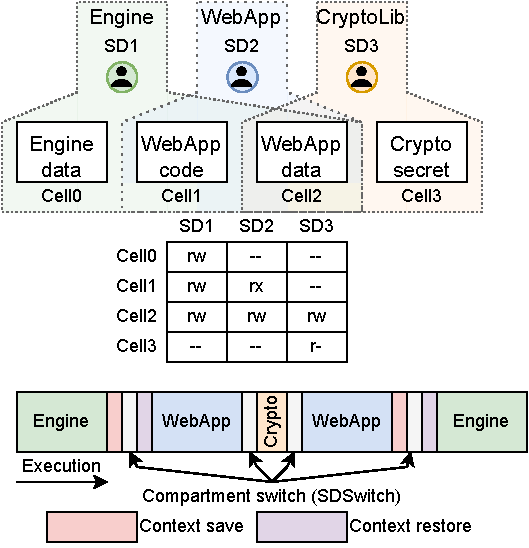
\includegraphics[width=0.65\linewidth]{media/seccells/browser_webapp.pdf}
  \caption{Browser compartmentalization with three compartments.}
  \label{fig:seccells:browser_eg}
  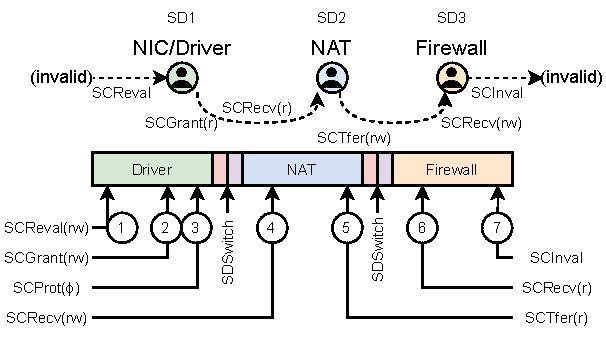
\includegraphics[width=\linewidth]{media/seccells/dataflow_app.pdf}
  \caption[Permission transfers for a packet between \seccells compartments.]
          {Permission transfers for a packet between \seccells compartments. 
            The figure shows the compartment executing the relevant \seccells 
            instructions on one core.}
  \label{fig:seccells:dataflow_app}
  %\Description[<short description>]{<long description>}
\end{figure}

\paragraph{Use case: Browser}
The first program, a browser (\autoref{fig:seccells:browser_eg}), consists of
a just-in-time (JIT) compilation engine (Engine), 
a sandboxed web application (WebApp) compiled and executed by the Engine, and 
a cryptographic library (CryptoLib) storing a secret key for encryption.
The compartmentalization policy aims to isolate the Engine's data
and CryptoLib's secret from the possibly malicious WebApp.
Borrowing the threat model for browsers, we assume that the 
WebApp can exploit bugs in the Engine's compiler to 
generate and execute arbitrary code as the WebApp compartment,
ultimately aiming to leak the browser's data or the cryptographic secret.
The developer aims to prevent unauthorized inter-compartment data accesses
by enforcing the per-compartment permissions shown in the figure.
To maintain similar performance to the monolithic version, the developer
desires minimal overhead from operations added due to compartmentalization:
context switching and compartment switching.

\paragraph{Use case: Network Function Virtualization}
The second program is a virtual network function pipeline 
(\autoref{fig:seccells:dataflow_app}) consisting of three stages progressively
performing processing steps on a stream of packets.
In particular, this pipeline has three compartmentalized stages, 
implementing the network card driver (Driver) which
generates packets, 
a network address translation (NAT) stage which translates IP 
addresses in the header based on a translation table, and
a firewall stage that implements checks on the packet headers
based on a rule table.
In this example, we omit further stages for simplicity.
Middleboxes in datacenters and the internet~\cite{MartinsAROHBH14}
commonly contain virtual network functions sharing a buffer pool
in uncompartmentalized dataflow pipelines.
Translation and rule tables in the NAT and Firewall compartments
must be isolated in private regions, protecting them from potential bugs 
in the Driver compartment that processes input from untrusted traffic 
from external sources.
The programmer requires isolation of network stages for high reliability
of the middlebox and low cost for passing packets between stages for 
line-rate packet processing, enabled by zero-copy packet flow 
through permission transfer.


%-------------------------------
\subsection{Threat Model}
\label{sec:seccells:reqs:threat}
%-------------------------------

Our threat model assumes an attacker who wants to compromise a 
compartmentalized program with multiple communicating compartments.
We assume that the attacker has compromised one or more compartments, and
gained the ability to both generate arbitrary code and execute it,
but is restricted to the compromised compartments.
The attacker wishes to compromise confidentiality, integrity, or 
gain code execution in other compartments.
%
For example, the attacker might try to:
% \begin{inparaitem} for an inlined bullet point list instead
\begin{itemize}
  \item gain permissions and directly access (load/store) 
        another compartment's private memory,
  \item inject unsolicited code/data regions in another 
        compartment's memory,
  \item execute unintended code in another compartment,
  \item create new compartments, or
  \item achieve any combination of the above.
\end{itemize}

The policy used for compartmentalization is assumed to be sound, and the software
implementations of the modules comprising compartments are assumed to be
free of bugs that can be exploited via only their exposed communication
interfaces.
\seccells' trusted computing base (TCB) consists of the hardware implementation
and the supervisor.
Exploitable bugs in the policy or TCB can lead to a compromise irrespective of the
compartmentalization mechanism.
While speculative side-channel attacks are outside the scope of our threat model,
we discuss \seccells' speculative resiliency in \autoref{sec:seccells:discussion}.

%-------------------------------
\subsection{Security Objectives}
\label{sec:seccells:reqs:security}
%-------------------------------
A secure mechanism must enforce restrictions on a compartmentalized program,
as described below.

\paragraph{Obj. \req{1a}}
Mechanisms must implement \emph{access control},
validating every memory access against the policy.
For the browser in \autoref{fig:seccells:browser_eg}, the table
holds policy-defined permissions for each compartment and memory region.
Mechanisms must, for example, prevent all accesses by the compromised
WebApp from reading the Engine or CryptoLib's private regions as per the
policy.
Mechanisms must also prevent corruption of policy-defined permissions
stored in memory or registers.
Intel MPK-based protection~\cite{ParkLXMK19}, for example, loads
permissions from a user-controlled register when executing a
\Code{wrpkru} instruction, allowing a compartment to corrupt its 
own permissions.

\paragraph{Obj. \req{1b}}
Inter-compartment communication consisting of cross-compartment calls 
demand \emph{validity checks}.
Relevant validity checks include checking that 
\begin{inparaenum}[\itshape i\upshape)]
  \item the entry point is valid,
  \item the calling compartment is allowed to call the target compartment, 
  \item the return respects the call stack, and
  \item the passed arguments are valid.
\end{inparaenum}
Compartment switches from the WebApp to the Engine must use valid entry
points which are followed by argument-validating code. Failure to enforce this
constraint enables
control-flow attacks such as return-oriented programming (ROP).
Vanilla Intel MPK-based protection also lacks such entry-point checks
to accompany \Code{wrpkru} instructions.

\paragraph{Obj. \req{1c}}
\emph{Context isolation} accompanying a cross-compartment call is 
essential for protecting mutually distrusting compartments.
After a cross-compartment call, the callee compartment (for example, the Engine) 
must be able to fetch its context without trusting the registers which
are controlled by the caller (correspondingly, the WebApp), 
representing an attack vector.
The WebApp, for example, could try to switch to the Engine with a malicious stack pointer
register, attempting to corrupt the Engine by reading from the wrong stack.
CODOM~\cite{VilanovaBNEV14}, for example, assumes a migrating thread model
and is vulnerable to attacks through an invalid register state.

\paragraph{Obj. \req{1d}}
Mechanisms that allow untrusted compartments to modify or transfer their 
permissions must prevent privilege escalation %~\cite{ZeldovichBKM06} 
through \emph{TCB-imposed limitations} on these operations.
Specifically, compartments should only be allowed to surrender access 
permissions or transfer existing permissions to other compartments.
A stage in the network function pipeline, for example, should not be allowed
to grant write permissions for a packet to the next stage if it has
read-only permissions.
Transferring permissions between compartments must also be mutual, requiring
explicit actions from both compartments.
One-directional permission transfers studied by 
Lipton~\textit{et. al.}~\cite{LiptonS77} 
allow compartments to either steal other compartments'
permissions (violating confidentiality) or
inject illegal data or code into other compartments (violating integrity).
Linux, which allows processes to specify their own permissions
when \Code{mmap}ing shared regions, violates this objective without 
syscall mechanisms like SECCOMP.

\paragraph{Obj. \req{1e}} 
\emph{Temporary exclusive access} to otherwise 
shared data regions enables compartments to use data regions safely,
preventing exploitation of double-fetches.
With exclusive access to a packet, the Firewall stage of the network function
pipeline can safely validate and use addresses in the packet header in-place 
(without copying), with the assurance that another corrupt stage cannot
concurrently modify the packet.
XPC~\cite{DuHXZC19XPC} recognizes this objective, allowing exclusive access
to a single region tracked by the Relay Segment register.

\paragraph{Obj. \req{1f}} 
\emph{Auditability}, the ability to easily determine the 
global access permissions, facilitates auditing compliance to a 
compartmentalization policy by checking which compartments have access to
which memory region.
A browser might regularly audit its permissions to ensure that the WebApp
has not escalated its privileges.
An audit for a mechanism with a centralized permissions store, 
such as page tables, must only check this store simplifying audits.
In contrast, an audit for CHERI~\cite{WatsonWNMACDDGL15} requires an 
expensive, full-memory scan since the set of memory regions accessible to a
compartment is the transitive closure of capabilities held in its registers,
along with capabilities held in any memory region accessible through these 
registers.

%-------------------------------
\subsection{Performance Objectives}
\label{sec:seccells:reqs:performance}
%-------------------------------
Low-overhead checks and operations allow performance-critical
programs to be compartmentalized.

\paragraph{Obj. \req{2a}} 
\emph{Single-cycle access verification} in the common case
is essential for core throughput.
While most mechanisms meet this objective in the best (not common) case, 
page-table based isolation mechanisms suffer from the limited scalability
of Translation Lookaside Buffers (TLBs) used to cache permissions.
Programs with large datasets can incur high TLB miss rates, with 
correspondingly high verification latency in the common case due to 
page-table walks.
UNIX process-based protection particularly suffers from this limitation since
modern Address Space ID (ASID)-tagged TLBs will effectively contain duplicate
entries for a shared page with separate permission for each compartment,
effectively dividing an already capacity-limited structure among 
compartments~\cite{HsuHEP16}.
This objective implicitly requires the mechanism to support
a sufficiently large number of compartments and data regions.
A mechanism with small limits, like Intel MPK which is restricted to
16 colors for data regions, will incur overheads from software workarounds
required to virtualize the corresponding resource~\cite{ParkLXMK19}.

\paragraph{Obj. \req{2b}} 
Cross-compartment calls are essential and
frequent for communication between fine-grained compartments
necessitating \emph{fast compartment switches}.
Fine-grained library isolation~\cite{GhosnKPLB21} requires compartment 
switches accompanying every function call to an untrusted library.
A program isolating short-running functions, 
such as AES encryption using hardware AES-NI extensions, 
can incur a compartment switch every tens or hundreds of 
cycles~\cite{AbdAllahAES}.
Specialized hardware instructions accessible from userspace are
essential for cheap compartment switches in tens of cycles.
Even the fastest supervisor-mediated compartment switch still costs
hundreds of cycles~\cite{WatsonWNMACDDGL15}.

\paragraph{Obj. \req{2c}}
\emph{Fast, zero-copy permission transfer} enables programs to 
efficiently move data between compartments.
Data copying for passing large buffers during 
compartment calls can overwhelm high-performance programs, 
such as our example network function pipeline.
Such applications typically pass packets by reference between 
unisolated stages profiting from zero-copy.
Cheap permission transfers, within ten to hundred cycles, enable 
such applications to be compartmentalized with performance
comparable to the monolithic versions.
UNIX process-based permission transfers instead involve microsecond-scale
system calls, precluding their use for practical compartmentalization.

%-------------------------------
\subsection{Flexibility}
\label{sec:seccells:reqs:flexibility}
%-------------------------------

A mechanism demands flexibility to be suitable
to compartmentalization across a variety of application domains. 

\paragraph{Obj. \req{3a}}
For flexibility, a mechanism must support \emph{arbitrary sharing of data
regions},
requiring independent per-compartment per-region permissions.
A private region, for example, should be accessible by only a single
compartment.
Another shared region might allow read access to one compartment, 
write access to another, and execute permissions to a third.
Mechanisms that target hierarchical security, for example, limit
flexibility --- the trusted  compartment implicitly has permission
to access an untrusted compartment's data --- and exclude wide 
applicability.
In contrast, even if the WebApp in the browser trusts the Engine,
the Engine is denied execute permissions to the WebApp's code.
A mechanism must support, but not be exclusive to, specific trust
models such as nested compartments.

\paragraph{Obj. \req{3b}}
To scale performance overheads with security objectives, we
introduce a desirable property, \emph{security-proportionality}.
A security-proportional mechanism allows policies to trade-off 
overheads for security when unnecessary.
Despite not trusting the WebApp, transitions from the WebApp to
CryptoLib can elide context switching required for register 
isolation under a specific condition.
Verification approaches~\cite{KolosickNJWLGJS22Verizero,ChenRSL16} 
can be used to prove that a small function in CryptoLib does not leak the key
under the assumption that entry points are enforced,
and that the function's code overwrites registers used to store the key 
before returning to the WebApp.
By using the cheaper migrating thread model~\cite{FordL94},
a security-proportional mechanism can reduce overheads where acceptable.
Process-based isolation, for example, is not security-proportional
since every compartment switch incurs the same non-negotiable overheads 
(including context switching, page-table switching, or scheduling).

%-------------------------------
\subsection{Alternate Visions for Compartmentalization}
\label{sec:seccells:reqs:related}
%-------------------------------

% Text for the camera ready. Reinstate.
\seccells envisions a future where the mechanism supports 
widespread application
compartmentalization efforts, with consequently differing goals
and designs compared to related mechanisms.
% \seccells targets different goals compared to related mechanisms
% consequently resulting in drastically differing designs.
% 
First, some mechanisms only support \emph{custom-tailored use cases}
such as differentiating between single trusted-untrusted 
compartments~\cite{HedayatiGJCSSM19Hodor,KoningCBGA17,Kilpatrick03}, % ,MogosanuRD18
or a binary classification of data as (in)sensitive~\cite{FrassettoJLS18}.
CODOMs~\cite{VilanovaBNEV14} link code addresses to compartments,
restricting code sharing that is abundant in modern programming.
Specialization allows simpler hardware mechanisms, but do not support
a broad spectrum of applications.
Second, \seccells does not aim to compartmentalize existing software with
zero-modifications.
While automated isolation techniques provide a crucial first step towards
compartmentalized programs~\cite{RoesslerAPMPKPB21,KirthDCLDGNVF22,
VasilakisKRDDS17}, security-critical software requires refactoring to fully
realize the benefits of proper compartmentalization.
Finally, related works target \emph{compatibility with legacy hardware}
or existing or upcoming software/hardware mechanisms and abstractions for 
isolation.
Numerous mechanisms try to compartmentalize using process-based isolation
implemented by the OS~\cite{LittonVE0BD16,DuHXZC19XPC,KleinEHACDEEKNSTW09}, 
retrofitting compartmentalization onto an abstraction originally designed for
multiprogramming on unicore processors.
Others leverage Intel MPK~\cite{HedayatiGJCSSM19Hodor,ERIMOberwagner19,KoningCBGA17}
or similar protection-key based mechanisms~\cite{SchrammelWSS0MG20Donky},
synergizing with traditional page table-based virtual memory.
Targeting immediate adoption, Hodor~\cite{HedayatiGJCSSM19Hodor} and 
LOTRx86~\cite{LeeSK18} (ab)used existing processor features intended for 
other purposes to isolate compartments.
HAKC~\cite{mckee2022preventing} leverages state-of-the-art ARM extensions, 
PAC and MTE, to compartmentalize the Linux kernel, but requires a two-level 
clustering of closely-connected compartments to overcome MTE's 
compartment scaling limitations and still incurs a significant performance hit.
With the sole exception of Mondrian~\cite{WitchelCA02MMP}, proposals
assume current page-based virtual memory.
Meanwhile, trends in applications and memory architectures have led to a 
resurgence in range-based translations and protections among academic 
proposals~\cite{BasuGCHS13,YanLNB19,PhamVJB12,0003BOBFP21midgard,KarakostasGACHM15}
and commercial processors including AMD's Zen lineup~\cite{preservingvma}.
\autoref{tab:seccells:req_comparison} summarizes the objectives satisfied by related 
mechanisms (justification in Appendix~\ref{app:seccells:justification_table1}).
We discuss related mechanisms further in \autoref{sec:seccells:related}.
 
% Camera ready TODO: Should I make figure and table styles consistent?
% If yes, follow the procedure described here
% https://tex.stackexchange.com/questions/166814/table-caption-in-uppercase-i-dont-know-why
\begin{table}
  \centering
  \caption[Qualitative comparison of compartmentalization mechanisms]
          {Comparison of compartmentalization mechanisms based on 
          compliance with the objectives described in \autoref{sec:seccells:reqs}.
          Limited compliance is marked with ``$\sim$''.
          }
% \begin{tabular}{l | c c c c c c | c c c | c c |}
  \begin{tabular}{l | c@{\hspace{1em}} c@{\hspace{1em}} c@{\hspace{1em}} c@{\hspace{1em}} c@{\hspace{1em}} c@{\hspace{1em}} | c@{\hspace{1em}} c@{\hspace{1em}} c@{\hspace{1em}} | c@{\hspace{1em}} c@{\hspace{1em}} |}
    \toprule
              & \multicolumn{6}{c|}{\req{1}}                  & \multicolumn{3}{c|}{\req{2}} & \multicolumn{2}{c|}{\req{3}} \\
              & a     & b     & c     & d     & e     & f     & a     & b     & c     & a     & b             \\ \midrule
  UNIX        & \yes  & \yes  & \yes  & N/A   &       & \yes  &       &       &       & \yes  &               \\
  Mondrian    & \yes  & \yes  & \yes  & N/A   &       & \yes  & \yes  &       &       & \yes  &               \\
  lwC         & \yes  & \yes  & \yes  & N/A   &       & \yes  &       &       &       & \yes  &               \\
  CODOM       & \yes  & \yes  &       & N/A   &       & \yes  &       & \yes  &       &       & \yes          \\
  XPC         & \yes  & \yes  & \yes  & \yes  & \yes  & \yes  &       & \yes  & $\sim$& \yes  &               \\
  MPK         &       &       &       &       &       & $\sim$&       & \yes  & \yes  & \yes  & \yes          \\
  ERIM        & $\sim$& $\sim$&       &       &       & $\sim$&       & \yes  & \yes  & \yes  & \yes          \\
  Donky       & $\sim$& \yes  &       & N/A   &       & \yes  &       & \yes  & \yes  & \yes  &               \\
  CHERI       & \yes  & \yes  & \yes  &       &       &       &       &       & \yes  & \yes  &               \\
  \seccells   & \yes  & \yes  & \yes  & \yes  & \yes  & \yes  & \yes  & \yes  & \yes  & \yes  & \yes          \\ \bottomrule
  \end{tabular}
  \label{tab:seccells:req_comparison}
\end{table}

\paragraph{Complementary requirements}
To satisfy application requirements,
programs compartmentalized with \seccells' mechanisms require
complementary properties from other parts of the system
including secure compartmentalization policies, 
a secure and performant supervisor interface, 
and formal verification of application-level properties
aided by programming conventions.
For example, supervisors might include a syscall for 
microsecond-scale compartment creation~\cite{LittonVE0BD16}.
Safe calling conventions can provide formal guarantees against
inadvertent information leakage from the stack~\cite{SkorstengaardDB20}.
These investigations are outside the scope of this thesis.

\paragraph{\seccells overview}
\seccells is a compartmentalization mechanism designed
to satisfy the above objectives across a wide array of 
programs, providing flexibility and performance without compromising on 
security.
\seccells stores permissions in a centralized permissions table accessible 
only by the supervisor and hardware.
A novel, range-based memory management unit (MMU) and 
lookaside buffer design (\autoref{sec:seccells:design:access_ctl})
allows single-cycle access control on the fast path satisfying 
objectives \req{1a}, \req{1f}, \req{2a}, and \req{3a}.
\seccells introduces fast, userspace instructions for common 
compartmentalization operations (see \autoref{tab:seccells:seccell_ops}): 
switching compartments, transferring permissions and validating
exclusive access for data regions (\autoref{sec:seccells:design:instructions}).
These instructions satisfy requirements \req{1b}, \req{1e},
\req{2b}, \req{2c}.
\seccells delegates context isolation, call-stack maintenance,
and argument validation to software.
\autoref{sec:seccells:design:softmech} outlines how software can
securely and efficiently implement context isolation and call-stack 
maintenance.
Software implementing these functions satisfy security (\req{1b}, \req{1c})
and flexibility (\req{3a}, \req{3b}) objectives.

%%%%%%%%%%%%%%%%%%%%%%%%%%%%%%%%
\section{\seccells}
\label{sec:seccells:design}
%%%%%%%%%%%%%%%%%%%%%%%%%%%%%%%%

\begin{figure}
  \centering
  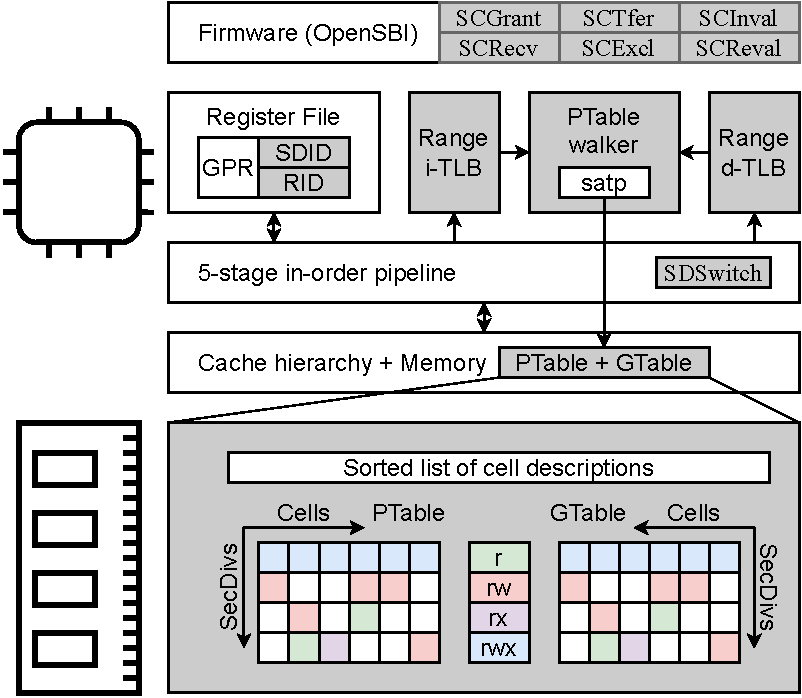
\includegraphics[width=0.85\linewidth]{media/seccells/seccell_arch.pdf}
  \caption[\seccells: Architecture.]
          {\seccells' architecture, highlighting modified hw/sw in gray.}
  \label{fig:seccells:seccell_arch}
  %\Description[<short description>]{<long description>}
\end{figure}

\seccells proposes hardware-software co-design to satisfy the
manifold objectives for efficient and secure compartmentalization.
The key insight that \emph{compartmentalization operations from untrusted userspace
are secure with TCB-maintained permission checks} allows \seccells to
implement compartment switch and permission transfer through
trusted hardware-checked userspace instructions which are
hundred to thousand times faster compared to traditional supervisor calls.
Pragmatically, \seccells retains software for operations such as 
context switching which, while common, would not benefit significantly 
from hardware support.
Software implementations of such operations achieve higher flexibility and
resilience to implementation errors at negligible or low additional performance
cost compared to a hardware implementation.
% Hardware compartment switching eliminates generic supervisor-dependent 
% overheads due to system call dispatch, scheduling and resource accounting, 
% as well as an extra context switch and pipeline serialization for entering
% the kernel.
For example, both hardware and software context switching can saturate
the L1 data cache bandwidth, achieving similar performance.
The second insight is that VMA-based permission tracking eliminates 
permission duplication inherent in page-table entries for pages 
within a VMA.
\seccells leverages this insight, eliminating overheads for 
permission storage (compared to equivalent page tables) and 
allowing hundred-times smaller core-side lookaside buffers. 

\seccells protects compartments, application-defined mutually untrusting
parts of a program, by controlling their access to memory regions.
Each compartment is allocated a Security Division (\secdiv)
with individual permissions to each VMA-granularity data region (\cell{}).
The Browser (\autoref{fig:seccells:browser_eg}), for example, has 
three compartments (Engine, WebApp and CryptoLib) allocated 
\secdivx{1}-\secdivx{3}, and four \cell{}s.
\seccells augments each core with a read-only register (\sid) tracking 
the currently executing compartment.
Along with a table for storing permissions (\ptable) and a modified
MMU for enforcing the permissions, \seccells implements single-cycle
access control.
The WebApp \secdiv has executable permissions
to one code \cell and read-write permission to one data \cell.
Userspace instructions (see \autoref{tab:seccells:seccell_ops}) enable 
secure compartment switching and permission surrender/transfer.
% For implementation reasons regarding how risc-v wants to use ecalls to enter
% the kernel, we must make urid writable by the kernel in our prototype.
% In a pure seccells world, where sdswitches are used for syscalls, we
% might no longer need writable urid (caveat switching programs).
%
% Mat: we could argue that privileged world can always write/override but this
% may be too implementation specific
Another per-core read-only register (\rid) tracks the caller after a 
compartment switch, allowing the callee to securely identify 
its caller.
% \andres{Not sure if this argument is enough, we can use a memory
% segment for that and rely on a compartmentalization policy (memory segment not
% writable by the callee). Is the performance argument sufficient?}
% Atri: Not sure how that would work
During permissions transfer, a granted permissions table (\gtable) tracks
outstanding permissions.
Further, the design implements context isolation and secure call stacks
in software leveraging the above hardware primitives.
\autoref{fig:seccells:seccell_arch} summarizes \seccells's architecture.
The detailed layout of cell descriptors, the \ptable, and the \gtable 
are shown in Appendix~\ref{app:seccells:ptable}.


%-------------------------------
\subsection{Access control}
\label{sec:seccells:design:access_ctl}
%-------------------------------
The Permissions Table (\ptable) stores 
per-cell, per-\secdiv permissions for the compartmentalized 
program.
For each \cell, the permissions for each \secdiv are independent
and define the degree of sharing for that \cell.
Compartment-private data stores allow only one \secdiv non-null 
permissions in this table.
Shared \cell{}s can be readable, writable, or executable by more than one
\secdiv.
For a JIT compiler, the \cell holding generated data will be writable
by the compiler \secdiv, while being executable by the sandboxed code's
\secdiv.
The \ptable is stored in privileged supervisor memory, restricting
accesses (including stores) from userspace.
\autoref{fig:seccells:browser_eg} shows the permissions for the three browser 
compartments, assigned to separate \secdiv{}s, to the four 
data regions, similarly assigned to \cell{}s.
\seccells' current \ptable design supports a large number of 
\secdiv{}s and \cell{}s ($2^{29}$ and $2^{32}$ respectively), 
vastly exceeding application requirements.
A finely-compartmentalized modern browser, for example, will only require
a few hundred compartments, isolating each loaded shared 
library (around 100 on the author's Firefox installation)
and per-tab rendering compartments~\cite{barth2008security}.

\seccells replaces the core's MMU with a \ptable walker and 
range-based lookaside buffers for permissions and translations.
The MMU checks access permissions based on the accessed address and
the executing \secdiv identified by the core's \sid register.
The lookaside buffers track a small number of frequently accessed
\cell{}s, along with \sid-tagged permissions.
In the common case, access control verifies permissions from
entries in this buffer.
When accesses miss in this buffer, the \ptable walker reads the
required permission from the \ptable.
The walker first performs a (fast) binary search in a sorted list of permissions
to find the correct cell containing the accessed address, then
reads the correct permission from the \ptable for that cell.
The location of the permission in the \ptable is found through very 
simple arithmetic.

\seccells' \ptable layout and MMU design has three
key advantages: fast \ptable walks, scalability to large data 
working sets, and low silicon cost.
The \ptable layout aids fast permission lookups by
sorting the \cell descriptors, allowing a binary search
for the \cell descriptor containing an address, 
and the contiguous layout of the permissions for a particular
\secdiv, which improves spatial locality for \ptable walks.
Range-based lookaside buffers also enable scalability for
programs with large datasets, since permissions should be 
verified against TLB entries in the common case.
With growing dataset sizes, traditional processors require larger 
TLBs in order to track additional page translations and permissions.
Importantly, all permissions for pages within a VMA are
the same, leading to duplication in TLB entries' permissions.
However, the growth of program datasets has exceeded the
TLB reach of modern processors, leading to attempts at 
range-based translations (explicitly managed by the 
supervisor~\cite{YanLNB19}, or implicitly through 
coalescing~\cite{PhamVJB12}).
In contrast, as dataset sizes grow, the \cell count remains 
constant and the size of \cell{}s increases.
Previous work in range-based translation caching~\cite{YanLNB19,0003BOBFP21midgard} 
have also demonstrated that 
processors require hundred-times smaller range-based lookaside buffers 
than in traditional systems, drastically reducing silicon cost.
Research proposals~\cite{0003BOBFP21midgard, ZhangSRL10} 
have also tackled
external fragmentation from range-based translations 
by introducing a system-wide page table after the
last-level cache.

%-------------------------------
\subsection{Userspace Instructions}
\label{sec:seccells:design:instructions}
%-------------------------------

\begin{table}[]
  \centering
  \caption{Overview of \seccells' userspace instructions.}
  \begin{tabular}{l | l}
    \toprule
    Instruction & Purpose                                           \\
    \midrule
    \sdswitch   & Switch to another \secdiv                         \\
    \scprot     & Change current \secdiv{}'s permission to \cell    \\
    \scinval    & Mark a \cell invalid                              \\
    \screval    & Revalidate an invalid \cell                       \\
    \scgrant    & Grant \cell permissions to another \secdiv        \\
    \screcv     & Accept granted \cell permissions                  \\
    \sctfer     & Grant and drop \cell permissions                  \\
    \scexcl     & Check for exclusive access to a \cell             \\
    \bottomrule
  \end{tabular}
  \label{tab:seccells:seccell_ops}
\end{table}

\begin{figure*}[!t]
  \vspace{-1\baselineskip}
  \rule{\textwidth}{1pt}
  \centering
  \textbf{\seccells Program State\\}
  \vspace{-0.5\baselineskip}
  \rule{\textwidth}{1pt}
  \vspace{-2\baselineskip}
  \begin{multicols}{2}
    \begin{algorithmic}[1]
      \State $S$ = Set of $M$ \secdiv{}s incl. supervisor $SD_{sup}$
      \State $C$ = Set of $N$ cells, each valid or invalid
      \State Per-core register $SID$
      \State Per-core register $RID$
      \State \ptable $PT: S \times C \mapsto \mathscr{P}(\set{r, w, x})$
      \State \gtable $GT: S \times C \mapsto S \times \mathscr{P}(\set{r, w, x})$
    \end{algorithmic}
  \end{multicols}
  \vspace{-1.4\baselineskip}
  \rule{\textwidth}{1pt}

\vspace{-0.7\baselineskip}
\begin{multicols}{2}
\removelatexerror

    % General notation:
    % c_i         for a cell
    % SD_j        for a secdiv
    % p_{i,j}     for PT(SDj,ci)
    % gp_{tgt}    for GT perms

    % SDSwitch algorithm
    \begin{algorithm}[H]
      \caption{SDSwitch($addr$, $SD_{tgt}$) \\
        Switch to $SD_{tgt}$ at instruction pointer $addr$   }
        \begin{algorithmic}[1]

          \State $c_i \gets cell(addr)$
          \State \textbf{assert} $valid(c_i)$

          \State \textbf{assert} instruction at $addr$ is $SDEntry$
          \State \textbf{assert} $x \in PT(SD_{tgt}, c_i)$
          \State instruction pointer $\gets addr$
          \State $RID \gets SID$
          \State $SID \gets SD_{tgt}$
        \end{algorithmic}
        \label{alg:sdswitch}
    \end{algorithm}
    \vspace{-0.5\baselineskip}

    % SCProtect algorithm
    \begin{algorithm}[H]
      \caption{SCProt($addr$, $perm$) \\
      Restrict rights to $addr$ to $perm$              }
      \begin{algorithmic}[1]

        \State $c_i \gets cell(addr)$
        \State \textbf{assert} $valid(c_i)$

        \State $p_{i,cur} \gets PT(SD_{cur}, c_i) $
        \State \textbf{assert} $perm \subseteq p_{i,cur}$

        \State $PT(SD_{cur}, c_i) \gets perm$
      \end{algorithmic}
      \label{alg:scprotect}
    \end{algorithm}
    \vspace{-0.5\baselineskip}

    % SCGrant algorithm
    \begin{algorithm}[H]
      \caption{SCGrant($addr$, $SD_{tgt}$, $perm$) \\
      Grant $SD_{tgt}$ $perm$ rights to $addr$             }
      \begin{algorithmic}[1]

        \State $c_i \gets cell(addr)$
        \State \textbf{assert} $valid(c_i) \land perm \ne \phi$

        \State $p_{i,cur} \gets PT(SD_{cur}, c_i)$
        \State \textbf{assert} $perm \subseteq p_{i,cur}$

        \State $GT(SD_{cur}, c_i) \gets (SD_{tgt}, p_{tgt})$
      \end{algorithmic}
      \label{alg:scgrant}
    \end{algorithm}
    \vspace{-0.5\baselineskip}

    % SCRecv algorithm
    \begin{algorithm}[H]
      \caption{SCRecv($addr$, $SD_{src}$, $perm$) \\
      Accept $perm$ rights to $addr$ from $SD_{src}$      }
      \begin{algorithmic}[1]

        \State $c_i \gets cell(addr)$
        \State \textbf{assert} $valid(c_i) \land perm \ne \phi$

        \State $(SD_{tgt}, gp_{tgt}) \gets GT(SD_{src}, c_i)$
        \State $p_{i,cur} \gets PT(SD_{cur}, c_i)$
        \State \textbf{assert} $SD_{cur} = SD_{tgt} \land perm \subseteq gp_{tgt}$

        \If{$perm = gp_{tgt}$}
          \State $GT(SD_{src}, c_i) \gets (SD_{inv}, \phi)$
        \Else
          \State $GT(SD_{src}, c_i) \gets (SD_{tgt}, gp_{tgt} - perm)$
        \EndIf
        \State $PT(SD_{cur}, c_i) \gets perm \cup p_{i, cur} $

      \end{algorithmic}
      \label{alg:screcv}
    \end{algorithm}
    \vspace{-\baselineskip}

    % SCTfer algorithm
    \begin{algorithm}[H]
      \caption{SCTfer ($addr$, $SD_{tgt}$, $perm$) \\
      Transfer all $perm$ rights for $addr$ to $SD_{tgt}$    }
      \begin{algorithmic}[1]
        \State SCGrant($addr$, $SD_{tgt}$, $perm$)
        \State SCProtect ($addr$, $\phi$)
      \end{algorithmic}
      \label{alg:tfer}
    \end{algorithm}
    \vspace{-1.5\baselineskip}

    % SCReval algorithm
    \begin{algorithm}[H]
      \caption{SCReval($addr$, $perm$)  \\
      Re-validate address $addr$ with $perm$ rights}
      \begin{algorithmic}[1]

        \State $c_i \gets cell(addr)$
        \State \textbf{assert} $invalid(c_i) \land perm \ne \phi$

        \State Validate $c_i$
        \State $PT(SD_{cur}, c_i) \gets perm$

      \end{algorithmic}
      \label{alg:screval}
    \end{algorithm}
    \vspace{-1.5\baselineskip}

    % SCInval algorithm
    \begin{algorithm}[H]
      \caption{SCInval($addr$)  \\
      Invalidate $addr$ cell}
      \begin{algorithmic}[1]

        \State $c_i \gets cell(addr)$
        \State \textbf{assert} $valid(c_i)$

        \ForAll{$SD_j \in S - \set{SD_{sup}, SD_{cur}}$}
          \State $p_{i, j} \gets PT(SD_j, c_i)$
          \State $(SD_{tgt}, gp_{tgt}) \gets GT(SD_j, c_i)$
          \State \textbf{assert} $p_{i,j} = \phi \land gp_{tgt} = \phi \land SD_{tgt} = SD_{inv}$
        \EndFor

        \State $PT(SD_{src}, c_i) \gets \phi$
        \State $GT(SD_{cur}, c_i) \gets (SD_{inv}, \phi)$

        \State Invalidate $c_i$
      \end{algorithmic}
      \label{alg:scinval}
    \end{algorithm}
    \vspace{-1.5\baselineskip}

    % SCExcl algorithm
    \begin{algorithm}[H]
      \caption{SCExcl($addr$, $perm$) \\
      Verify exclusive $perm$ rights to $addr$       }
      \begin{algorithmic}[1]

        \State $c_i \gets cell(addr)$
        \State \textbf{assert} $valid(c_i) \land perm \ne \phi$

        \State $p_{i,cur} \gets PT(SD_{cur}, c_i) $
        \State \textbf{assert} $perm \subseteq p_{i,cur}$

        \State $ (SD_{tgt}, gp_{tgt}) \gets GT(SD_{cur}, c_i)$
        \If{$ perm \cap gp_{tgt} \neq \phi$}
          \State \textbf{return} $False$
        \EndIf

        \State $excl \gets True$
        \ForAll{$SD_j \in S - \set{SD_{sup}, SD_{cur}}$}
          \State $p_{i,j} \gets PT(SD_j, c_i)$
          \State $(SD_{tgt}, gp_{tgt}) \gets GT(SD_j, c_i)$
          \If{$ perm \cap p_{i,j} \neq \phi \lor perm \cap gp_{tgt} \neq \phi$}
            \State $excl \gets False$
          \EndIf
        \EndFor
        \State \textbf{return} $excl$
      \end{algorithmic}
      \label{alg:sccount}
    \end{algorithm}
    \vspace{-\baselineskip}
  \end{multicols}

  \caption{\seccells' state and userspace instructions.}
  \label{fig:seccell_ops_formal}
\end{figure*}


\seccells introduces 8 new serializing userspace instructions for
accelerating common compartmentalization operations 
(\autoref{tab:seccells:seccell_ops}).
These instructions, formally defined in \autoref{fig:seccells:seccell_ops_formal}, 
implement speculation-free compartment switching with 
checked entry points, permission surrender and transfer for zero-copy dataflow.

The \sdswitch instruction targets secure, 
low-overhead compartment switching within userspace.
\sdswitch resembles function call instructions, with 
direct and indirect variants, additionally switching the
core's \sid register and saving the caller's \sid to \rid.
Since the \sid register is not writable from userspace, 
inter-compartment calls must use \sdswitch.
The cost of executing an \sdswitch is essentially the
cost of pipeline serialization, plus the negligible cost
of updating core registers, making it extremely cheap.
For an in-order 5-stage pipeline, an \sdswitch instruction
completes in around 8 cycles.
For an out-of-order processor, pipeline serialization is an 
essential cost incurred by all related mechanisms
to prevent Spectre-like~\cite{KocherHFGGHHLM019}
speculative execution attacks, typically requiring 50-100 cycles.
For example, serialization dominates ERIM's MPK-based 
99-cycle switch latency.
Compared to supervisor-controlled compartment switching, 
\sdswitch eliminates the cost of serialization on supervisor entry, 
context switches on entry and exit, syscall dispatch, scheduling, 
and accounting costs.

\seccells requires \sdswitch instructions for both
forward and backward edges on cross-compartment calls.
We show how software can implement cheap, secure call
stacks in \autoref{sec:seccells:design:softmech}.
Programs are also allowed more flexibility, and can implement
both remote procedure call (RPC)-like call-and-return (as in
\autoref{fig:seccells:browser_eg})
and circular function call graphs with one-way switches 
(as in \autoref{fig:seccells:dataflow_app}).

\sdswitch instructions impose an additional
restriction over function calls in order to enforce call gates --- 
the instruction at the target address must be
an executable \sdentry instruction for the target \secdiv.
This requirement limits the valid entry points for a compartment
to the executable \sdentry instructions in its code, 
and is conceptually similar to Intel's CET~\cite{intelCET}.
A compartment can mark valid entry points with \sdentry 
instructions, and implement call gates directly afterwards.
Note that while our attacker can inject arbitrary code into a
compromised \secdiv, it cannot write code into
any other \secdiv, protecting uncompromised \secdiv{}s from 
attack via code injection containing unintended entry points.
The only remaining way for an attacker to propagate between 
compartments is by using valid interfaces.
Proper input validation, which is always crucial for 
compartmentalized programs, protects against this attack vector.
In contrast, Intel MPK-based methods allow an attacker to
inject and execute a \Code{wrpkru} instruction into a compromised 
compartment to elevate its privileges to access all memory.
Further, the core executing \sdswitch updates the \rid
register with the caller's \sid,
allowing the callee to identify and validate the caller.

The \scprot instruction allows a \secdiv to update
its permissions to a \cell, with the restriction that the
new permissions are a strict subset of existing permissions.
Essentially, \scprot allows a \secdiv to surrender permissions
when no longer needed.
This instruction supports a common paradigm in secure software
where a program drops permissions as soon as possible.

An \scgrant-\screcv instruction pair, executed by
separate compartments, allows permissions for a \cell to be 
transmitted between them.
When the granting \secdiv executes \scgrant, the targeted
\sid and permissions are stored in the \gtable.
A \secdiv is only allowed to grant permissions it already has.
Only the targeted \secdiv can later accept these permissions
by executing an \screcv, specifying the \secdiv it expects to
receive permissions from.
Mutual involvement in permission transfers prevents \secdiv{}s
from ``stealing'' from or ``injecting'' into other \secdiv{}s'
permissions, ensuring confidentiality and integrity respectively.
Note how this prevents malicious code injection in particular,
including where an attacker might try to inject new entry 
points (\sdentry instructions).
Recognizing a common software pattern where a \secdiv hands over 
its permissions to the next stage and drops its own permissions, 
\seccells introduces the \sctfer instruction.
Unlike \scgrant, a \secdiv executing \sctfer also drops its
own permissions to the \cell involved.
The semantics of \sctfer are identical to consecutive \scgrant and 
\scprot instructions, but \sctfer deduplicates permission checks.
All data transfer instructions (\scprot, \scgrant, \sctfer, \screcv)
also flush the relevant entry from the MMU's lookaside buffer.
The network function is dependent on these instructions to
progressively transfer permissions to a packet between stages,
as illustrated in \autoref{fig:seccells:dataflow_app}.
However, a \secdiv can only have a single outstanding grant for
a particular cell. 
If a \secdiv grants a second set of permissions to a \cell before
the first set of permissions to the same \cell is accepted,
the first grant will be overwritten in the \gtable.

The \scinval-\screval instruction pair allows dataflow pipelines
to optimize the end and beginning of dataflow pipelines
such as the aforementioned network function pipeline.
The pipeline stages progressively drop permissions to the \cell
holding a packet, and finally wish to drop all permissions after the 
final stage.
However, dataflow pipelines reuse the \cell{}s to hold packets,
implying that the Driver \secdiv must find a way to regain
write permission to the \cell to write a new packet's contents
to it.
While this use case seems to require an illegal privilege escalation 
\textit{prima facie}, the fact that the end of the pipeline ``discarded''
the \cell holding the packet implies that its contents are trash,
and allowing another \secdiv escalated permissions to the \cell
is secure.
To support such usage, \seccells introduces the concept of validity
for a \cell.
The \scinval allows a compartment to explicitly state that a
\cell holds trash and is available for reuse.
On executing this instruction, this \cell becomes unavailable for
memory accesses and cannot be used by any instruction apart from
\screval.
The \screval allows any compartment to re-validate and use an
invalid \cell with arbitrary permissions.
\seccells imposes a key restriction in order to secure \cell reuses.
A \secdiv can only invalidate a \cell when it has exclusive access
to it, requiring all other sharers to explicitly drop their
permissions to this \cell.
This restriction ensures that a malicious \secdiv cannot indirectly elevate its 
privilege to a shared \cell by using an \scinval-\screval sequence.

Exclusive access to a data region is critical to security and
performance, and \seccells introduces the \scexcl instruction for this 
purpose.
Apart from enabling invalidation of a \cell, exclusive access is also
important for safety in concurrent programming.
Concurrent access to data regions enables double fetch vulnerabilities
(such as time-of-check-to-time-of-use or \tocttou).
The \scexcl instruction allows a \secdiv to check whether it has
exclusive access to a \cell.
With exclusive access, a \secdiv can skip making private copies
of data for double fetches, improving performance.
Conversely, when the policy dictates that a \secdiv should have
exclusive access to a \cell, that \secdiv can verify compliance with
the policy using \scexcl.

%-------------------------------
\subsection{Software Mechanisms}
\label{sec:seccells:design:softmech}
%-------------------------------

\seccells delegates certain operations to software: 
argument validation for call gates, 
maintaining call stacks, and context switching for register context isolation.
Of these, argument validation is arbitrarily variable based on the
compartmentalization policy and best left for software checks in 
hardware-enforced call gates.
\secdiv{}s can determine their caller by reading the \rid 
register, and find arguments in register or memory, and implement
software checks as necessary.
Software maintained call stacks for inter-compartment calls 
allow flexibility of calling models,
simplifies hardware and remains secure.
The software can securely restore with the same performance as hardware,
making a hardware implementation unnecessary.
In-software operations also improve \seccells' security-proportionality
as these operations can be skipped for lower overheads when safe to do so.

\begin{figure}
  \centering
  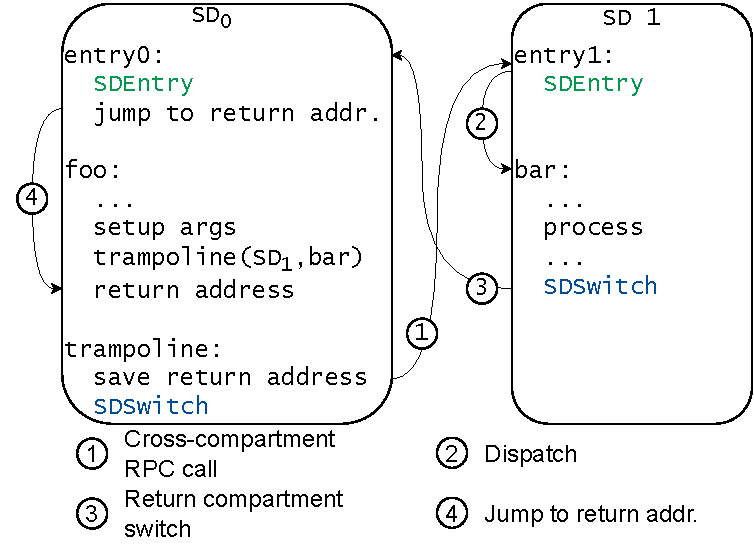
\includegraphics[width=0.7\linewidth]{media/seccells/sc_rpc.pdf}
  \caption{Cross-compartment procedure call in \seccells.}
  \label{fig:seccells:sc_rpc}
  %\Description[<short description>]{<long description>}
\end{figure}

Both forward and return edges on RPC-like cross-compartment 
calls use \sdswitch instructions, as illustrated in \autoref{fig:seccells:sc_rpc} 
where function \Code{foo} makes a cross-compartment call to \Code{bar}.
Arguments are passed in registers.
In this example, the caller uses a trampoline to hide its return address
before switching to \secdivx{1} (Step 1) and uses this address on the 
return path (Step 4).
\secdivx{0} is able to hide its calling address from \secdivx{1}, just
leaking the address of the generic trampoline.
Further, following the return switch to its entry point, \secdivx{0}
can read \rid to verify that the return is indeed from the called 
\secdiv, not any other.
On the other side, the callee (\secdivx{1}) can store its caller and
switch back to the caller's entry point on the backward edge.
If \secdivx{1} contains nested calls to other compartments, it
merely needs to remember its caller somewhere in its memory.
The dispatch (Step 2) secures the forward edge to \Code{bar} with call
gates.
While this example is secure, the flexibility of software allows other
calling patterns.

Context isolation requires the caller to save non-argument/return
registers to a state store before a \sdswitch and restore the same state
on the return edge.
The second step (context restore) is challenging since it
requires the \secdiv to find its state store without trusting any
register state, since the register state prior to the \sdswitch
persists.
We propose an array of per-\secdiv private \cell{}s as 
state stores, indexed by \sid.
The base of this array is easily constructed with
instruction pointer-relative instructions following an entry point.
Simple arithmetic involving the readable \sid register allows
a \secdiv to locate its state store, and consequently restore
the register state.
The latency of in-software context saving to memory is limited by 
the core's bandwidth to the L1 cache, the same as for any potential
hardware implementation.
Therefore, delegating this operation to software has no performance
impact.
Context switching also switches the stack pointer between 
per-compartment private stacks.

%-------------------------------
\subsection{Implementation}
\label{sec:seccells:impl}
%-------------------------------

Our implementation of \seccells augments and modifies the 
RocketChip~\cite{RocketChip} core and firmware.
An overview of the implementation is shown in 
\autoref{fig:seccells:seccell_arch}, with additions to the existing
processor highlighted in grey.
RISC-V provides the ideal, open platform for implementing fully-functional
prototypes of experimental architectures. 
\seccells permits a range of implementations for single and multi-core
processors containing in-order and/or out-of-order cores depending on the 
application's requirements: from firmware implementations on 
low-power embedded processors through hardware or 
microcode implementations on mobile, desktop, and server processors.
We discuss the trade-offs in detail in Appendix~\ref{app:seccells:impl_options}.
To match the RocketChip's simple, in-order pipeline, we implement 
access control and compartment switching in hardware within the pipeline 
and emulate the remaining instructions in firmware.

\seccells provides an alternate virtual memory mode, replacing 
SV-39 and SV-48.
We replace the core's MMU with a range-based TLB and a 
\ptable walker (replacing the traditional page-table walker).
We design the layout of the two-dimensional tables (\ptable and \gtable)
in memory to accelerate cell lookups and maximize 
spatial locality within the cache hierarchy when accessing permissions.
We add \sid and \rid to the core's Control-Status Registers (CSRs), 
and implement \sdswitch in the core pipeline.
The remaining instructions are implemented through hardware-assisted firmware 
by modifying OpenSBI~\cite{OpenSBI}.

The unified \ptable-\gtable in memory starts with a sorted
list of \cell descriptions, followed by the permissions held in the 
\ptable, and then the mappings for the \gtable.
% We don't have this layout any more
Appendix~\ref{app:seccells:ptable} shows the layout in detail.
Each \cell is described by the base and bound virtual addresses, 
the corresponding physical address base, and a single bit denoting
validity.
The sorted list of \cell{} descriptions allows the \ptable walker to
perform a binary search when looking for the cell which contains a particular
address, greatly accelerating lookups.
The row-major layout of the \ptable groups permissions for the same \secdiv
in contiguous cache lines, resulting in intra-cache line spatial locality for
permission lookups, and synergizing well with next-line prefetchers.
As a result, most MMU permission lookups are likely to be served by the L1 cache.
The unified \ptable-\gtable together occupies $\sim160kB$ to track permissions
to 1024 \cell{}s with 64 \secdiv{}s, equal to the memory used by leaf 
page-table entries to map $80$MB of data.

The range-based lookaside buffer holds a few \cell{} descriptions
and the corresponding permissions tagged by \sid.
The implementation of these structures is inspired by recent forays into 
range-based translation caches~\cite{0003BOBFP21midgard, YanLNB19, BasuGCHS13}, 
primarily aimed at tackling the limited reach of modern page-based translation 
lookaside buffers (TLBs).
Midgard~\cite{0003BOBFP21midgard} has shown that such lookaside buffers can 
sufficiently cover the working set of large applications with a 
few ($\sim$ 16) entries.

\seccells' userspace instructions are implemented through 
hardware-software co-design.
The \sdswitch instruction is implemented purely in hardware, and the
remaining permission-modifying instructions are emulated through firmware.
Additional hardware helpers, designed to aid operations trivially achieved
in hardware but costly in software, simplify and accelerate the emulation.
One notable operation is the lookup of the cell's index in the 
\ptable, which is common for all added instructions.
While a binary search in software is expensive, the MMU already holds this
information. 
We add an instruction, only accessible in RISC-V's machine mode and similar 
to the \Code{AT} instruction in ARMv8-A ISA~\cite{ARMAT}, to directly query the MMU.
We envision that higher performance processors with microcode sequencers
can implement these instructions in microcode, and
leave the investigation of the requirements of such an implementation
to future work.

%%%%%%%%%%%%%%%%%%%%%%%%%%%%%%%%
\section{Evaluation}
\label{sec:seccells:evaluation}
%%%%%%%%%%%%%%%%%%%%%%%%%%%%%%%%

In this section, we evaluate key metrics for \seccells' security and 
performance.
First, we show how \seccells provides security for the Browser described
in \autoref{sec:seccells:reqs}.
Second, we measure the latency of the \seccells' userspace instructions 
in microbenchmarks, particularly comparing compartment switching latency 
to related work.
We finally measure \seccells' performance for two representative workloads
highlighting the effect of range-based access control and
using userspace instructions for compartment switching and permissions
transfer.

\begin{table}
  \centering
  \caption{HW configuration of the \seccells prototype. }
  \begin{tabular}{l|c|c}
    \toprule
    Component             & \multicolumn{2}{c}{Configuration}                              \\
                          & Baseline                      & \seccells                      \\
    \midrule
    Core                  & \multicolumn{2}{c}{1 $\times$ Rocket, 6-stage, in-order}       \\
    L1 - D/I TLB          &  32-entry, fully-assoc.       & 16(D)/8(I)-entry, fully-assoc. \\
    L2 TLB                & 1024-entry, 4-way assoc.      & 32-entry, fully-assoc.         \\
    L1 D/I-cache          & \multicolumn{2}{c}{32KB, 8-way associative }                   \\
    L2 cache              & \multicolumn{2}{c}{16MB, 16-way associative}                   \\
    Main memory           & \multicolumn{2}{c}{DDR3, 800MHz, 1GB       }                   \\
    \bottomrule
  \end{tabular}
  \label{tab:seccells:testbench_cfg}
\end{table}



\begin{table}
  \centering
  \caption{FPGA resource utilization for SecureCells' MMU }
  \begin{tabular}{l | r  r  r | r  r  r}
    \toprule
                 & \multicolumn{3}{c|}{Traditional}  & \multicolumn{3}{c}{\seccells}  \\
                 & LUTs   & FFs   & SRAM             & LUTs & FFs   & SRAM            \\
    \midrule
    L1 ITLB      & 1915   & 1886  & 0                & 1529 &  869  & 0               \\
    L1 DTLB      & 2613   & 2048  & 0                & 1272 & 1903  & 0               \\
%   L2 TLB       & ----   & ----  & -                & ---- & ----  & -               \\
    L2 TLB + PTW & 5000   & 3428  & 18KiB            & 3826 & 4596  & 0               \\
%   Total(Core)  & ----   & ----  & -                & ---- & ----  & -               \\
    \midrule
    % \rowstyle{\bfseries}
    MMU Total    & 9528   & 7362  & 18KiB            & 6627 & 6200  & 0               \\
    \bottomrule
  \end{tabular}
  \label{tab:seccells:fpga_resource}
\end{table}

\paragraph{Testbench}
We ran the security evaluation on a QEMU implementation of \seccells,
which faithfully models its functional behavior, and the performance 
experiments on our hardware implementation of \seccells,
which uses cycle-accurate Register-Transfer Level (RTL) simulation to
accurately measure its timing behavior.
The core configuration, described in \autoref{tab:seccells:testbench_cfg}, 
resembles ARM's Cortex-A75. %~\cite{CortexA75}.
Our baseline is an identical core using a traditional page-based MMU
and TLBs instead of \seccells.
\autoref{tab:seccells:fpga_resource} shows the FPGA resource utilization for both the
baseline and \seccells MMUs.
\seccells' \ptable walker contains simpler logic than the baseline, 
as evidenced by the fewer LUTs required in the design.
Additionally, the much smaller range TLB eliminates the 18KiB block SRAM
required to store $1,024$ entries in the baseline L2 TLB.
We run our benchmarks on a seL4 kernel ported to use \seccells' 
memory protections. To evaluate realistic workloads on the seL4 kernel,
we faithfully ported core functionality of benchmarks, carefully limiting
system calls.

%-------------------------------
\subsection{Security Evaluation}
\label{sec:seccells:evaluation:sec}
%-------------------------------

To evaluate \seccells' security claims, we test that a properly 
compartmentalized \seccells program prevents common attack vectors
for monolithic software.
We also include an in-depth analysis of \seccells' instruction semantics
afterwards.

\paragraph{Access Control}
We evaluate \seccells' access control on a mock Browser,
modeling the example described in \autoref{sec:seccells:reqs}.
The Browser contains a simple compiler Engine that generates code for
sandboxed WebApp applications.
The WebApp can allocate arrays, and read/write elements in the array through
get/set instructions.
We emulate a buggy Engine that generates vulnerable WebApp code lacking bounds 
checks on array accesses, allowing the WebApp arbitrary reads and writes.
With the monolithic Browser, an attacker WebApp could leak/modify the
Engine's data as well as that of a second sandboxed WebApp.
When compartmentalized with \seccells with the permissions shown in 
\autoref{fig:seccells:browser_eg}, illegal accesses by the attacker WebApp outside its
data \cell instead raise load/store access faults.
\seccells' access control also prevents arbitrary code injection by the WebApp
by preventing the WebApp from writing to either its or the Engine's code regions.

\paragraph{Context Isolation and Call Gates}
When uncompartmentalized, the WebApp can modify the Engine's stack enabling
control- and data-flow attacks like ROP~\cite{Shacham07}.
Using \seccells for separation, inter-compartment calls between the 
Engine and the WebApp are protected through call gates 
implementing context isolation (\autoref{sec:seccells:design:softmech}) including
stack switching.
\seccells successfully prevents the WebApp from accessing the Engine's stack.

\subsubsection{Formal Description and Analysis of \seccells' 
Userspace Instructions}

We define the semantics of \seccells' unprivileged instructions
in \autoref{fig:seccells:seccell_ops_formal} and discuss their corresponding
security checks below.

\paragraph{\sdswitch}
This instruction checks that the jump target is valid, and holds
an \sdentry instruction executable by the target \secdiv.
With the precondition that the caller \secdiv does not have
writable permission to any \cell executable by the target \secdiv,
\sdswitch guarantees compartment entry at previously defined entry 
points (helping implement call gates). 

\paragraph{\scprot}
This instruction checks that the target \cell is accessible by the
\secdiv, and the new permissions are a subset of the existing permissions.
After this instruction, the \secdiv is assured to have no more permissions
than before.

\paragraph{\scgrant, \screcv and \sctfer}
\scgrant checks that the granting \secdiv has permissions to the
\cell, and that the granted permissions are a subset of its existing
permissions.
\screcv, in turn, checks that the \secdiv is receiving permissions for a
valid cell, that the permissions were previously granted by the
specific \secdiv that the receiving \secdiv expects, and that the received
permissions are a subset of the permissions granted.
\sctfer includes the checks of both \scgrant and \scprot.
The granting and receiving \secdiv{}s must cooperate in order to
transfer permissions, and together finish with the same or fewer
permissions than they began with.

A correct compartment is defined to not grant or receive any permissions 
or invalidate cells that it is not required to grant as per a correct
compartmentalization policy.
Considering a set of compromised attacker \secdiv{}s and their permissions 
to \cell{}s and assuming that uncompromised compartments are correct,
\seccells guarantees that the attackers can neither gain any new permissions 
through any sequence of permission transfer instructions 
nor elevate the permissions of any uncompromised compartment.
Using \scgrant and \screcv instructions, the compromised compartments can
transfer permissions between themselves but those grants cannot include 
permissions which none of the attackers had initially.
The only way for the attackers to gain permissions is from
an uncompromised \secdiv either granting permissions to a \cell or from 
invalidating a private \cell which one of the attackers can validate with \screval.
The only way for the attackers to inject permissions is to have an
uncompromised \secdiv receive them.
By definition, uncompromised compartments will do neither of the above.
Once again, we stress on the importance of a correct compartmentalization
policy.
No mechanism, including \seccells, can protect against an insecure policy
where compartments transfer permissions from/to untrusted compartments
without proper validation.

\paragraph{\scinval} 
This instruction allows a \secdiv to invalidate a \cell to which
it has exclusive access, and to which no outstanding permission grants
exist.
The first condition can be true for a private region, or for one
which other \secdiv{}s have willingly dropped permissions.
Consequently, no other \secdiv will unwittingly lose permissions to
the invalidated \cell as a consequence of \scinval.
The second condition provides the assurance that no compartment can
regain permissions to the cell without executing \screval.

\paragraph{\screval} 
This instruction checks that the address corresponds to an existing 
\cell{} and that it is currently invalid. 
Due to the initial invalidity of the \cell, no \secdiv{}s could have
access to the cell to be revalidated.

\paragraph{\scexcl}
This instruction does not modify any permissions, only allowing a
\secdiv{} to check if it has exclusive access to a \cell{} to which
it already has access to.


%-------------------------------
\subsection{Performance Microbenchmarks}
\label{sec:seccells:evaluation:perf}
%-------------------------------

% Comments on CHERI accounting:
% CHERI provided fine-grained overhead breakdown, which does not strictly
% conform to the
% categories in the aforementioned table. Therefore, we did need to figure
% out how to
% assign costs to categories. Therefore, the method is:
% Fixed costs       = kernel(receive trap) + kernel(exit kernel)
% context switching = caller + libcheri + kernel(clear non-arg registers)
% Switching cost    = Kernel SW operations
%       Switch	Ctx-switch	Other
%   42          42                       caller: Setup call, clear unused argument regs
%   34          34                       libcheri: Save callee-save regs, push call frame  
%   28  28                               kernel: Receive trap                               
%   79  79                               kernel: Validate CCall args.                       
%   41  41                               kernel: Push trusted stack, unseal CCall args.     
%   4   4                                kernel: Clear non-argument registers               
%   12  12                               kernel: Exit kernel                    
%   31  31                               kernel: Receive trap                               
%   7   7                                kernel: Validate return capability                 
%   4   4                                kernel: Clear non-return registers                  
%   41  41                               kernel: Pop trusted stack                          
%   7   7                                kernel: Exit kernel                                        
%   52          52                       libcheri: Pop call frame, restore regs.   
%   1           1                        caller: Back in caller                              
%--------------------------------------------------------------
%       254     129                      Total

\begin{table}
  \centering
  \caption{Compartment switching cost of \\various compartmentalization mechanisms.}
  \begin{threeparttable}
    \begin{tabular}{l | r | r | r | l | l}
      \toprule
                  & \multicolumn{3}{c|}{Round-trip Cycles}               & \multicolumn{2}{c}{CPU}   \\
                  & Switch         & \parbox[t]{1cm}{Context\\                                         
                                                     Saving}    & Total  & OoO\tnote{1} & Model      \\\midrule
      $lwC$       & \multicolumn{2}{c|}{$2 \times 6000$}        & 12000  & \checkmark   & SkyLake    \\
      seL4        & \multicolumn{2}{c|}{$2 \times 514 $}        & 1027   &              & RocketChip \\
      CHERI       & 254\tnote{2}   & 129\tnote{3}               & 425    &              & CHERI      \\
      ERIM        & $2 \times 99$  & Opt\tnote{5}               & 198    & \checkmark   & Xeon       \\
      XPC         & 82\tnote{4}    & Opt\tnote{5}               & 82     &              & RocketChip \\
      \seccells   & $2 \times 8$   & Opt\tnote{5}               & 16     &              & RocketChip \\
      \bottomrule
    \end{tabular}
    \begin{tablenotes}
      \item[1] Out-of-order CPUs incur higher pipeline serialization costs
      \item[2] In-kernel time
      \item[3] Userspace time (caller, libcheri)
      \item[4] XPC call + return + TLB miss
      \item[5] Optional, software-implemented context switch
    \end{tablenotes}
  \end{threeparttable}
  \label{tab:seccells:ipc}
\end{table}

\begin{table}[]
  \centering
  \caption{Cycles for emulating \seccells instructions.}
  \begin{tabular}{l | r | r | r | r}
    \toprule
    Instruction & \parbox[t]{0.7cm}{Trap\\ entry} 
                            & Dispatch  & Emulation & \parbox[t]{0.8cm}{Total \\Cycles} \\
    \midrule
    \scprot     & 79        &   32      &   33      & 144 \\
    \scinval    & 79        &   35      &   68      & 182 \\
    \screval    & 79        &   39      &   44      & 162 \\
    \screcv     & 79        &   54      &   69      & 202 \\
    \scgrant    & 79        &   52      &   63      & 194 \\
    \sctfer     & 79        &   61      &   62      & 202 \\
    \scexcl     & 79        &   57      &   67      & 203 \\
    \bottomrule
  \end{tabular}
  \label{tab:seccells:emulation}
\end{table}

First, we create microbenchmarks to measure the latency of each
userspace instruction introduced by \seccells, of which \sdswitch
is directly implemented in hardware, and the other instructions
are emulated in firmware.

In \autoref{tab:seccells:ipc}, we compare \seccells' compartment switching
cost with that of related mechanisms, particularly for a
round-trip cross-compartment call.
\seccells' userspace \sdswitch enables 8-cycle compartment switches,
with optional software context saving costs, which is more than $5\times$
faster than XPC's switch.
\sdswitch's latency consists of pipeline serialization (5 cycles), 
an instruction permission check (2 cycles) and a single cycle for the
targeted \sdentry instruction.
Of course, both XPC and \seccells would incur higher pipeline serialization
costs on an out-of-order core, putting \seccells on par with, or better than,
the MPK-based ERIM. 
Note that ERIM requires stringent code integrity and control-flow
integrity guarantees while \seccells does not impose any code requirements for
its compartmentalization guarantees.

All instructions other than \sdswitch and \sdentry are emulated by
the firmware, and therefore incur the costs of context saving, 
firmware entry and exit handlers, and dispatch to the correct
emulation function.
\autoref{tab:seccells:emulation} shows the latency of each instruction,
breaking down the cycles spent on each of the above overheads.
A microcode implementation of \seccells would allow the core to use 
internal registers for storage, eliminating the context switch, 
and directly lookup the microcode ROM to find the emulation 
microcode, eliminating dispatch.
Consequently, a microcode-based implementation would reduce 
\seccells' cost to that of the core emulation code only.

%-------------------------------
\subsection{Compartment Switching and Access Control}
%-------------------------------
To evaluate \seccells' practical performance, we create a simplified 
benchmark representative of a popular server workload, 
\Code{memcached}, accurately modelling the workload's memory access 
patterns across varying dataset sizes.
Our benchmark implements the core hashtable-based storage and the 
common query path loaded by an in-process load generator function
and omits system call-dependent features (networking, dynamic resizing),
and the global LRU list.
The benchmark isolates the data store from the vulnerable external interface
--- attackers might send malformed requests to trick the interface into directly
accessing the data store ---
by assigning them to separate \secdiv{}s.
The interface deserializes incoming requests, queries the data store
by switching compartments using \sdswitch, and serializes the
outgoing response.
For simplicity, this benchmark utilizes the migrating thread model.

\begin{figure}
  \centering
  \includegraphics[width=0.85\linewidth]{data/seccells/32ksim/mycached_full.pdf}
  \caption[\seccells performance comparison: \Code{memcached}]
          {Comparison of cycles-per-request,   
          cycles-per-instruction (CPI), and
          TLB miss rate
          while executing compartmentalized \Code{memcached} benchmark on 
          \seccells, compared to the uncompartmentalized version on RocketChip
          (lower is better).
          }
  \label{fig:seccells:mycached_cpi}
  %\Description[<short description>]{<long description>}
\end{figure}

Compartmentalizing the server allows us to measure the overheads
of frequent compartment switches, while varying the program's
dataset size allows us to compare \seccells' scalability.
We scale the dataset size by sweeping the number of fixed-size (64B)
entries stored in the data store, all of which are accessed randomly
by the load generator.
We compare the compartmentalized server running on \seccells'
implementation to an uncompartmentalized server running on
an unmodified RocketChip core by measuring the average count of
instructions retired and cycles used to process each request.
To compare against another emerging compartmentalization architecture,
we also conservatively model CHERI's performance on this benchmark,
adding the costs of supervisor-mediated compartment
switches with hardware support, as reported in the 
CHERI paper~\cite{WatsonWNMACDDGL15}.
We model each compartment switch as 191 instructions requiring 254 cycles,
excluding the costs of context switching and
ignoring other microarchitectural overheads.
In \autoref{fig:seccells:mycached_cpi}, we plot the average per-request 
cycle count and the cycles-per-instruction (CPI) for the server.

\seccells implements fast compartment switching, and 
the cost of switching to and from the data store compartment
for each request (16 cycles) is minuscule ($< 3\%$) compared to the
request processing time (minimum 532 cycles).
Consequently, \seccells' performance closely tracks that of 
the baseline even for small dataset sizes.
In contrast, CHERI's compartment switching overwhelms the
request processing time, only approaching the baseline's
performance for large dataset sizes.
While CHERI's performance for compartmentalization compares
favorably to that of traditional OS-based isolation 
techniques, it offers unacceptable overheads for finer, 
function-granularity compartmentalization (up to 95.5\%).

The CPI graph highlights the baseline system's limited TLB 
reach.
As the dataset exceeds the TLB reach of 4MB, the baseline starts
to encounter TLB misses on accesses to the data store.
Consequently, the baseline CPI starts to degrade compared to
\seccells, and only worsens as the dataset increases past the
CPU's last-level cache capacity.
In contrast, \seccells' range-based lookaside buffer comfortably
scales to large datasets, allowing the \Code{memcached} server to
serve requests 9.3\% faster for a 32MB dataset.
 
%-------------------------------
\subsection{Compartmentalized pipeline}
%-------------------------------

\begin{figure}
  \centering
  \includegraphics[width=0.85\linewidth]{data/seccells/network_1ktlb_sim/nfv_full.pdf}
  \caption[\seccells performance comparison: Network function]
          {Packet processing cycles-per-byte comparison.}
  \label{fig:seccells:nfv_cpb}
  %\Description[<short description>]{<long description>}
\end{figure}

To illustrate \seccells' zero-copy permission transfer performance,
we implement the virtual network function pipeline presented in
\autoref{fig:seccells:dataflow_app}.
The Driver stage generates a ``packet'' by writing a UDP/IP packet
of varying length into a packet buffer, whereas 
the Firewall and NAT read and modify the IP and UDP headers
respectively, but ignore the packet's payload.

Representing the ideal performance target,  we include the
``uncompartmentalized'' configuration that passes the packet by 
reference, incurring no overheads for data transfer.
The second configuration, ``compartmentalized-copy'', 
compartmentalizes pipeline stages and uses shared buffers to transfer
packets by copy.
The third, zero-copy ``\seccells ZC''  configuration isolates
stages, and uses userspace instructions to transfer 
access permissions to packets, each of which occupies a
different \cell{}.
Finally, the ``\seccells ZC-$\mu$code'' configuration models the 
possible performance of a microcode implementation of \seccells' 
dataflow instructions by mitigating trapping overheads
to the firmware and dispatch.
This model is conservative, ignoring possible optimizations from
parallelizing checks in microcode.

In \autoref{fig:seccells:nfv_cpb}, we plot the average number of cycles
required by the benchmark to process a byte of a packet
as the packet size grows.
Fixed costs, such as a function call, compartment switch or 
permission transfer, have diminishing impacts as the packet size grows.
The costs for generating and copying the packet, however, grows
linearly with packet size, and add a constant vertical offset in the
graph.
The ``compartmentalized-copy'' configuration incurs additional costs over the
uncompartmentalized baseline due to 
compartment switches (4.4\% for small packets) and packet copy (51.1\%).
The ``\seccells ZC'' configuration trades-off linearly-growing 
packet copying costs with fixed-cost permission transfers and
(in)validations.
While the $\sim250$-cycle average latency of \seccells' 
permission-modifying instructions causes a massive 199\% overhead
for the smallest packets, this fixed cost quickly gets amortized
for larger packets.
Indeed, this configuration overtakes the ``compartmentalized-copy'' configuration
for 600B packets and above, and approaches the performance
of the uncompartmentalized configuration (2.0\% overhead) for
16kB packets.
Finally, the ``\seccells ZC-$\mu$code'' configuration highlights \seccells'
performance potential, with (average) 69-cycle operations for 
transferring permissions which lowers the break-even threshold to
200B packets.

%%%%%%%%%%%%%%%%%%%%%%%%%%%%%%%%
\section{Related Work}
\label{sec:seccells:related}
%%%%%%%%%%%%%%%%%%%%%%%%%%%%%%%%

A variety of compartmentalization techniques exist, both in software and
leveraging hardware, targeting differing goals and with consequently
different designs.

Attacks often target specific, sensitive data for 
leakage or corruption (e.g., keys or flags).
Consequently, various proposals such as IMIX~\cite{FrassettoJLS18},
ERIM~\cite{ERIMOberwagner19}, and MemSentry~\cite{KoningCBGA17} introduced 
mechanisms to specifically protect 
such data from untrusted or unsafe code.
However, these mechanisms fail to apply to more generic scenarios,
with more than two compartments, per-compartment sensitive or private
data, and non-hierarchical trust models.
COde-centric memory DOMains~\cite{VilanovaBNEV14} proposed an architecture
where the instruction pointer identifies the running compartment, in a bid
to isolate untrusted libraries.
However, this proposal is unable to support the extensive code sharing 
in modern programs, including shared libraries like \Code{libc}.

Compatibility with existing systems brings immediate security benefits.
By mapping the same physical pages across separate per-compartment page 
tables with different permissions, the existing virtual memory implementation
can mimic intra-address space compartmentalization.
Typically, such mechanisms require costly supervisor intervention to
switch compartments limiting the temporal granularity of compartmentalization.
SMV~\cite{HsuHEP16} introduced an API for creating intra-address space
memory views, but relied on the supervisor for compartment transitions.
Light-Weight Contexts~($lwC$)~\cite{LittonVE0BD16} proposed a new OS 
abstraction enabling a fast-path in the supervisor for compartment switching,
essentially eliminating overheads from unnecessary tasks such as scheduling.
$lwC$ successfully reduces the cost of a compartment switch from 4 to 2$\mu$s,
but remains an order of magnitude away from nanosecond-scale switching.
Hodor~\cite{HedayatiGJCSSM19Hodor} uses the VMFUNC instruction, 
introduced for virtual machines, to instead switch page tables in a few 
hundred cycles, eliminating supervisor overheads but consequently
inherits the additional costs of two-dimensional page table walks.
LOTRx86~\cite{LeeSK18} repurposed unused x86 rings to introduce a
privileged userspace for storing sensitive data.
XPC~\cite{DuHXZC19XPC} prioritized software compatibility, choosing to
accelerate the remote-procedure call (RPC) interface used for 
process-based compartmentalization with new userspace instructions.
To achieve this goal, XPC cores track a complicated system of metadata across the
cores and memory, storing a list of compartments, entry points, valid
caller-callee pairs, and a caller stack.
XPC is secure, performant, and can allow exclusive access to a single
data memory range at almost zero cost.
However, XPC requires additional caches for dedicated storage of its
metadata, does not allow permissions to be transferred, and requires
hardware to implement features cheaply implementable in software 
(e.g., call stacks), and cannot support non-RPC like compartment
switches.
With page table-based virtual memory, such proposals all inevitably suffer 
from the scalability limitations of modern TLBs~\cite{PhamVJB12, YanLNB19, 
BasuGCHS13}.

Existing architectures have introduced features for intra-address
space isolation, e.g., Intel's MPK and ARM's MTE extensions,
with fast compartment switching ($<100$ cycles) in the common case.
These extensions enforce additional permissions, but
are insecure under stronger threat models due to designs which
prioritize compatibility with existing processors.
MPK, for example, is defeated by arbitrary code injection.
ERIM~\cite{ERIMOberwagner19} requires complicated code scanning to
prevent code injection, and Donky~\cite{SchrammelWSS0MG20Donky} requires 
hardware modifications to introduce an additional trusted privilege level 
within userspace.
Since neither ERIM nor Donky validates code accesses, an attacker
targeting cross-compartment code injection need not make the
malicious code executable for the target before tricking the target 
into executing this code.
Memory keys also architecturally limit the number of memory regions for 
which permissions can be efficiently tracked, leaving no room for future 
microarchitectural advances to improve code performance.
These systems also inherit the TLB-reach issues of modern TLBs.

Range-based permission tracking tackling the TLB-reach issue 
appeared in Mondrian Memory Protection (MMP)~\cite{WitchelCA02MMP}.
MMP proposed a virtual memory architecture tracking segment-based 
permissions for compartments within an address space, 
simulating zero-copy for networking through redundant mappings for
packet buffers with different, static permissions.
MMP only implements access permission checks in hardware, 
delegating other operations, including compartment switches, 
to the supervisor, precluding high-performance applications.
MMP also uses different permissions tables for each compartment,
reading duplicated range boundaries on each switch.

CHERI refers to hardware-enforced memory capabilities~\cite{WoodruffWCMADLNNR14}, 
and an eponymous compartmentalization mechanism reusing the same 
capabilities~\cite{WatsonWNMACDDGL15}.
The original proposal for memory capabilities offers a practical
mechanism to mitigate spatial safety bugs,
restricting the ability of pointers to access memory beyond bounds.
We recognize that CHERI's capabilities can prevent memory corruption within
a compartment, motivating integration  with \seccells
to together improve security.
CHERI compartmentalization encapsulates capabilities to a compartment's
code and data, relying on costly supervisor-mediated compartment switches.
CHERI lacks auditability since capabilities are spread throughout
memory, and a bug resulting in a capability being leaked cannot be cheaply
detected and fixed.
CHERI's switching costs are not security-proportional, lacking the
ability to skip context switching costs when acceptable.
Finally, CHERI's permissions are built on traditional page-based translations,
and inherit TLB limitations.
Nonetheless, CHERI allows more granular per-object capabilities as compared
to \seccells' per-VMA permissions.
% The distributed nature of permissions also means that a compartment
% can never be assured of exclusive access to a memory region and also
% implies a memory overhead
% proportional to the number of capabilities stored in program memory.

Along with mechanisms, policy research is equally important.
Researchers have attempted to formalize a compartment program's 
guarantees~\cite{JuglaretHAEP16}, determine the scope of access following
permission transfers under the take-grant model~\cite{LiptonS77},
automatically infer isolation policies from 
programs~\cite{RoesslerAPMPKPB21,KirthDCLDGNVF22,VasilakisKRDDS17},
provide hints to programmers on isolation boundaries based on
automated analysis~\cite{GudkaWACDLMNR15}, and
reason about what guarantees remain when one or more compartments are
compromised~\cite{AbateABEFHLPST18}. 

%%%%%%%%%%%%%%%%%%%%
\section{Discussion}
\label{sec:seccells:discussion}
%%%%%%%%%%%%%%%%%%%%

\paragraph{Legacy program/OS support}
\seccells is compatible with existing pre-emptive operating systems which 
already separate architecture-specific memory management code.
\seccells also supports page-based memory management (demand paging, swapping)
when integrated with upcoming intermediate-address space memory 
architectures~\cite{ZhangSRL10,0003BOBFP21midgard}.
Since \seccells preserves the VMA-based view of virtual memory, 
an OS can present a legacy userspace environment for existing monolithic
applications by allocating a single compartment in the \ptable.
Legacy applications will also benefit from \seccells' improved 
TLB-reach with range-based address translations.

\paragraph{Adopting \seccells}
\seccells faces the daunting task of changes across the software and 
hardware stack.
Nonetheless, library and compiler support for software development
can greatly aid developer adoption.
%To evaluate our benchmarks, 
We developed a prototype library
(\Code{scthreads})
to support compartments with isolated contexts, and envision that
most software can be ported through compilation with a
\seccells-compatible C/C++ library.
We compartmentalized the example Browser ($\sim$1kLoC), 
initially developed and tested on an \Code{x86} machine, 
in approximately two additional days.
Software such as browsers desiring the full benefits of compartmentalization
will still require rewriting (to refactor monolithic code into compartments).
\seccells' userspace instructions map to common compartmentalized
applications' operations, evidenced by strong parallels between
\seccells' instructions and APIs in related mechanisms or 
language-level operations in compartmentalization
frameworks (\autoref{tab:seccells:api_mapping}).
This mapping will simplify porting existing compartmentalized
applications, such as Nginx-lwC~\cite{LittonVE0BD16}, to run on \seccells
by replacing existing operations with the \seccells equivalent 
(e.g., substitute \sdswitch in place of \Code{lwSwitch}).
Existing software compartmentalization libraries and compilers~\cite{HsuHEP16}
can also use \seccells as a backing mechanism.
%
For example, consider a \seccells backend for the LitterBox sandbox,
used by the compartmentalizing compiler Enclosures~\cite{GhosnKPLB21}
to isolate untrusted Go libraries, improving performance and security over
the existing Intel VT-x and MPK backends respectively.
Enclosure switching (\Code{Prolog} and \Code{Epilog}) map to \sdswitch
instructions whereas data movement (\Code{transfer}) maps to a 
\sctfer-\screcv pair.

\begin{table}[h]
  \caption{Mapping \seccells instructions to related mechanisms, libraries and language features.}
  \begin{threeparttable}
    \begin{tabularx}{\columnwidth}{p{1.4cm} | >{\raggedright\arraybackslash}X}
    \toprule
      Instruction & Analogous API \\
    \midrule
      \sdswitch  &                                                                                    \Code{dcall}~\tnote{3},                \Code{CCall/CReturn}~\tnote{4}, \Code{Prolog/Epilog}~\tnote{5}, \Code{lwSwitch}~\tnote{6}  \\ %\midrule
      \scprot    &                  \Code{mprotect}\tnote{1},          \Code{mpk_mprotect}~\tnote{2}, \Code{dk_mprotect}~\tnote{3},          \Code{CAndPerm}~\tnote{4}                                                                  \\ %\midrule
      \scinval   &                  \Code{munmap}\tnote{1},            \Code{mpk_free}~\tnote{2},     \Code{dk_munmap}~\tnote{3}                                                                                                        \\ %\midrule
      \screval   &                  \Code{mmap}\tnote{1},              \Code{mpk_mmap}~\tnote{2},     \Code{dk_mmap}~\tnote{3}                                                                                                          \\ %\midrule
      \scgrant \screcv \sctfer &    \Code{mmap(MAP_PRIVATE)}\tnote{1},                                \Code{dk_domain_assign_key}~\tnote{3},                                  \Code{Transfer}~\tnote{5},     \Code{lwOverlay}~\tnote{6} \\ %\midrule
      % \scexcl    & N/A                                                                                                                                                                                                                  \\
    \bottomrule
    \end{tabularx}
    \begin{multicols}{2}
    \begin{tablenotes}
      \item[1] Linux processes
      \item[2] \Code{libmpk}~\cite{ParkLXMK19}
      \item[3] Donky~\cite{SchrammelWSS0MG20Donky}
      \item[4] CHERI~\cite{WatsonWNMACDDGL15,WoodruffWCMADLNNR14}
      \item[5] Enclosures~\cite{GhosnKPLB21}
      \item[6] lwC~\cite{LittonVE0BD16}
    \end{tablenotes}
  \end{multicols}
  \end{threeparttable}
  \label{tab:seccells:api_mapping}
\end{table}

% Possibly remove for resubmission
% Bring back for camera ready
\paragraph{System call semantics with \seccells}
Recent work~\cite{ConnorMSS20} has demonstrated that the Linux system call
interface can be used to compromise userspace compartmentalization.
Modifications of the syscall interface, such as those proposed in 
Jenny~\cite{schrammel2022jenny}, are orthogonal to the compartmentalization
mechanism and can be applied to \seccells.
We leave a systematic evaluation of kernel performance and 
system call semantics with \seccells to future work.

\paragraph{Advantages for microkernels and system calls}
Fast compartmentalization is the key objective for practical microkernel
operating systems.
By running the OS kernel and drivers in \secdiv{}s, \seccells improves over
a modern microkernel's switching time by two orders of magnitude.
Similarly, userspace programs can benefit from significantly faster system
calls if the kernel is assigned a compartment within each program's address
space.
Essentially, the costly system call entrances can be replaced by cheaper
\sdswitch instructions into the kernel.  

\paragraph{Speculative-execution attacks (SEA)}
We consider the threat of speculative side-channel attacks like 
Spectre~\cite{KocherHFGGHHLM019} in \seccells' design, despite 
omitting such attacks from our attacker model.
\seccells{} introduces additional mechanisms for changing an executing
thread's permissions, through userspace compartment switching and
permission transfers.
Fault-based attacks like Meltdown~\cite{lipp18sec} must be prevented in
implementations by preventing faulting loads from accessing memory or
forwarding their data to subsequent instructions~\cite{WeisseNLWK19}.

\seccells does not mitigate existing SEA, but takes care
not to introduce vulnerabilities.
\seccells specifies that userspace instructions are serializing, 
precluding speculative permission changes.
An attacker cannot, for example, speculatively switch to a victim
\secdiv using an \sdswitch following a long-latency branch and read 
the victim's private data using the victim's permissions.
\seccells' permission transfer instructions are atomic, preventing visibility 
or exploitation of any intermediate permission state.
An attacker \secdiv cannot, for example, drop permissions for a \cell
using \scprot while transferring the same permissions using \sctfer in parallel.
Our firmware (and future microcode) implementation use load-linked 
store-conditional atomic operations commonly available across architectures
to ensure atomicity.


\seccells' access control limits the leakage scope of 
Spectre attacks to a compartment's accessible \cell{}s, 
weakening SEA.
\seccells allows the pipeline to speculate as usual within a compartment's 
execution, and speculative accesses are also subject to access control 
by the MMU and cannot illegally access any \cell.
Access control, therefore, also limits the leakage potential of existing
Spectre gadgets.
Whereas a Spectre gadget on a traditional processor can address and
access any user memory in the process' address space, the same Spectre
gadget can only access memory within the compartment's \cell{}s.
\seccells also limits the code (speculatively) executable within a compartment,
further restricting the availability of Spectre gadgets.


%%%%%%%%%%%%%%%%%%%%%%%%%%%%%%%%
\section{Conclusion}
\label{sec:seccells:conclusion}
%%%%%%%%%%%%%%%%%%%%%%%%%%%%%%%%

Compartmentalization requires labor-intensive code restructuring, 
deterring developers from adopting piecemeal solutions which provide
partial protection or which cripple performance.
This chapter introduces \seccells, a secure, flexible and 
performance-focused compartmentalization architecture to
underpin future software compartmentalization efforts.
Further work is required, for 
scaling our FPGA prototype to an out-of-order, multicore processor, 
investigating implementations of higher-level abstractions 
on \seccells' mechanisms,
developing software conventions to develop correctly
compartmentalized programs for \seccells, 
and to improve OS support for the architecture.

Nevertheless, \seccells enables practical, effective, and efficient
compartmentalization by tackling 
the core architectural requirements for a mechanism.
\seccells strictly enforces access controls and protects permissions
from corruption, while supporting secure 8-cycle compartment switching.
\seccells constrains inter-compartment control flow to respect
call gates, protecting these interfaces from fault propagation.
\seccells is also an enabler for data processing pipelines
with userspace zero-copy data transfers.
\seccells remains flexible, eschewing policy-specific specializations.
We have published the \seccells prototype, benchmarks
and supporting infrastructure
at \url{https://www.hexhive.epfl.ch/securecells}.

\end{namedscope}

\begin{namedscope}{midas}
  \chapter{Some actual work}
  \label{ch:midas}
  \epigraph{Thanks, Uros, really.}%
          {\textit{Me}}

%%%%%%%%%%%%%%%%%%%%%%
\section{Introduction}
%%%%%%%%%%%%%%%%%%%%%%

The operating system (OS) kernel provides isolation between processes and is
a key trusted computing
base. Each \emph{untrusted} userspace process runs under a
dedicated user in its own address space and must request resources (such as
communication channels or changes to its address space) from the \emph{trusted}
kernel. The userspace/kernel interface forms an explicit trust barrier;
all data that crosses this boundary in either direction must be carefully
checked by the kernel.
%
Userspace processes attack the kernel by issuing system calls (syscalls) that then trigger
kernel bugs, elevating the privileges of the process.
%
A common class of kernel bugs are so-called \emph{double-fetch}
bugs~\cite{serna08doublefetch, twizsgrakky07ring0, wilhelm2016xenpwn,
wang2018survey}. They occur when higher-privileged code, such as
the kernel, reads the same data from the lower-privileged address space twice.
%
Double-fetch bugs are a
\emph{race condition} between threads of different privileges. A
\emph{time-of-check to time-of-use (\tocttou)} violation occurs when the first
read is used to check a condition while the second read is used to modify
state.
%
An example of a double fetch bug is when the kernel reads the length of a buffer
from userspace, allocates a kernel buffer, then reads the length a second time
to finally copy the data from userspace to the kernel. An attacker may concurrently
overwrite the length of the buffer (with a larger number) after allocation,
causing the memory copy to overflow the kernel buffer.
%
Double-fetch bugs are a frequent problem in kernels and
hypervisors~\cite{cve201812633, cve202012652, cve20131332, cve201920610,
cve20158550, cve201610439, cve201610435, cve201610433, cve20195519,
cve20168438}.
% Considering that double-fetches also appear in drivers, legacy
% systems with binary-only drivers cannot be patched, even if a bug is found.
Watson~\cite{watson2007exploiting} blames an unfixable \tocttou
constellation as a reason for the generic insecurity of \emph{syscall
wrappers}.
Syscall filtering wrappers require that data read from userspace for the
initial check remains the same when the kernel later uses it for computation.
Therefore, such filters can currently only check arguments passed by value.
\midas enables ``deep argument inspection'' for SecComp~\cite{seccomp_deep, seccomp}
(i.e., checks arguments passed by reference).
Without \midas, such inspection is impossible: these checks
introduce double fetches, and consequently \tocttou bugs.

To mitigate double-fetch bugs in the kernel, a system must prohibit
\emph{concurrent changes}\footnotemark to memory accessed by the syscall. Attackers may
find crafty ways to trigger such concurrent writes, including:
\begin{inparaenum}[\itshape i\upshape)]
\item  direct writes from userspace (e.g., from concurrent threads),
\item  kernel writes from syscalls (e.g., from concurrent syscalls),
\item  modifying address space mappings,
\item  concurrent \texttt{write} syscalls to a file that alters mapped
file pages, and
\item  storing arguments on device-backed pages, leveraging devices to trigger
concurrent writes.
\end{inparaenum}
To prevent attacks, all concurrent writes must be prohibited.
\footnotetext{The attacker model includes both concurrent and parallel
writes.}

% TODO key idea
We base our defense on a single key invariant:
\textbf{\emph{through a syscall's lifetime, every read to a userspace object
will return the same value}}. From this invariant we derive a \emph{security
property} ensuring that every read during the execution of a syscall is
tracked. Subsequent reads from the same address will always return the same value.
For performance, multiple versions of an object may exist simultaneously,
depending on when the syscall was started and how many
concurrent syscalls are in flight. 
Orthogonally, we derive a \emph{correctness
property} that ensures the sharing of the correct version among inflight
syscalls. All writes end up on the most recent version of
the objects, allowing forward progress.
% Mat: should we split it into security, correctness, and performance
% properties, all driven by the core invariant?
While we implement this invariant in our \midas prototype for the Linux kernel,
this defense applies to any modern OS kernel.

Our evaluation of \midas demonstrates low performance overhead.
On workloads from the NAS Parallel Benchmarks suite, \midas shows
an average performance overhead of~$3.7\%$. Similarly, its performance overhead on
more kernel-intensive workloads from the Phoronix Test Suite is~$3.4\%$ (with
negligible memory overhead).
%
Our security evaluation demonstrates how \midas successfully stops all attacks
against vulnerable syscalls.
%
Our contributions are:

\begin{itemize}[noitemsep]
\item Distillation of \tocttou attack vectors into an invariant that protects
the kernel against malicious concurrent modifications,
\item \midas, a design that prohibits and detects
\tocttou attacks against modern kernels, prohibiting their exploitation,
enabling developers to detect \tocttou bugs, and providing the foundation for
safe syscall interposition and validation, and
\item An efficient implementation of \midas for the Linux kernel that exhibits
low ($3.4\%$) performance overhead.
\end{itemize}


%%%%%%%%%%%%%%%%%%%%
\section{Background}
%%%%%%%%%%%%%%%%%%%%

\midas orchestrates several mechanisms within the Linux memory subsystem
to provide its protection guarantees.
Linux uses architecturally defined per-address space page tables to define
mappings to pages.
\midas protects these pages by temporarily marking them read-only in the
page tables.
This section provides background information necessary to reason about
why and how \midas protects syscalls from concurrent writes.


\subsection{Page Tables and Memory Protection}
%%%%%%%%%%%%%%%%%%%%%%%%%%%%%%%%%%%%%%%%%%%%%%

Virtually all modern architectures (e.g., x86, ARM, SPARC, and
RISC-V) implement separate virtual and physical
address spaces (AS) based on fixed-size regions called pages.
%
%% ANH: if it's irrelvant, do we need to mention it?
%%Some architectures also include segmentation-based protection
%%working in tandem with page tables, but segmentation is irrelevant for \midas.
%
Programs execute in their virtual address space while caches and main memory
are accessed using physical addresses.
Architectures rely on page tables orchestrated by the operating system
to translate between these address spaces and to protect such accesses.
Page tables are arranged as radix trees, where different bits of the
virtual address are used as indices into successive levels of the page table.
At the leaf page table, a unique pagetable entry (PTE) stores the
translation and protection information for a page.

A PTE in x86-64 is a 64-bit value holding, among others, the following metadata:
% \begin{description}[noitemsep]
%   \item[Present bit (P)] which marks the PTE's validity;
%   \item[Protection bits (NX, R/W, U/S)] which restrict the type of
%         access and the privilege level of the accessing code;
%   \item[Software-usable bits] (SW1-SW4) ignored by the MMU and used by the
%         operating system to store metadata;
%   \item[Page Frame Number (PFN)] identifying the page's physical address.
% \end{description}
a \emph{Present bit (P)} to mark the PTE's validity;
\emph{Protection bits (NX, R/W, U/S)} to restrict the type of
access and the privilege level of the accessing code;
\emph{Software-usable bits (SW1-SW4)} that are ignored by the MMU and used by the
operating system to store metadata; and
a \emph{Page Frame Number (PFN)} to identify the page's physical address.

An access using a virtual address first reads the corresponding PTE's
present bit to check its validity.
Then, the access checks whether the access is allowed from the executing
code's privilege level by checking the U/S bit and whether the
read/write access is allowed by checking the R/W bit.
When all checks pass, the processor uses the PFN to find the data in
the caches or in memory.
When a check fails, the processor raises a protection fault/exception and
moves control to an OS-specified exception handler.

Reading PTEs from a multi-level page table is an expensive operation, and
modern processors cache PTEs in caches known as Translation Lookaside
Buffers (TLBs) to reduce the cost of subsequent accesses.
On most architectures, the OS is responsible for keeping TLBs coherent with
the page table, necessitating entries to be flushed from TLBs when the
corresponding PTE is updated.


\subsection{Linux Memory Subsystem}
%%%%%%%%%%%%%%%%%%%%%%%%%%%%%%%%%%%

Linux implements various abstractions---including processes, files, and shared
memory---using the architecture's page tables.
All threads within a Linux process share a single address space, and
consequently use the same page table for translation and protection.
Each page within the process' virtual address space may be mapped or
unmapped. Mapped pages have separate read/write/execute permissions.
Programs typically have write-execute exclusion, meaning
code pages cannot be written to and data pages cannot be executed.
These permissions map directly to page-table bits.
Pages in Linux may also be copy-on-write (COW) pages, which are mapped read-only
in multiple address spaces, but duplicated when any process writes
to it, resulting in a separate copy.

Linux maintains userspace and kernel mappings to memory in distinct
parts of the virtual address space.
The PTE entries for kernel mappings, located in the top half of the
address space, have the U/S bit set.
These kernel mappings are identical for all address spaces, and are
kept consistent across the corresponding page tables.
In contrast, the PTE entries for userpace mappings, located in the 
bottom half of the address space, have the U/S bit reset.
A userspace page has atleast one userspace mapping and atleast one
kernel mapping.
Shared userspace memory is implemented by mapping a page in more than
one address space.

Files in Linux occupy a separate namespace (rooted at \Code{/}).
However, when files are read or written, parts of the file are cached
in the kernel's page cache (which consists of pages mapped in the kernel's
address space).
Moreover, programs can explicitly map pages from a file, in which case
the corresponding pages from the page cache are also mapped at userspace
addresses in the process' page table.
Mapped file pages can therefore be accessed by the file-system driver using
kernel addresses, and userspace programs using userspace addresses.
Userspace pages not backed by a file are called \emph{anonymous pages}.


\subsection{Supervisor Memory Protection} %  and user-copy interfaces}
%%%%%%%%%%%%%%%%%%%%%%%%%%%%%%%%%%%%%%%%%%%%%%%%%%%%%%%%%%%%%%%%%%%

Kernel accesses to userspace memory use userspace mappings, introducing
the risk of the kernel confusing userspace data structures
for kernel data structures.
An attacker can exploit this behavior via bugs in the
kernel.
Essentially, the attacker needs to set up either data structures
or code within its accessible memory, then exploit a kernel
bug to make the kernel use these data structures, or execute
this code.

Architectures and OSs have mitigated these vulnerabilities
by introducing \emph{supervisor memory protection}.
Under supervisor memory protection, kernel read/write/execute access to userspace memory
raises a fault (depending on the state of a per-core system
register).
On x86-64, these features are known as Supervisor Memory Access
Protection (SMAP, for data accesses) and Supervisor Memory Execution
Protection (SMEP, for code accesses). 
Bits in the CR4 register track whether these protections are active, 
and the privileged \Code{stac}/\Code{clac} instructions are used to 
quickly enable and disable SMAP.
In the OS, all accesses to userspace memory are made explicit,
using \emph{transfer functions} to read from and write to userspace memory.
Any unintended access outside of these functions causes a
hardware fault, indicating a kernel bug or an attack.
Linux implements the \Code{copy_\{from/to\}_user} functions, which
use the access control instructions to disable SMAP before
accessing userspace data, and then re-enable SMAP afterwards.  
Transfer functions make
kernel accesses to userspace data explicit, allowing
\midas to reliably track and protect all kernel fetches from userspace memory.

\subsection{Double-Fetch Bugs}
%%%%%%%%%%%%%%%%%%%%%%%%%%%%%%

\begin{figure}[]
  \centering
  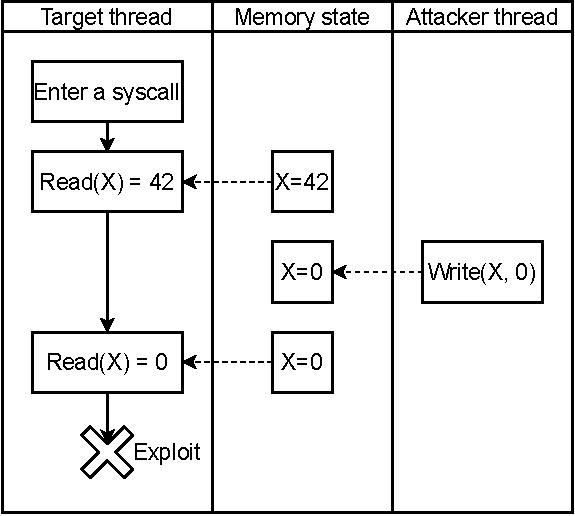
\includegraphics[width=.95\linewidth]{img/doublefetch.pdf}
  \caption{Example of a double-fetch bug.}
  \label{fig:doublefetch}
\end{figure}

Double-fetch bugs occur when a privileged environment (such as the kernel)
reads untrusted memory multiple times, returning different values each time.
Such a situation is depicted in \autoref{fig:doublefetch}, 
where the value of \Code{X} in memory is changed by an attacker
between two reads by the target thread.
Exploiting such a bug requires a race condition i.e. accesses 
to memory in a particular order across threads.
A specific variety is the \emph{time-of-check to time-of-use}~(\tocttou) 
bug which occurs when the first fetch validates an object's value and
the second fetch uses the same object's value.
\tocttou bugs are widely studied in file systems, where the
API makes it possible to swap the file after validating the access
rights~\cite{payer2012protecting,
pu2006methodical, wei2010modeling, tsafrir2008portably,Garfinkel03}.
\tocttou bugs affect both kernel~\cite{jurczyk2013bochspwn, wang2018survey}
and dynamically-loaded driver code~\cite{cve201812633,cve201812633fix}.
Wang et al.~\cite{wang2018survey} showed that double fetches appear not only
in kernels, but wherever there is a trust boundary to cross (e.g.,
kernel---hypervisor~\cite{wilhelm2016xenpwn} and hardware---kernel
boundaries~\cite{lu2018untrusted}).


%%%%%%%%%%%%%%%%%%%%%%%%%%%
%\section{Attack vectors}
%\label{sec:threats}
%%%%%%%%%%%%%%%%%%%%%%%%%%%

% In this section, we describe the threat model for exploiting double-fetch
% bugs in the kernel and classify the possible attacks based on how the
% data is modified between vulnerable double fetches.

\section{Threat Model}
\label{sec:threatmodel}
%%%%%%%%%%%%%%%%%%%%%%%%%

% Nothing fancy -- the adversary is just trying to hack the system
% No black magic allowed
The attacker has access to a user account on the target machine. They can
execute arbitrary userspace code, including syscalls. Some of the system
calls have double-fetch vulnerabilities which the attacker wishes to exploit
(e.g., for privilege escalation).
The attacker may execute arbitrary sequences of syscalls on multiple CPU
cores in parallel, or concurrently on the same core.

\midas mitigates any unintended corruption or information leakage \emph{in the kernel}
or \emph{in other user processes} that arises through double-fetch bugs.
Hardware attacks such as Rowhammer~\cite{mutlu2019rowhammer}
or side-channels~\cite{KocherHFGGHHLM019}, and file-system TOCTTOU
attacks~\cite{payer2012protecting, pu2006methodical, wei2010modeling,
tsafrir2008portably} are out of scope.


\section{Attack Classification}
\label{sec:attacks}
%%%%%%%%%%%%%%%%%%%%%%%%%%%%%%%%%%

\begin{table}
  \centering

    \begin{adjustbox}{width=1.0\linewidth}
    \begin{tabular}{  l | l | l | l }
  \toprule
      & \textbf{Userspace} & \textbf{Kernel} & \textbf{Device} \\ \midrule

      % Note: this is a manually tuned fixup. multirow just sucks.
      & Intra AS     & User mapping          & DMA       \\
      \multirow{-2}{*}{\shortstack[l]{\textbf{Existing} \\ \textbf{mapping}}}
      & Cross AS     & Kernel mapping        & MMIO page     \\
      \midrule

      & \Code{mmap}  & \Code{mm\_populate}   & New           \\
      & \Code{clone} &                       & DMA/     \\
      \multirow{-3}{*}{\shortstack[l]{\textbf{New} \\ \textbf{mapping}}}
      & \Code{swap}  &                       & MMIO page              \\
  \bottomrule
  \end{tabular}
  \end{adjustbox}
  \caption{Attack vector classification for \tocttou exploits.}
  \label{tab:attack_class}
\end{table}

\midas guards data processed during a syscall's execution against concurrent modification.
We label the data fetched twice as vulnerable data.
In this section, we classify attacks based on two criteria: the
privilege level of the writer, and whether the mapping used for writing
exists at the time of the first read. \autoref{tab:attack_class} summarizes our
classification.
Importantly, this classification helps understand existing attacks and how to
protect against them, and where future attacks (bugs) may arise.
The device column corresponds to attacks where a device
(e.g., a network card, GPU, FPGA) is responsible for modifying vulnerable data.
Watson~\cite{watson2007exploiting} describes a subset of the
following attack vectors.

Existing userspace mappings to a page can be used to modify
vulnerable data which the targeted syscall is reading.
Userspace can directly write to a mapped page, irrespective of whether the mapping is
in the same address space or not.
% Watson~\cite{watson2007exploiting} called such attacks
% \emph{direct double fetch} attacks.
Alternatively, a concurrently executing syscall can also modify the
vulnerable data in a \emph{confused-deputy} attack.
When the attacker passes a pointer to the vulnerable data to
the syscall as a user buffer in which the syscall can return some
data, the kernel's write to the buffer can modify vulnerable data.
For example, the \Code{read} syscall takes an argument pointing
to a user buffer where the contents of a file will be copied to.
Another example is \Code{rt_sigaction}, where the kernel writes to
a user buffer pointed to by the \Code{oldact} argument.
In both of these attacks, the malicious write uses a userspace
mapping.
\emph{A protection mechanism must account for all userspace
mappings to pages containing vulnerable data at the time of the
targeted syscall's first read.}

Existing kernel mappings to a page also mapped in userspace can be
leveraged by an attacker in a confused-deputy attack.
Here, the attacker maps a file-backed page from the page cache into a
userspace process and then passes as an argument in this page to the
target syscall.
The attacker then triggers a concurrent \Code{write} syscall to modify the
vulnerable data using kernel mappings for the page cache
pages.
% This attack is called \emph{inception double fetch}~\cite{watson2007exploiting}.
% \mat{Did we call it inception double fetch?}
The kernel does not explicitly track kernel addresses mapping to a page,
but the file-system driver does explicitly find the page before writing to it.
\emph{A protection mechanism must instrument file-system
drivers to account for writes via kernel mappings to vulnerable data.}

The kernel might create new mappings to the vulnerable data
between the double fetches by the target syscall, bypassing any 
protective permissions installed by the transfer function in 
PTEs at the time of first read.
An attacker can call \Code{mmap} and \Code{clone} to create
a new mapping to the vulnerable data before writing to it.
% The first version is called a \emph{reflected double fetch}
% attack~\cite{watson2007exploiting}.
The page-table mapping might not be created at the time of the malicious
syscall, but lazily when the attacker writes to the vulnerable data
due to demand paging.
In a more involved variant, the attacker can use the kernel as a
confused deputy which touches the unmapped page and maps it in,
then writes to the vulnerable data.
In all of the above vectors, the function populating pages for a
process (\Code{mm_populate} on Linux) is creating the new mapping.
\emph{A protection mechanism must instrument any syscalls
and other kernel mechanisms which can create new mappings.}

Swapping may also create a new page-mapping.
If the attacker writes to a page that was previously swapped
to disk, but later swapped in to be read by the target syscall in
a different address space, the kernel might lazily reinstate
the attacker's mapping to the page.
\emph{The swapping mechanism must be protected.}

\midas protects against all of the previously-listed attack vectors.
In the absence of any other syscall which can create new userspace
mappings to vulnerable data, \midas' protection is complete
against writes from both user and kernel code.

Finally, a device might modify vulnerable data if it is either
allowed to DMA (direct memory access) to the page, or if the page is memory 
mapped (MMIO) and is actually backed by the device.
In the latter case, external factors can change the vulnerable
data.
Existing discretionary access control rules typically prevent users
(except a superuser) from mapping device-backed pages into their
address spaces.
Such users are also disallowed from configuring DMA devices.
Thus, device modifications to vulnerable data fall outside
our threat model and are not protected by \midas.
% The superuser may load arbitrary kernel code % via loadable
% % modules
% and confused-deputy attacks leveraging an incompetent
% system administrator are also outside the purview of our threat model.
However, \midas can be extended to protect against modifications by DMA devices
on processors supporting IOMMUs or similar methods for
access control~\cite{olsonbordercontrol}.
As a superuser can modify kernel code via kernel modules, protecting against 
attacks from this user falls outside of our threat model.


%%%%%%%%%%%%%%%%%%%%%%%%%%%
\section{\midas Design}
\label{sec:design}
%%%%%%%%%%%%%%%%%%%%%%%%%%%

\midas maintains a single, core, \emph{invariant}:
\textbf{\emph{through a syscall's lifetime, every read to a userspace object
will return the same value}}.
By construction, the invariant guarantees that double-fetches in syscall
code will read the same data, \emph{eliminating \tocttou bugs}.
\midas maintains the invariant by tracking \emph{snapshots} of objects
when first accessed, lazily making \emph{copies} when the object is concurrently
written and accessing the correct copy on subsequent reads.
Copies are only maintained during syscalls' lifetimes, and are released as
soon as no syscall needs it.
Consequently, each userspace object has a single copy when no syscalls are
running.
The invariant also means that only accesses to userspace objects by the kernel
need to be protected.
Accesses to userspace objects from userspace and kernel objects by kernel
code remains unaffected.

\midas' implementation builds on the protection mechanisms provided by
existing virtual memory implementations.
On modern platforms, virtual memory protection is set up by the OS at
page granularity by setting bits in pagetable entries (PTEs).
These permission bits are checked by the hardware on memory access,
efficiently enforcing the permissions, and raising a fault when they
are violated.
For performance, \midas implements its invariant at page granularity, not object
granularity: when a syscall reads from userspace, every page touched by that
read is covered, not merely the bytes read.
Page-granularity protections are conservative compared to byte-granularity
protection and \midas maintains its invariant.
As a side-effect of its implementation, \midas does not distinguish
accesses to different parts of a page (intra-page false sharing).
False sharing leads to unnecessary page duplications, incurring performance
overhead on highly shared pages, but does not affect correctness.

For an object spanning multiple pages, \midas' design sequentially
protects each page before reading from it.
The leading pages containing the object are protected before the
later pages, allowing an attacker to potentially modify the later
pages before the syscall first reads them.
However, the attacker is prevented from modifying any of these pages
after the syscall's first read, ensuring that double fetches respect
the invariant.
If the syscall code contains a \tocttou bug, the modification will
be visible to the first fetch itself (which is used for checking for
validity of the data) and will lead to the data being rejected
straightaway.
\midas' invariant therefore prevent exploitation of double-fetch
vulnerabilities even when the fetched objects span multiple pages.
We elaborate on this case with an example in \autoref{sec:design:discussion}.

A major requirement for \midas is to allow concurrent access to pages
by user/kernel code running in parallel with a syscall which reads from
the same pages.
This requirement prevents deadlocks and improves performance \textit{vis-a-vis}
a na\"ive design which blocks all other tasks writing to pages already
read by a syscall until the syscall completes.
The na\"ive design can deadlock because it introduces dependencies between
tasks for forward progress, which we illustrate in the following example
of a system with two tasks (A and B):
\begin{inparaenum}[\itshape i\upshape)]
  \item Task A issues a blocking syscall which reads a user page and blocks, then
  \item Task B writes to the same user page before issuing a syscall which
  resumes task A.
\end{inparaenum}
In this case, if Task A's read to the page preceeds Task B's write,
Task B will be blocked waiting for A to complete its syscall.
Task A will also remain blocked waiting for Task B's syscall,
introducing a circular dependency, leading to deadlock.
The na\"ive design also introduces unnecessary delays in other cases,
such as the one described below, again with two tasks (C and D):
\begin{inparaenum}[\itshape i\upshape)]
  \item Task C reads from a page and sleeps for a long while,
        but does not read from the page a second time, then
  \item Task D writes to the same page after task C has read from it,
        and blocks until Task C completes and is unnecessarily delayed.
\end{inparaenum}
A more performant approach is to duplicate the concurrently accessed page:
the copy is kept for task C for future fetches, and task D
can write to the original and proceed without delays.

\midas must maintain multiple versions of a page read by a syscall
to maintain its invariant in the face of concurrent writes.
\midas introduces \emph{snapshots} and \emph{copies} to keep track
of page versions.
Snapshots are logical views of the page's contents at a particular time,
while the actual contents are stored in one of many copies.
Each snapshot maps to a copy, allowing the contents of the page at the
time of creating the snapshot to be read.
If multiple snapshots are taken without intervening writes to the page,
these snapshots will map to a single copy, reducing \midas' space overheads
and performance overheads for creating copies.
\midas maintains a snapshot of every page when first read by a syscall.
On a double fetch by the same syscall, the copy mapped to the snapshot
is accessed, ensuring that the data read is the same as the first time.
The latest copy of the page is used for all writes, by the syscall as
well as from concurrently running tasks, updating the page as seen
from userspace.
%
\midas' design draws parallels to multi-version concurrency control
methods for databases based on snapshot isolation~\cite{WuALXP17}.
Transactions read from a snapshot of the database state from when
they started, and writes update the up-to-date state of the database.
%
\emph{Essentially, \midas is a multi-versioning system for pages where
syscalls read from immutable versions to prevent \tocttou bugs and
syscalls and userspace both write to a single mutable version
holding the latest state of the page.}

\subsection{Page State Machine}

\begin{figure*}[]
  \centering
  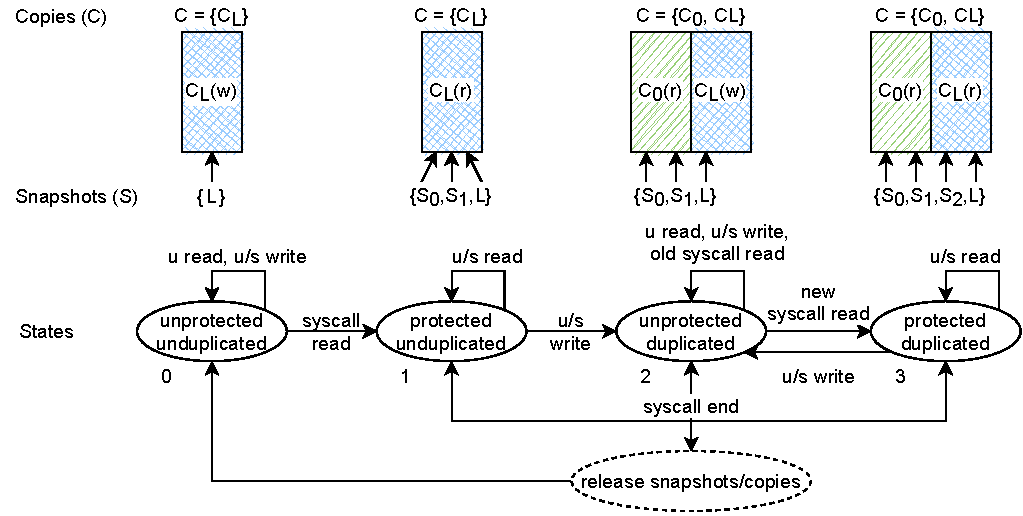
\includegraphics[width=0.9\linewidth]{img/midas_states.pdf}
  \caption{State diagram for a page in \midas. Reads/writes from userspace/syscall
          code are marked (u)/(s) respectively. Shading is used to represent the
          mapping from snapshots to copies.}
  \label{fig:midas_states}
\end{figure*}

\begin{figure}[h]
  \centering
  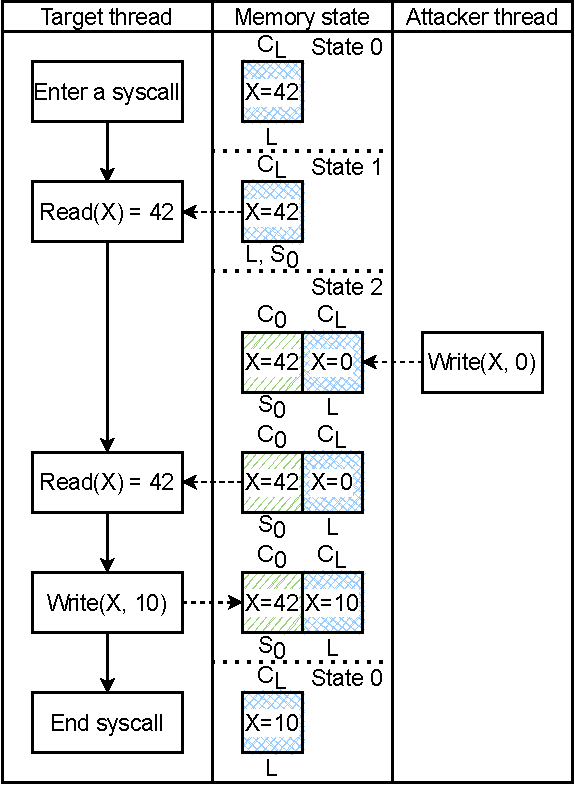
\includegraphics[width=0.95\linewidth]{img/doublefetch_midas.pdf}
  \caption{Diagram illustrating \midas preventing exploitation of a
  double fetch of object \Code{X}.}
  \label{fig:doublefetch_midas}
\end{figure}

To track multiple versions of the contents of a page when being concurrently
accessed by numerous tasks, from userspace or during a syscall,
\midas implicitly maintains a per-user page state machine.
For a page, its corresponding state machine
\begin{inparaenum}[\itshape i\upshape)]
  \item tracks snapshots for currently executing syscalls which have read it,
  \item tracks copies of the page, and
  \item maintains the mapping between snapshots and copies necessary for providing
  the correct contents to subsequent reads. % by these syscalls.
\end{inparaenum}

\autoref{fig:midas_states} shows the state machine for a single page.
At every state, the page has two associated sets:
\begin{inparaenum}[\itshape i\upshape)]
  \item the copies set $C = \{C_L, C_0, \dots\}$ holds multiple copies of the page over time, and
  \item the snapshots set $S = \{L, S_0, S_1, \dots\}$ tracks logical versions of the page, each corresponding to one executing syscall and each mapping to a copy.
\end{inparaenum}
Reads from kernel code in a syscall use the \emph{snapshot's corresponding copy}.
Writes from user/kernel code and reads from userspace access the \emph{latest
copy} $C_L$, which is mapped in processes' address spaces.
All other copies are read-only (no matter what the original page protection is), and are used for providing snapshots to syscalls.
Read-only pages only use states 0 and 1, and writes lead to segmentation faults
(as they do on non-\midas systems).
Knowing which state the page is in allows \midas to differentiate between
faults due to \midas protecting pages and faults due to actual permissions
violations in userspace programs or the kernel.
The latest copy $C_L$ of read-only pages remains read-only in both
protected states (1 and 3).
In the following paragraphs, we describe how the state machine for a single,
writable user page transitions between its states, what triggers each transition,
and what changes are made to the copies and snapshot sets on a transition.
In \autoref{fig:doublefetch_midas}, we illustrate how the state machine protects the
syscall from \autoref{fig:doublefetch}.

\paragraph{State 0}
A page starts as \texttt{(unprotected, unduplicated)}.
In this state, there is a single copy $C_L$ and a single ``snapshot'' $L$.
The snapshot $L$ refers to the latest version of the page which changes
over time, and is the only mutable snapshot.
All processes where this page is mapped have unrestricted userspace read and write
access, and unrestricted kernel write access.
The remaining operation, a read from kernel code, triggers a transition to
State 1.
In \autoref{fig:doublefetch_midas}, the snapshot $L$ initially contains
the value $42$.

\paragraph{State 1}
The page in State 0 transitions to the \texttt{(protected, unduplicated)} state as soon as a syscall
reads from it.
\midas first marks the page's latest copy $C_L$ read-only in all processes,
trapping writes to the page but allowing concurrent userspace reads to continue.
A new snapshot, $S_0$ linked to this syscall is allocated for this page.
For the rest of its lifetime, this syscall will only read this page from this snapshot.
Both snapshots $S_0$ and $L$ refer to the same copy $C_L$ (shown by the
blue cross-thatch in \autoref{fig:midas_states}).
Prior to any writes to this page, any other syscalls which also read the page
get their own snapshots (e.g., $S_1$) all pointing to the single copy $C_L$.
The page's read-only status causes the hardware to fault on any write,
notifying \midas to transition the page to State 2.
In \autoref{fig:doublefetch_midas}, the page transitions to State 1 when
the syscall first reads it, and adds a snapshot $S_0$.

\paragraph{State 2}
A page in State 1 transitions to the \texttt{(unprotected, duplicated)} state
on any write from user or kernel code.
\midas duplicates the old contents of the page from copy $C_L$, creating a
read-only copy $C_0$ (shown by green shading in \autoref{fig:midas_states}).
Snapshots except $L$ (i.e. $S_0$ and $S_1$) previously mapping to $C_L$ are
mapped to the copy $C_0$.
The write then modifies the latest copy $C_L$, which is made writable again.
Note how, in this state, any read using the snapshots $S_0$ or $S_1$ reads
from the unmodified copy $C_0$ while writes directly affect $C_L$.
Certain syscalls such as \Code{rt_sigaction} both read and write from
the same user page.
A write by \Code{rt_sigaction} to the page it has previously read will update
the page's latest copy $C_L$, but not the duplicate copy $C_0$.
\midas' write policy ensures that the copy $C_L$ always holds the latest
contents of the page, up-to-date with all the writes to the page, from both user
and kernel code.
Further, \midas does not need to merge writes from userspace and syscall code
on a syscall's completion, since both directly modify the same copy $C_L$.
All other copies $C_i$ are immutable.
When the attacker writes to the page in \autoref{fig:doublefetch_midas}, the
page moves to State 2, linking the snapshot $S_0$ to a copy holding the
original value $42$.
The writes from both the attacker and the syscall itself both affect
the copy $C_L$, but the read from the syscall accesses the snapshot $S_0$
and reads the same value as the first time.


\paragraph{State 3}
A separate syscall subsequently reading the page in State 2 transitions
it to the \texttt{(protected, duplicated)} state.
The new snapshot, $S_2$, points to the latest copy $C_L$.
State 3 is similar to State 1, except that there are different copies of
the page used for reading by different syscalls.
The syscall for which $S_0$ was allocated will read from the copy $C_0$,
while the syscall for which $S_2$ was allocated will read from copy $C_L$.
On a write, the page transitions to State 2 and is duplicated again,
creating another copy $C_1$: snapshot $S_2$ maps to $C_1$ while
snapshots $S_1$ and $S_0$ continue to map to $C_0$.

\paragraph{Releasing snapshots}
\midas uses snapshots to enable a syscall to read the same data from a page
during its lifetime and releases snapshots when syscalls complete.
Releasing a snapshot is possibly accompanied by a state transition
and the release of the mapped copy.
If $S_i$ mapped to the latest copy $C_L$, \midas cannot free the copy
since userspace is using it.
In this case, the page must be in State 1 or 3, and $C_L$ is read-only.
After removing $S_i$, if $L$ is the sole remaining snapshot mapped to $C_L$,
\midas makes the page writable, moving to State 0 or 2 from State
1 or 3 respectively.
If $S_i$ is mapped to any other duplicate $C_i$, \midas frees the copy along
with the snapshot if $S_i$ is the last remaining snapshot mapped to $C_i$.
If the page was in State 2, $C_L$ was writable and unmapped by any snapshot,
so \midas changes the page to State 0.
This transition is shown in \autoref{fig:doublefetch_midas}, where the
snapshot $S_0$ and the copy $C_0$ are both discarded.
If the page was in State 3, $C_L$ was read-only and mapped by some other
snapshot, so \midas moves the page to State 1.
Recall that all snapshots $S_i$ except $L$ are immutable.
Any data written by the syscalls directly affect $L$.
Therefore, dropping a snapshot $S_i$ is trivial and does not require
writes from the syscall to be merged into the latest copy.

\subsection{Discussion}
\label{sec:design:discussion}

\begin{table}
\begin{center}
  \begin{tabular}{  l  l }
  \toprule
    \textbf{System Call} & \textbf{Exemption reason} \\
  \midrule
    \Code{futex} & Relies on concurrent write \\
    \Code{execve} & Remaps address space \\
    \Code{write} & Invulnerable, improves performance \\
  \bottomrule
  \end{tabular}
\end{center}

\caption{System calls uninstrumented by \midas.}
\label{tab:except_syscall}
\end{table}

\paragraph{Correctness of syscalls directly updating snapshot $L$}
\midas' design lets all writes, including those from syscalls, to directly
update the latest copy of the page $C_L$ and this property maintains correctness
of system execution.
We now show that there is a valid, safe %\footnotemark
execution trace of a system not protected by \midas which generates the same
sequence of writes to the page, and therefore generates the same contents
of the page when the syscall ends.
%
We define a \emph{safe} trace as one that has no writes to vulnerable data between
double fetches by the kernel, and therefore does not trigger any existing
\tocttou bugs.
%
By showing that the final contents of memory after a \midas syscall has a
corresponding execution without \midas (which we assume to be correct)
leading to the same contents,
we can conclude that the execution of the \midas syscall is also correct.
For this proof, we assume that no syscall reads the same object after writing
to it (r-w-r pattern).
Such syscalls do not exist in the Linux kernel, and are discussed below.
Therefore, our syscalls write to an object after completing all of their reads
of that object.

% \footnotetext{A safe trace has no writes to vulnerable data between double fetches
% by the kernel, and therefore does not trigger any existing \tocttou bugs.}

Consider a page holding a single-byte object $O_0$, and the
sequence of operations to this byte during a \midas syscall be
$Ops = \{Op_0, Op_1, \dots \}$.
Each operation is a tuple $(r/w, k/u)$ specifying whether the
operation was a read or a write, and whether the operation was due to
a user or kernel instruction.
Suppose there was no attempt to exploit a \tocttou bug, i.e., between
any two read operations by the same syscall, there was no write to
this object.
% \mat{Second part of the conflict.}
% In case of the above mentioned scenario (1), which covers no concurrent
% writes, there are no writes to this object between any two read operations by
% the same syscall.
In this case, \midas reads the same value from its snapshot of the
object as is present on the latest version.
The same sequence of operations on a non-\midas system would be valid and
safe, since the object value does not change between the kernel's double
fetch and the syscall reads the same value on this system.

% \mat{Third part of the conflict.}
% Let us know focus on scenario (2) -- concurrent writes during a syscall's
% execution -- and
%
Assume there was an attempt to exploit a \tocttou bug:
a write $Op_1$ exists between two syscall reads $Op_0$ and $Op_2$.
\midas protects the syscall ensuring that $Op_2$ does not see the
effect of $Op_1$ by reading from a snapshot instead of the latest
copy $C_L$.
Since our syscalls are assumed to not contain any r-w-r pattern,
any writes by the syscall happen after $Op_2$.
Let us assume that the syscall's write is $Op_3$.
We can generate a valid, safe execution on a non-\midas system
by moving the attacker's write to after the last read by the
syscall, i.e., $Ops = \{Op_0, Op_2, Op_1, Op_3\}$.
The syscall in this system reads the same value both times, and
hence has the same execution as that in the \midas case.
The value of the object when the syscall completes is that
written by $Op_3$ in both cases (or that written by $Op_1$ when
the syscall does not have a final write).
Since the syscall has the same execution and the final value of
the object is the same, the execution of the \midas system
is the same as that of the non-\midas system.
In general, any trace of operations on a \midas system can
be translated  to a valid, safe trace on a non-\midas system
by moving malicious writes to an object to just after the last
double fetch of that object.
Multiple syscalls in \midas can therefore write to the same object
without affecting
correctness, because an equivalent, valid, safe non-\midas trace
exists where all of the writes have been postponed, in the same order
to after the double fetch reads.

\paragraph{Exemptions}
Syscalls such as \Code{futex} rely on user data changing between double
fetches to implement their functionality and cannot be protected by
\midas.
These syscalls are listed in \autoref{tab:except_syscall}.
The \Code{futex} syscall implements a fast synchronization mechanism
for userspace and relies on atomic writes from concurrent userspace
threads to update a condition the syscall is waiting for.
Subjecting a \Code{futex} syscall to \midas' invariant will prevent
it from ever waking up the waiting task.
Such syscalls cannot be protected by \midas, and we implement an
exemption list to prevent transitions in the state machines of pages read
by these syscalls.
The code for exempted syscalls must be manually inspected for double-fetch
vulnerabilities.
Crucially, exempting these syscalls from \midas' protection does not
affect the security of other syscalls containing double fetches.
Any writes from these syscalls are subject to the same rules described
in the state machine, and cannot break \midas' invariant.
\midas can also implement finer-grained exemptions based on syscall
parameters. Those were not necessary for Linux.
% Mat: the below is a bit stating the obvious, therefore commented.
%
% Other kernels may contain any number of
% syscalls which require exemption from \midas' protection, and
% they all need to be properly added to the exemption list.
% Finer grained exemptions based on syscall parameters can also be
% implemented, but was found unnecessary for Linux.
% A kernel where a majority of syscalls require exemption might not
% benefit from \midas' protection.


\paragraph{Syscalls with read-write-read patterns}
A (hypothetical) syscall that reads from an object, writes to it, and
then reads back the updated object cannot be protected using \midas.
\midas' invariant will ensure that the second read is identical to the first,
and does not reflect the intermediate write.
Such syscalls must remain exempt from \midas' instrumentation.
During extensive tests, we did not find any other syscall which exhibits this behavior in the Linux
kernel.

\paragraph{Syscalls with false sharing}
Another hypothetical type of syscall could struggle with \midas'
instrumentation due to false sharing.
Suppose a page contains two objects, $O_0$ and $O_1$, and a syscall
sequentially reads $O_0$ then $O_1$.
Due to \midas' invariant being enforced at page granularity and
false sharing of the page between these objects, \midas guarantees that
the value of object $O_1$ read is the same as what was contained when it
first read object $O_0$.
A syscall requiring the value of $O_1$ to change between these two
points in time would not work with \midas' protections.
Such a hypothetical syscall, requiring concurrent modifications to its
arguments, could exist to support some synchronization mechanism
similar to a \Code{futex} and can be safely exempt from \midas' invariant.
%
During extensive tests, we did not find any other syscall which exhibits this behavior in the
Linux kernel.


\begin{figure}[]
  \centering
  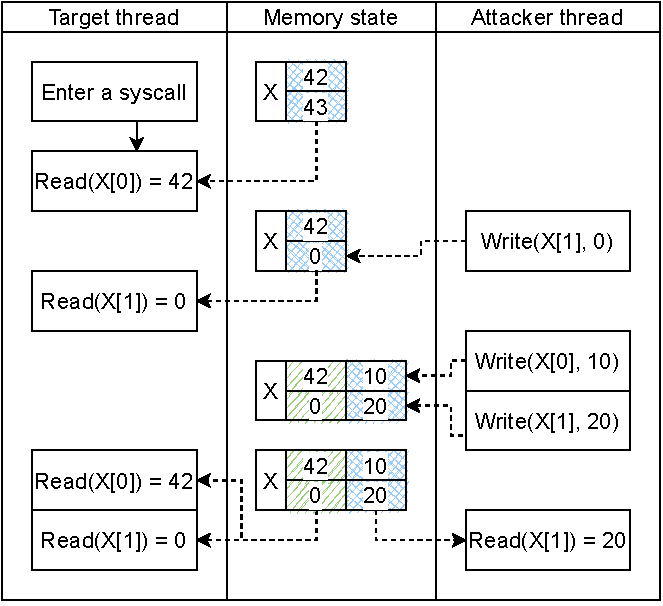
\includegraphics[width=\linewidth]{img/doublefetch_midas_twopages.pdf}
  \caption{Diagram illustrating \midas preventing exploitation
  of a double fetch of an object \Code{X} spanning two pages.}
  \label{fig:copy_two_pages}
\end{figure}

\paragraph{Example: Objects spanning multiple pages}
\autoref{fig:copy_two_pages} shows \midas protecting a syscall which
has a double fetch for an object spanning multiple pages.
Here, the two pages containing the object \Code{X} are accessed as
\Code{X[0]} and \Code{X[1]}.
The attacker tries to attack the syscall by changing the value of the
second page:
\begin{inparaenum}[\itshape i\upshape)]
\item between the syscall's first reads of \Code{X[0]} and \Code{X[1]}, and
\item between the first and second fetches of X.
\end{inparaenum}
\midas ensures both fetches return \Code{X=(42,0)}.
Critically, any existing TOCTTOU bugs are not triggered since both fetches
read the same, possibly invalid, value of the object.
Note how the situation is identical to one where the malicious write
to \Code{X[1]} happens before the syscall starts.

\paragraph{Preventing deadlocks by design}
\midas' design is free of deadlocks, and exempts syscalls which
require violation of its invariant from triggering particular
state-machine transitions.
Userspace reads always succeed, using the latest copy $C_L$ of the
accessed page.
Writes from userspace and kernel code succeed directly if the
page is in State 0 or 2, and trigger a fault otherwise.
Handling these faults involves creating a new copy of the page and
setting the page writable.
Reading from kernel code involves creating a new snapshot and
setting the page read-only.
None of the aforementioned operations relies on other operations
on the same page to complete and all are finite time.
None of the operations on a page rely on operations on other pages.
A single, per-page lock can serialize operations on that page
and assure forward progress.

\paragraph{Detecting double fetches}
\midas' state machine for pages enables the precise detection of double fetch
bugs, turning it into an effective sanitizer and developer debugging tool in
addition to being an efficient mitigation.
When a syscall first reads from a user page, it creates a snapshot
of that page.
On future reads, the snapshot is used in order to maintain the
invariant.
While reading from a page, implementations must check
if a snapshot exists for the syscall: if yes, the snapshot is used
for the read, otherwise a new snapshot is created and then used
for the read.
The existence of a snapshot means the syscall had previously
read from this page and had then created this snapshot, implying a double
fetch.
Unfortunately, this approach is prone to false positives due to false sharing.
The two reads might read from the same page, but access entirely
disjoint bytes.
\midas currently reports double fetches at page granularity.
A precise sanitizer could maintain a bitmask of accessed bytes to
prune false positives.


%%%%%%%%%%%%%%%%%%%%%%%%%%%%%%%%
\section{\midas Implementation}
\label{sec:impl}
%%%%%%%%%%%%%%%%%%%%%%%%%%%%%%%%

Our \midas prototype implements the state machine described in
\autoref{sec:design} on Linux version 5.11, targeting the x86-64
architecture.
A page protected by \midas transitions between states on
either a kernel read to user memory, or when user or kernel code
writes to protected, read-only memory (see \autoref{fig:midas_states}).
\midas can be implemented on any operating system kernel that
\begin{inparaenum}[\itshape i\upshape)]
\item systematically uses transfer functions for reading from userspace, and
\item on any architecture which implements hardware-controlled access
control to memory through page tables.
\end{inparaenum}
The first requirement enables \midas to implement transitions on
kernel reads from user memory.
The Linux kernel uses the \Code{raw_copy_from_user} interface which
we instrument for our prototype.
The second requirement causes the hardware to raise a fault on
writes to \midas-protected pages,
directing execution on the processor to a pre-defined exception
handler in the OS.
Our prototype instruments Linux' fault handler in the function
\Code{handle_pte_fault} to implement the write-triggered transmissions
from states 2 and 4.
Overall, our prototype adds around $1,100$ lines of code and modifies
17.
Our design allows the changes to be mostly limited to the memory
subsystem, and in general does not require individual syscalls to
be modified.
Only one syscall~(\Code{clone}) required code modification.

\subsection{Tracking Page State}
%%%%%%%%%%%%%%%%%%%%%%%%%%%%%%%%

\begin{figure}[]
  \centering
  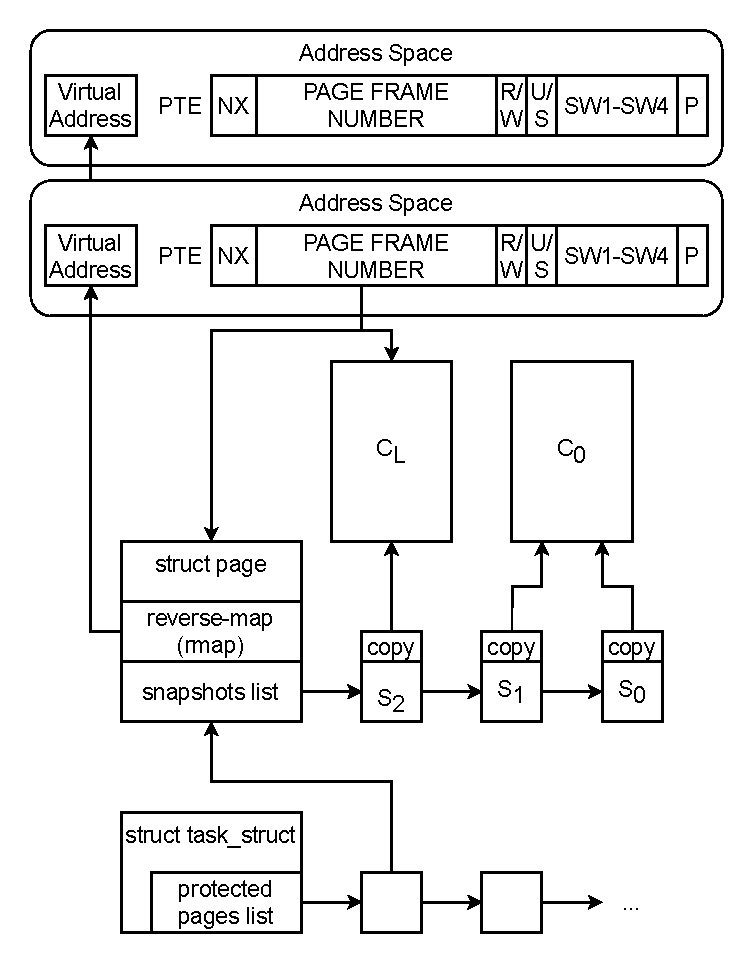
\includegraphics[width=\linewidth]{img/book-keeping.pdf}
  \caption{Bookkeeping information for a page.}
  \label{fig:midas_bookeeping}
\end{figure}

\midas needs to track the state for every userspace page, including
its snapshot and copy sets.
\autoref{fig:midas_bookeeping} shows the data structures used to
track a page's state in our prototype.
Linux maintains a \Code{struct page} object for every frame of
physical memory.
We augment \Code{struct page}  with a list holding the snapshots
for this page, excluding the latest snapshot $L$.
Each snapshot has a pointer to its copy.
In the figure, the snapshots $S_1$ and $S_0$ share the copy $C_0$.
We are aware of the strong aversion of the
Linux kernel developer community towards increasing the size of
\Code{struct page}.
An alternate implementation can use a hashmap to
map from a page's frame number to its snapshots list or
reuse existing data members (e.g., \Code{struct list_head lru} which
can be used as a generic list by page owners).

Each pagetable entry for a user page in different address spaces
maps the copy $C_L$, enabling userspace to directly access the page
with reads (and writes for writable pages).
We use one software-controlled bit (SW3) in the pagetable entries
to track the protection status of the page, and another
(SW2)\footnote{The SW2 bit is alternatively used by the experimental Software Dirty Pages feature of
Linux, and cannot be run alongside \midas in our prototype.}
to track the original protections for the page.
SW3 is set whenever the page is in one of the two protected
states (1 and 3).
On a write-triggered protection fault, SW3 can be read to
efficiently determine if the fault was due to \midas' protection
mechanisms, triggering a state change, or due to buggy software
accessing a page with illegal permissions, triggering a signal to
the task.
Other architectures might have fewer software-usable
bits in the page table, and implementations of \midas would
require storing the protection status of pages in a separate data structure.
The duplication status of the page is implicitly encoded in the
snapshots: the page is duplicated when any of its snapshots
holds a pointer to a copy other than $C_L$.

Changing a page's protection state requires PTE updates
in all address spaces where the page is mapped.
The page's \Code{struct page} structure includes a reverse-map
listing for all of these pages, and the corresponding virtual
address in each.
Our prototype uses this mapping to change PTE permissions across
all address spaces for a page.


\subsection{Kernel Reads from User Memory}
%%%%%%%%%%%%%%%%%%%%%%%%%%%%%%%%%%%%%%%%%%

\begin{figure}[]
  \centering
  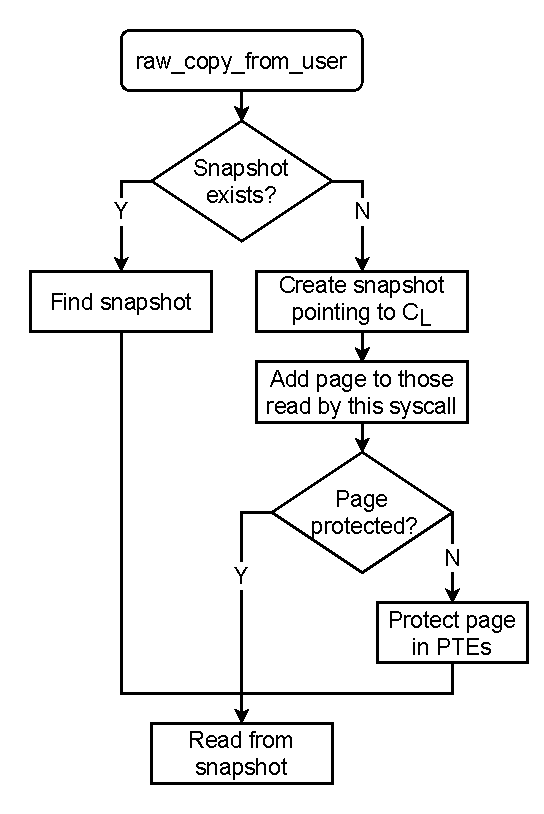
\includegraphics[width=0.8\linewidth]{img/copy_from_user.pdf}
  \caption{Flowchart for a syscall using the transfer function
          \Code{raw_copy_from_user}
          for reading from userspace.}
  \label{fig:copy_from_user}
\end{figure}

Syscalls reading from user memory the first time triggers the
allocation of a new snapshot.
If the page is not protected (states 1 and 3), the read also
triggers a state change where the kernel protects the page
in all address space that it is mapped in.
\autoref{fig:copy_from_user} shows the flowchart of the steps
implemented by the kernel function \Code{raw_copy_from_user} for
reading from user memory.
This function also uses the kernel's \Code{mark_page_accessed}
interface to move the page to the ``Active'' state for the
kernel's swapping mechanism, making the page ineligible for being
swapped out.
We also implement \Code{get_user} and \Code{unsafe_get_user}
(used by the kernel for small reads) as a call to \Code{raw_copy_from_user}.

\paragraph{Exemptions}
Our prototype \midas kernel exempts a couple of functions
from \midas' invariant (in addition to those described in
\autoref{sec:design:discussion}), and these functions are
therefore not instrumented
to follow the aforementioned steps while accessing userspace
memory.
First, \Code{raw_copy_from_user_inatomic} is a special
transfer function used by the kernel to
read user memory in special situations such as a kernel
oops\footnote{A kernel oops is triggered when the kernel detects a
problem while running which can affect its proper functioning, such
as corrupted data structures.
A more severe version, a kernel panic, causes the kernel to stop
executing, expecting data loss or damage if it does.}
where the kernel reads user memory to provide a backtrace.
In this severe situation, the kernel's goal is to collect debug
information before its imminent termination and no \tocttou protection
is needed.
Second, we also exempt the \Code{write} system
call's reads from user memory from instrumentation.
The \Code{write} syscall takes three arguments: a
file descriptor passed as a register, a pointer to a user
buffer and a count of bytes to be written to the file.
While the write to the file's pages is sensitive, and
\midas takes care to ensure that it follows the page state
machine, the read from userspace is not.
The syscall reads from userspace only once, and its data
is only used for copying into the file.
An attacker who modifies the user buffer concurrently with
the syscall only manages to change the contents written to
file, which it could have done anyway since it has access to
this buffer.
A kernel developer can similarly exempt other syscall which
they can prove to be secure from double-fetch bugs.


\subsection{Handling Faults}
%%%%%%%%%%%%%%%%%%%%%%%%%%%%

\begin{figure}[]
  \centering
  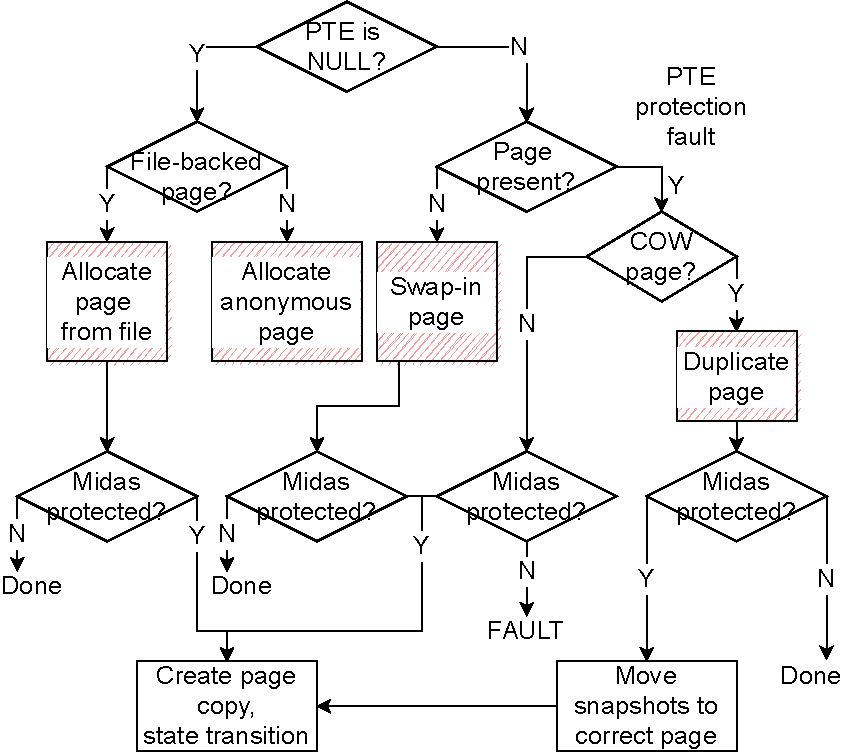
\includegraphics[width=\linewidth]{img/pagefault.pdf}
  \caption{Flowchart for handling a page fault. Shaded
          operations are unmodified.}
  \label{fig:fault_handling}
\end{figure}

\begin{figure}[]
  \centering
  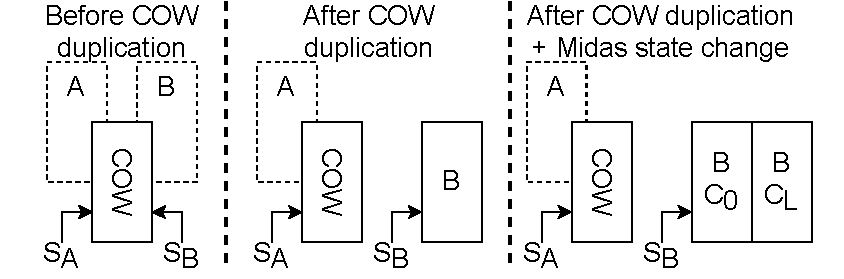
\includegraphics[width=\linewidth]{img/pagefault_cow.pdf}
  \caption{Flowchart for handling a page fault to a COW page.}
  \label{fig:fault_handling_cow}
\end{figure}

The memory management unit generates a fault when kernel or user code accesses
a page without having the correct permission in the corresponding PTE.
\midas marks writable pages read-only to protect them in
states 1 and 3, allowing the kernel to detect writes to these pages.
A common OS mechanism, copy-on-write (COW) pages, also uses
permissions in the PTE to detect when COW pages need to be copied.
The PTE's present bit are used to store pointers to file-backed pages
when they are swapped to disk.
\autoref{fig:fault_handling} shows the flowchart implemented by
\Code{handle_pte_fault} to handle faults for userspace addresses.

The page-fault handler first checks if the PTE is NULL, and if so
knows that it must allocate a page.
If the required page is anonymous, the page can be allocated as usual.
Otherwise, for file-backed pages, the handler has to check if the
page is already in a protected state (states 1 and 3) by reading
the SW3 bit of the PTE and if so, transitions to the required state
and allocates a new copy.
Pages in states 0 and 2 can be directly mapped, and subsequently
accessed.

For non-NULL PTEs, the handler checks if the PTE indicates that the
page is present.
Non-present pages need to be swapped in.
After finding the page, \midas then checks if the page was previously
swapped in by any other task and is now in a protected state.
For protected pages, \midas implements the required state change based
on whether the faulting access was a read or a write.

In the remaining case, faults for a present page indicate a
permission fault (for example, a write to a read-only page).
If the page is not a COW page, the handler then checks if the page
is in a protected state by checking the SW3 bit.
If the page was protected, a new copy is allocated and the page
transitions to the following state.
For non-protected pages, however, the fault implies a real access
violation, sending a signal to the process.

COW pages represent separate virtual pages from different
address spaces mapped to the same physical page.
An example of a COW page protected by \midas is shown in
\autoref{fig:fault_handling_cow}, where logically-separate pages A and B
are actually mapped to the COW page.
COW pages cannot be in states 2 or 3, since they cannot have multiple
\midas copies.
COW pages in state 0 can be dealt with by the kernel's standard
duplication method (not \midas' duplication).
For a COW page in state 1, its list of snapshots can correspond to
reads from syscalls for threads in different address spaces.
In \autoref{fig:fault_handling_cow}, we show snapshots $S_A$ and
$S_B$ corresponding to syscalls for threads in different address
spaces (containing A and B respectively).
These snapshots correspond to different logical pages, but are
all squashed into the snapshots list of the single COW page.
Therefore, after the kernel duplicates the COW page (new page
B created, in \autoref{fig:fault_handling_cow}), \midas moves
the snapshots for the faulting process ($S_B$) to the new page.
Here, \midas also updates the protected page list in the
affected syscalls' \Code{task_struct}s so that these structures
correctly refer to the new page.
Finally, the new page is transitioned to its next state to allow
for the write to occur, creating a new copy ($C_0$) for the
snapshot $S_B$ to read from.

We ensure that \midas' modifications to the fault handler
correctly handle concurrent faults and do not cause additional
nested faults.
During concurrent faults for the same page, only one thread
changes the page's state whereas the other directly uses the new
state.
The kernel's split page-table lock is reused to serialize state
changes.
We also ensure that the only additional accesses to user memory
within the handler (used for duplication) happen when the page
is assured to be in memory and correctly mapped.
All nested faults are therefore caused by existing kernel code
and do not interact with \midas' modifications.

\subsection{Syscall Completion}
%%%%%%%%%%%%%%%%%%%%%%%%%%%%%%%

On syscall completion, \midas cleans up snapshots allocated for
the syscall by instrumenting the end of \Code{do_syscall_64}.
\midas goes through the list of all the pages for which the
executing syscall has a snapshot, and frees those snapshots.
For snapshots which were the last to point to a copy, that
copy is also freed.


\subsection{File System Writes}
%%%%%%%%%%%%%%%%%%%%%%%%%%%%%%%

\midas instruments file-system writes to protect the kernel
from modifications via kernel mappings.
When a \Code{write} syscall writes to a file, it actually
writes to copies of pages of the file stored in memory within
a page cache.
In the spirit of abstraction, the kernel does not directly write to
these pages, but calls the relevant file-system (FS) driver instead.
The FS driver will access the page using kernel mappings when writing to pages in the page cache.
Since \midas only protects userspace mappings for protected pages,
writes by FS drivers will not raise a fault.
To comprehensively protect the page, any implementation needs to
instrument FS drivers' write functions.
Fortunately, FS drivers provided with the kernel follow a simple
recipe: for pages not in the page cache, the driver executes
FS-specific code to read the page into the page cache and then
call a generic function (\Code{generic_file_write_iter}) to actually
write the data into the page.
Instrumenting this generic function, therefore, protects the kernel
for a wide range of common file-systems (including ext4, nfs and
ntfs). \footnote{A more comprehensive list of kernel-provided FS drivers
protected via \Code{generic_file_write_iter} includes v9fs, ADFS, AFFS,
AFS, BFS, CIFS, eCryptfs, extFAT, ext2, F2FS,  FAT, FUSE, HFS, HFS+,
hostfs, HPFS, JFS, JFFS2, Minix, NILFS2, OMFS, OrangeFS, ramfs, ReiserFS,
SystemV, UBIFS, UDF, UFS, VboxSF, shmem.}
The added instrumentation checks whether the target page is
protected, and if so, transitions it to the next state and
creates a copy of the page before writing to the latest copy.

Our current prototype does not, however, protect out-of-tree drivers
which are not distributed with the kernel if they do not use the
\Code{generic_file_write_iter} function.
A user with superuser privileges can load a insecure module implementing a
FS driver which does not implement \midas checks.
A malicious superuser is, however, outside our threat model.
% Mat: IMO a very weak argument and always the case, so rather than waste
% precious time here, I've commented out the below as it distracts from our key
% argument IMO.
%
% A more reasonable threat involves a sysadmin unwittingly loading a
% insecure driver which a non-privileged user can then use to
% exploit a \tocttou bug.
% One solution would be for the kernel to inspect the relocations table of
% a new module while loading it to see if it uses \Code{generic_file_write_iter}
% and raising a warning if it does not.


\subsection{New Mappings to Protected Pages}
%%%%%%%%%%%%%%%%%%%%%%%%%%%%%%%%%%%%%%%%%%%%

Our \midas prototype preserves the state machine for user pages
across operations which create new mappings to a page to prevent
attacks which rely on mappings being created between double fetches.
The \Code{mmap} syscall is responsible for creating new virtual
memory mappings for processes, and requires instrumentation.
When \Code{mmap} is called with the \Code{MAP_POPULATE} flag, or
on the first access to the page, the \Code{mm_populate} function
is responsible for actually mapping the correct page in the
page table.
In our prototype, we check if the page being mapped is protected,
and if so, correctly protect the new mapping too.
Another syscall, \Code{clone}, duplicates a process' address space
when called without the \Code{CLONE_VM} flag, creating new mappings
to pages.
We instrument \Code{clone} to ensure that new mappings for protected
pages are also correctly protected.


\subsection{Discussion}
%%%%%%%%%%%%%%%%%%%%%%%

\paragraph{Optimizations on capable hardware}
To protect a page in an address space, a \midas implementation
needs to change the permissions in the page table for that page.
Modern CPUs cache virtual memory translations in per-core
Translation Lookaside Buffers (TLBs) which need to be (partially)
flushed on page-table updates (TLB shootdown).
On most CPUs, the core updating permissions will perform a global
shootdown to ensure that other TLBs for cores executing in the
same address space are also updated.
Implemented with inter-processor interrupts, global shootdowns
are expensive.
In our evaluation, 21\% of the runtime of the load generator
\Code{bombardier} used for stressing the Nginx server was spent
performing TLB shootdowns when running on the \midas kernel.

A more efficient solution would be to have special hardware support
for invalidating TLB entries globally, not just on the executing
core.
The AMD64 architecture manual~\cite{amd64prog} lists such an instruction
(\Code{INVLPGB}), though it is yet to be implemented in any commercially
available x86 processors.
The ARM v8-A architecture manual~\cite{armv8a} lists similar instructions
\Code{TLBI ASIDE1}\texttt{\textbf{IS}} and \Code{TLBI ASIDE1}\texttt{\textbf{OS}} which invalidate all PTEs
of a page within a cluster of cores but not for cores in other clusters
(Inner Shareable Domain) and cores across clusters (Outer
Shareable Domain) respectively.

Alternate architectures~\cite{0003BOBFP21midgard,ChaseLFL94SASOS} with a single,
system-wide translation table
would also benefit \midas by having a single page table to
update instead of multiple page tables for each address space a page
is mapped in.

\paragraph{Porting to other OSs}
\midas can provide \tocttou protection on other operating systems by
tracking the states of each page and implementing state transitions
as required.
OSs track page state in per-page state structures,
such as \Code{vm_state_t} for BSD-based OSs (*BSD) such as FreeBSD and XNU.
An implementation on these OSs must instrument the
read transfer function(\Code{copyin} for *BSD) to transition to states 1 and 3.
The OS' fault handler (\Code{vm_fault} on *BSD) will trap on writes to
protected pages, and needs to be modified to implement the required page
duplication and state change.

The remaining OS modifications for \midas support depends on
the OS' features.
If an OS allows userspace to map file pages, filesystem code to write
to these page needs to be modified.
Other syscalls which create/modify mappings to userspace pages will
also have to be instrumented to ensure that the new mapping respects the
page's state.
Such modifications are OS-specific, making it difficult to recommend
a generic methodology.


%%%%%%%%%%%%%%%%%%%%
\section{Evaluation}
%%%%%%%%%%%%%%%%%%%%

In this section, we emperically verify \midas' ability to mitigate
a known double fetch vulnerability, and quantify \midas' overhead on
workloads with different characteristics including both compute-bound
applications which rarely use syscalls and a mix of syscall-heavy applications
which heavily rely on the kernel's performance.

\subsection{Mitigation of CVE-2016-6516}
%%%%%%%%%%%%%%%%%%%%

\definecolor{mygreen}{RGB}{62, 123, 49}
% \begin{minipage}{\linewidth}
\begin{lstlisting}[language=C, escapeinside={<@}{@>},
                  basicstyle=\ttfamily, frame=single, numbers=left,
                  captionpos=b,
                  label=lst:cve-2016-6516,
                  caption={CVE-2016-6516: Vulnerable double fetch in \Code{ioctl_file_dedupe_range}.
                          Lines in green show the fix and testing code.},
                  float]
  //First fetch
  if(get_user(count,&argp->dest_count))
  {...}
  //Using first fetch
  size = offsetof(..., info[count]);
  //Secong fetch
  same = memdup_user(argp, size);
<@\texttt{\color{mygreen}{+ \textit{//Added check for bug}}}@>
<@\texttt{\color{mygreen}{+ \textbf{if}(same->dest\_count != count)}}@>
<@\texttt{\color{mygreen}{+ \ \ printk("Bug triggered");}}@>
<@\texttt{\color{mygreen}{+ \textit{// Fix: copy over original count}}}@>
<@\texttt{\color{mygreen}{+ same->dest\_count = count;}}@>
  //Using second fetch
  ret = vfs_dedupe_file_range(file,same);
\end{lstlisting}
% \end{minipage}

CVE-2016-6516 is a known vulnerability in kernels prior to version
4.7 in a file-system \Code{ioctl}.
The vulnerable code is shown in \autoref{lst:cve-2016-6516} and is
triggered when the value of the \Code{dest_count} object differs between
the two fetches (in lines 2 and 7).
\Code{memdup_user} uses the value from the first fetch for allocating a buffer
and copying in an array of descriptors from the user in line 7.
\Code{memdup_user} also contains the second fetch of \Code{dest_count}
which is later used in the function \Code{vfs_dedupe_file_range}.
An attacker who increases the size of \Code{dest_count} between the
two fetches will cause the kernel to access the copied array out-of-bounds,
causing a heap buffer overflow.

For verifying \midas' defense, we introduce a non-faulting assertion
check into the function~(lines 9--10) and run a known
exploit.\footnote{\url{https://github.com/wpengfei/CVE-2016-6516-exploit/tree/master/Scott\%20Bauer}}
The condition checks whether the fetched value of the user object (\Code{dest_count})
had changed, indicating a successful attack, and prints a message.
Finally, we re-introduce the fix for the bug (line 12), fixing the value of
\Code{dest_count} in \Code{same} to that from the first fetch.
In this setup, we can detect when the conditions for triggering the bug are met,
but also revert to a correct state allowing the kernel to safely
continue.
The exploit was able to successfully trigger the bug on the baseline kernel
every time over 10 runs.
With \midas enabled, the exploit was never triggered, i.e., both fetches
returned the same value on every call.\\


\subsection{Performance evaluation}
\label{sec:perf}
%%%%%%%%%%%%%%%%%%%%

We evaluate \midas on
\begin{inparaenum}[\itshape i\upshape)]
\item microbenchmarks targeting specific common syscalls,
\item workloads from two benchmark suites: the NAS Parallel
    Benchmark (NPB)~\cite{npb} and select workloads
    from the Phoronix Test Suite (PTS)~\cite{pts}, and
\item the webserver Nginx.
\end{inparaenum}
NPB includes compute-intensive multiprocessing workloads with a
low, but non-negligible syscall rate.
NPB therefore demonstrates the ability of \midas to
scale to systems where pages are protected across numerous
address spaces.
PTS includes a variety of benchmarks, both compute bound and
I/O bound representative of both desktop and server workloads.
PTS includes syscall-heavy applications with varying degrees
of parallelism.
The Nginx webserver is capable of both high request service rates
and scalability with multiple worker processes.
We do not include the SPEC CPU2017 benchmarks
as they are heavily compute bound and designed to isolate userspace
performance without syscalls, and are impervious to kernel performance.
SPEC benchmarks would unfairly bias performance in favor of
\midas.

The testbench for the evaluation consists of a desktop machine
with an 8-core Intel i7-9700 processor and 16GB DRAM running
Ubuntu 20.04 LTS. This configuration and CPU is commonly used on desktop
machines and workstations.
%
To eliminate the effect of dynamic frequency and voltage
scaling (DVFS), we set the processor to run at constant
frequency of 3.0GHz which is this model's base frequency.
In the \emph{baseline} configuration, we run the testbench
with the mainline kernel v5.11 available from Ubuntu's package
repository.
The \emph{\midas} configuration runs our prototype \midas kernel
also based on kernel v5.11.
For particular benchmarks, we also run the \emph{\midas{+}write}
configuration which also runs our prototype \midas kernel
but instruments all syscalls including \Code{write}.

\begin{figure*}[!t]
  \centering
  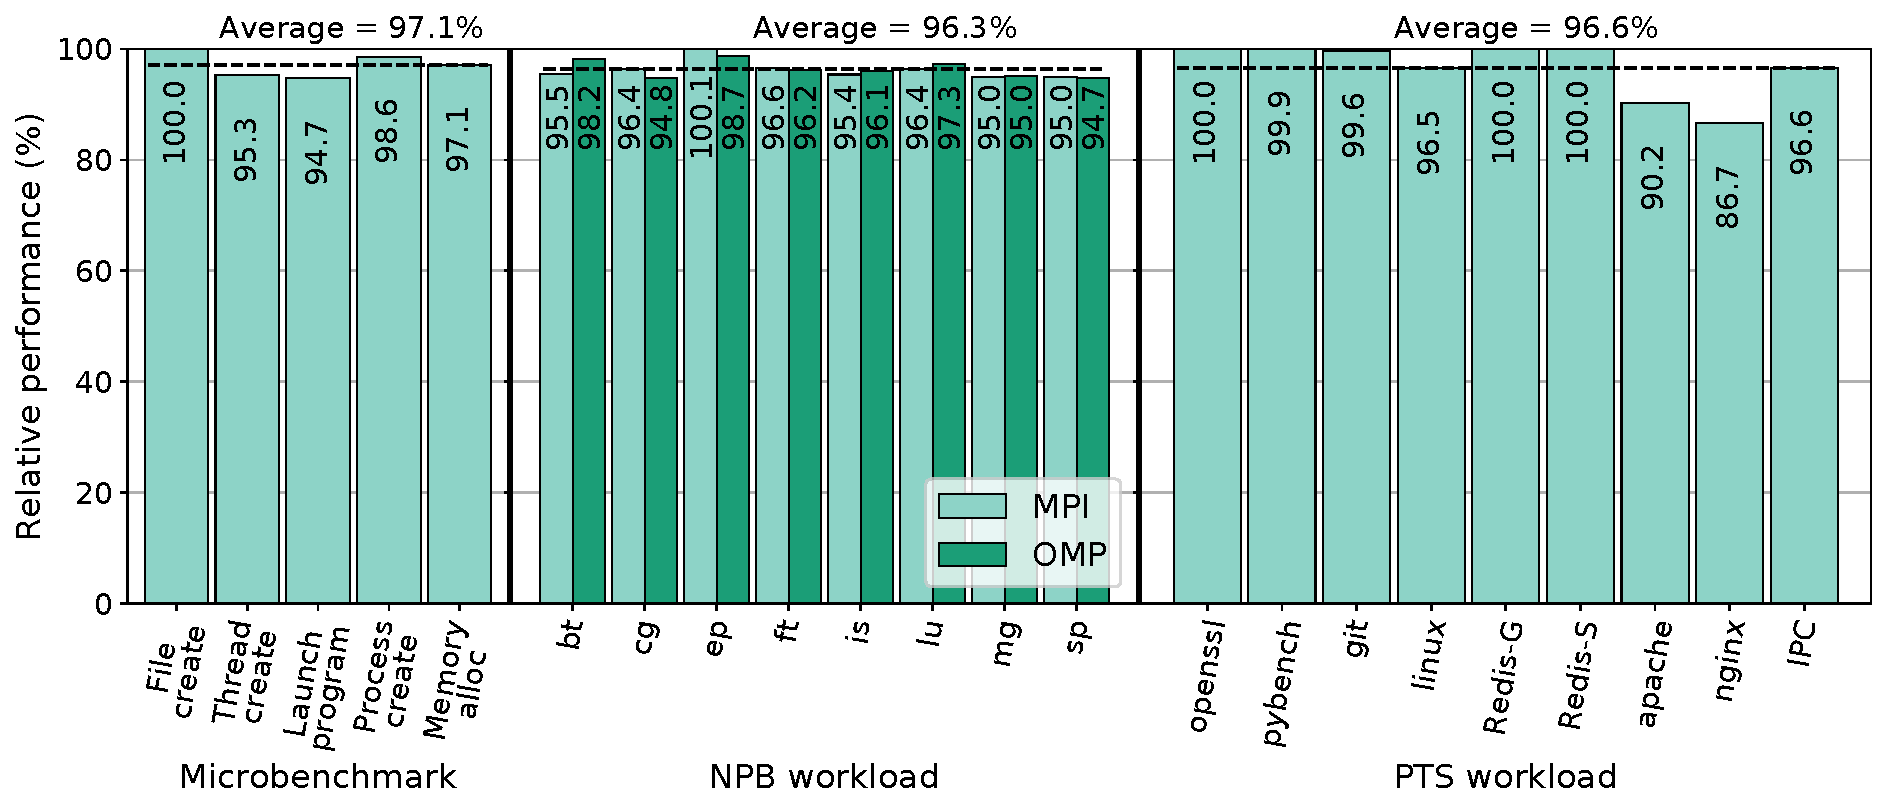
\includegraphics[width=\linewidth]{img/midas_performance.pdf}
  \caption{\midas' performance on microbenchmarks, NPB and PTS benchmarks
          relative to the baseline kernel.}
  \label{fig:midas_performance}
\end{figure*}

\begin{table}
  \centering
  \begin{tabular}{l l}
    \toprule
    \textbf{Microbenchmark} & \textbf{Top syscalls used} \\
    \midrule
    File creation & \Code{openat}, \Code{fstat}, \Code{write}, \Code{close} \\
    Thread/Process creation & \Code{mmap}, \Code{clone}, \Code{exit}, \Code{wait} \\
    Program launch & \Code{mmap}, \Code{execve}\Code{readlink}, \Code{openat} \\
    Mem alloc & \Code{brk} \\
    \bottomrule
  \end{tabular}
  \caption{Prominent syscalls used by OSBench microbenchmarks.}
  \label{tab:osbench_syscalls}
\end{table}

\paragraph{Microbenchmarks}
%%%%%%%%%%%%%%%%%%%%%%%%%%%%%%%%%%%%
We test \midas on microbenchmarks from
OSBench~\cite{osbench}.
The programs use \Code{libc} interfaces such as \Code{fopen},
\Code{pthread_create}, \Code{fork} and \Code{malloc} for creating files,
threads, processes and for memory allocation respectively.
\autoref{tab:osbench_syscalls} lists the prominent syscall usage
for these workloads.
\autoref{fig:midas_performance} shows \midas' performance
(time per operation)
on OSBench relative to the baseline kernel, with overheads ranging from
zero to 5.3\%.

\paragraph{NAS Parallel Benchmarks}
%%%%%%%%%%%%%%%%%%%%%%%%%%%%%%%%%%%%
NAS Parallel Benchmarks (NPB)~\cite{npb} is a benchmark introduced by
NASA.
NPB consists of several parallel programs using different communication
patterns and is available for two frameworks for parallel programming:
OpenMP and MPI.
OpenMP~\cite{dagum1998openmp} is a compiler extension that splits a
program's execution to multiple threads.
All threads still use the same address space, keeping the overhead minimal.
MPI~\cite{snir1998mpi} implements parallel execution by launching multiple
processes which communicate by message passing.
The two technology stacks have different frequency of syscalls due to
different communication methods.
Communication through kernel syscalls for either stack will incur overhead
due to \midas' protection.
Additional global TLB shootdowns (for snapshot synchronization) added by
\midas will also affect the performance of such parallel benchmarks.

We run NPB benchmarks of class A on our testbench, executing
4 threads or processes in parallel.
The benchmarks' runtime varies between 10 seconds and 8 minutes,
and are all long enough for the kernel to reach equilibrium.
Certain benchmarks require a parallelism number which is a perfect square.
On our 8-core CPU, having 4 compute-bound threads/processes instead of 16 allows
all threads to run without time sharing.
\autoref{fig:midas_performance} shows \midas' performance for both MPI and OpenMP,
normalized to the performance of the baseline system with the same parallelization
framework.
On average, \midas achieved $96.3\%$ of the baseline system's performance on
both frameworks.
\midas' performance for the \Code{ep} (Embarrassingly Parallel) benchmark is
closest to that of the baseline, since it has low communication overheads.
\midas shows low overhead ($3.7\%$) for compute-intensive, parallel workloads.


\paragraph{Phoronix Test Suite}
%%%%%%%%%%%%%%%%%%%%%%%%%%%%%%%%
The Phoronix Test Suite (PTS)~\cite{pts} includes a large set ($>500$) of
open-source benchmarks, of which we have chosen a range of benchmarks
suitable for evaluating both desktop and server performance.
We bias the selection to benchmarks that require (heavy) kernel activity to
test the overhead of \midas' instrumentation.
A sole benchmark, OpenSSL, is included to represent single-threaded,
compute-bound workloads for which kernel performance is less relevant.
The benchmarks are also varied, ranging from single-threaded (Pybench) to
multi-threaded, multi-process workloads (Apache).
At the extreme, we have an IPC benchmark transferring tiny, 128-byte
buffers between processes which spends all of its time in syscalls
and whose performance is entirely dependent on kernel IPC performance.

We plot \midas' performance relative to the baseline kernel on
these benchmarks in \autoref{fig:midas_performance}, roughly ordering
workloads in increasing order of syscall dependence from left to right.
For benchmarks for which PTS reports runtime, we compute the inverse
of the runtime as performance.
Benchmarks with low syscall frequency such as OpenSSL,
Pybench and Git have correspondingly low dependence on kernel performance.
Accordingly, these benchmarks see a negligible overhead when running
on our prototype kernel.
The benchmark titled ``Linux'' represents compilation of the Linux kernel.
While compilation is mostly compute bound, compiling the Linux kernel requires
accessing a large number of source files, resulting in the creation
of a large number of compiler processes each of which read and create
files.
\midas experiences a small, but non-negligible overhead of $3.5\%$ on this workload.
Redis requires syscalls for receiving and replying to requests, but
processes its transaction entirely in-memory.
Our evaluation prototype achieves practically identical results as the baseline,
highlighting the final prototype's competitive performance.
The webservers, Apache and Nginx require network and file-system I/O,
and rely heavily on syscall performance.
We see that Nginx, which is a higher-performance webserver, sees a larger
overhead.
IPC, which implements 128 byte transfers between
two processes over a TCP connection, is almost entirely bound by kernel
performance and sees a performance overhead of $3.4\%$ on \midas.

Our prototype \midas kernel benefits significantly from
exempting particular, proven-safe syscalls from instrumentation.
While we exclude \Code{write}-like syscalls from \midas because they
are not vulnerable to double-fetch bugs, we also evaluated the
performance cost of an unoptimized implementation (\midas{+}write)
which also instruments these syscalls.
To highlight the worst-case performance of the unoptimized implementation,
we evaluate the performance of the IPC benchmark on \midas{+}write due
to its high frequency of \Code{write} syscalls.
With \midas{+}write, the performance of the IPC benchmark falls to
$12.6\%$ of the baseline, a further degradation of $84\%$ compared
to \midas, showing that developer effort towards properly exempting
frequently called \emph{safe} syscalls from \midas protections is crucial
towards for implementations to maintain competitive performance
compared to the baseline.

\paragraph{Memory overhead}
Our prototype incurs memory overhead due to metadata, tracking page snapshots
and copies.
At any instant, the memory overhead mainly depends on the number of executing
syscalls (limited by the core count) and the number of page copies for these
syscalls.
On average, for every 1000 syscalls issued by the PTS benchmarks, our prototype
created 236 snapshots (32B each) and 54 copies (4KB each).
We can see that the occurrence of copies is low, resulting in negligible
memory overhead.

\subsection{Overhead breakdown}
%%%%%%%%%%%%%%%%%%%%

\begin{figure}
  \centering
  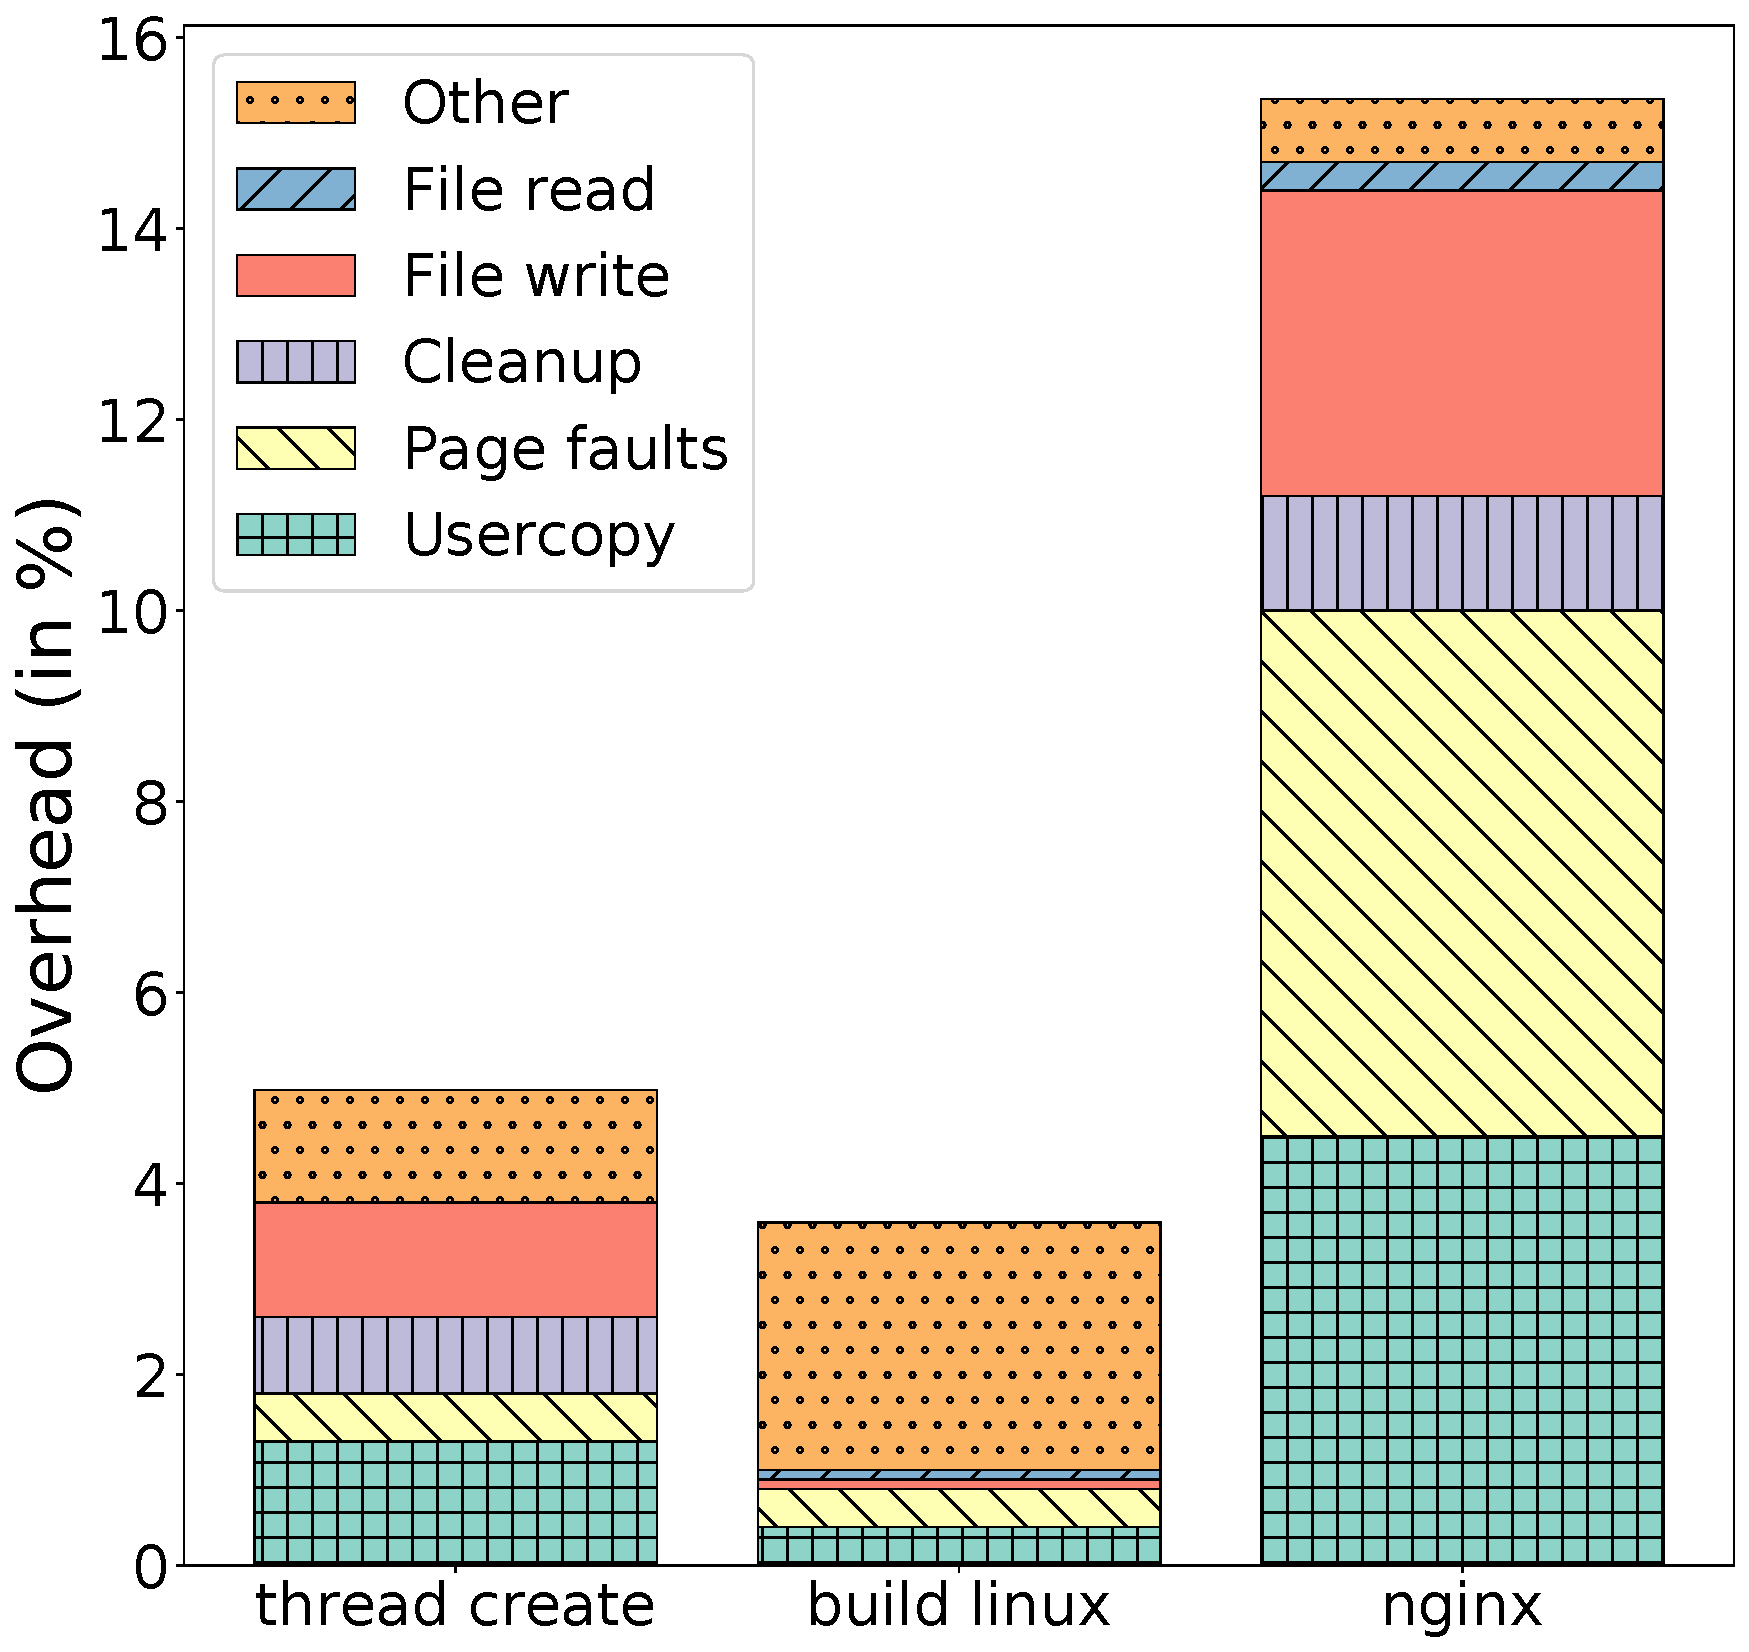
\includegraphics[width=\linewidth]{img/overhead.pdf}
  \caption{Classification of overheads for various benchmarks due to \midas.}
  \label{fig:overhead_class}
\end{figure}

In this section, we explore the sources of \midas' overhead by analyzing
\Code{perf} traces for three workloads: thread creation from OSBench, linux
compilation from PTS and Nginx.
We aim to classify overheads into the various kernel function we instrumented:
\begin{inparaenum}[\itshape i\upshape)]
\item user copy in transfer function,
\item page duplication on page fault,
\item metadata cleanup on syscall end, and
\item filesystem operations.
\end{inparaenum}

To estimate the time spent in each function, we create FlameGraphs for
each workload\cite{GreggFlameGraph} using samples of processor state, including
the call stack, collected over 30 second periods by \Code{perf record}.
After identifying one binary for the workload from the FlameGraph, we estimate
the overhead for a function as the difference in execution time attributed to
that function between the baseline and \midas systems.
The total overhead is estimated from the throughput figures obtained from
\autoref{sec:perf}.

\autoref{fig:overhead_class} shows the breakdown of overheads for three
workloads.
As expected, metadata tracking and duplication causes most overheads
for the user copy and fault handling functions respectively.
The results for the Linux build breakdown differs 
from the other workloads
in the large portion of
the unaccounted overhead (labelled ``Other'').
This anomaly stems for the fact that Linux's compilation runs a large number (1000s)
of processes, of which the compiler accounts for less than~50\% of the
total execution time.
The reported breakdown accounts for overheads on the compiler, but not
all the other processes.

Both page faults and user copies cause state changes for a page, and thereby
change the page's access permissions in the PTE.
The resulting TLB flush accounts for 0.3\%, 0\% and 1.1\% overhead for
thread creation, compilation, and Nginx respectively.
The load generator \Code{bombardier} used for loading Nginx, however, sees
a much larger overhead for TLB flushing, accounting for
21\% of its execution time.

\subsection{Case study: Nginx}
%%%%%%%%%%%%%%%%%%%%

\begin{figure}
  \centering
  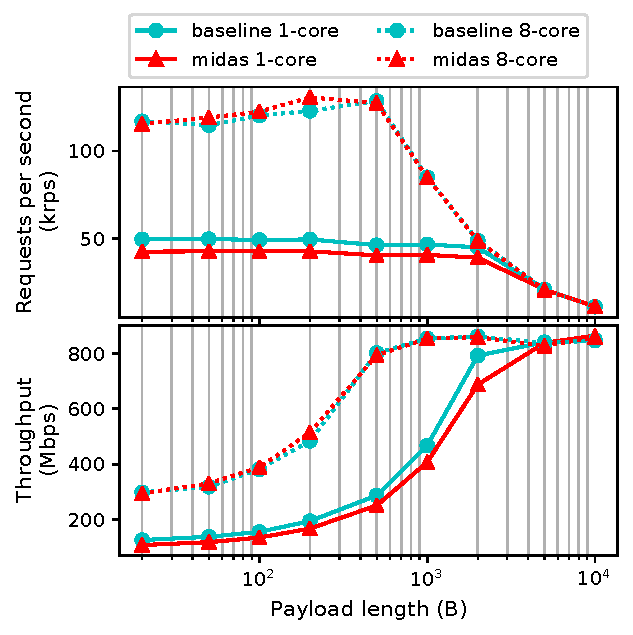
\includegraphics[width=\linewidth]{img/nginx_performance.pdf}
  \caption{Request rates and throughput served by the Nginx server for
          static pages.}
  \label{fig:nginx_perf}
\end{figure}

To better understand \midas' behavior under varying syscall
rates and different core configurations, we study Nginx's (version 1.18)
throughput while varying payload sizes and different worker counts.
Each worker is single threaded and uses one core.
The server is loaded with requests from a separate machine running
a load generater (\Code{bombardier}) with 100 concurrent
connections (chosen to maximize throughput) over a 1Gbps link.
The clients send http requests for files ranging between 20B and
10000B.

In \autoref{fig:nginx_perf}, we plot the request rate and throughput
for Nginx servers running with one and eight workers.
For all configurations, we can see that the rate of requests served
remains almost constant while increasing payload size until the network
link reaches saturation.
Under a saturated network, the request rates for \midas match that
of the baseline system.
With a single worker, \midas' overheads cause a consistent~13--14\%
overhead on the request rate for small packet sizes.
However, we see that \midas has practically no overhead when serving
requests with 8 workers even when packet sizes are too small to
saturate the network link.
In this case, both \midas and the baseline system are limited by the
scalability of the Linux networking stack.

%%%%%%%%%%%%%%%%%%%%
\section{Related Work}
%%%%%%%%%%%%%%%%%%%%

Early work on double-fetch bugs relied primarily on manual
code analysis to identify bugs in kernel code~\cite{YangCSS12, twizsgrakky07ring0}
or in syscall wrappers~\cite{watson2007exploiting}.
Realizing the limited scalability of this approach, particularly
when applied to large codebases such as the Linux kernel, subsequent 
work focussed on automated techniques based on static or dynamic 
analysis techniques, and on leveraging hardware features to mitigate
such bugs.

% Realizing that large projects such as the Linux kernel are not 
% amenable to extensive man
% In this section, we describe the automated tools that followed,
% based on static or dynamic analysis techniques, which can be employed
% to find and mitigate \tocttou bugs.

\paragraph{Static analysis}
%
Static analysis proposals use code analysis to find and fix double fetch
vulnerabilities.
DFTinker~\cite{dftinker} improves the coverage of pattern matching rules
for detecting double fetches in code as initially proposed by Wang~et~al.~\cite{wang2017double}.
Deadline~\cite{deadline} and DFTracker~\cite{wang2019dftracker} further
generalize the analysis by leveraging symbolic execution.

However, static analysis is severely limited by its requirement for
source code, which eliminates possibility of protecting of analyzing
binary-only modules for which code is not available.
In contrast, \midas can also protect such modules since well-behaving
module use the kernel transfer functions to access user memory.
Symbolic execution solves the generality problem of pattern-matching
approaches but has its limitations (path explosion, function pointers,
modelling numerous library functions, etc.).
Deadline~\cite{deadline} specifically requires the additional assumption
that pointer syscall argument do not alias, an assumption that can
wilfully be violated by our adversarial model.

Additionally, the protection allowed by static analysis methods are
limited: only the bugs which are detected can be fixed, and static
analyses are necessarily incomplete.
In contrast, \midas mitigates \emph{all} \tocttou vulnerabilities.
Further, specific cases of double fetches, such as in syscall wrappers
cannot be fixed in code, and require a versioning system such as
\midas in order to enable deep argument inspection.

\paragraph{Dynamic Analysis}
%
Dynamic analysis techniques leverage runtime information and values
to detect double fetches, and are notable in their ability to
find bugs in binaries.

To enable the search for various classes of bugs, Google Project Zero's
Bochspwn project~\cite{jurczyk2013bochspwn} introduced
a comprehensive emulator for \Code{x86} with callbacks to allow
tracing of kernel operations, including memory accesses.
When paired with a syscall fuzzer,
Bochspwn successfully detected and reported double fetches from
these access logs, but suffered from a high rate of false positives.
Another major shortcoming of Bochspwn was its low execution throughput
of 40-80MIPS which limited its ability to explore code paths.
Xenpwn~\cite{wilhelm2016xenpwn} extended Bochspwn's trace-driven 
approach to fuzz hypervisors for double-fetch bugs.
Xenpwn found three double fetches in the Xen hypervisor, but no critical 
vulnerabilities in KVM.

DECAF~\cite{schwartzDECAF} inverts \midas' adversarial model, leveraging
concurrent access to syscall parameters from userspace to detect kernel
accesses via a cache side-channel.
DECAF is strongly reliant on CPU-specific behavior, which
is sensitive to CPU parameters, subject to changes from generation to
generation (or even from core to core) and prone to noise and false sharing.
Following the discovery of transient-execution attacks~\cite{KocherHFGGHHLM019},
proposals such as InvisiSpec~\cite{YanCS0FT19,KhasawnehKSEPA19} have
tried to prevent
information leakage via cache side-channels.
Future generations might entirely close this channel, or introduce constraints
that limits this information flow.

Dynamic analysis techniques can only detect vulnerabilities on executed code
paths, and therefore typically rely on a fuzzer to extensively cover kernel code.
However, fuzzers are inherently incomplete, limiting the ability of dynamic
analysis to find bugs.

% PeriScope\cite{SongH0SNVVKSF19} is out of scope.
% Devices are outside the scope of the current implementation of \midas. Particularly, double fetches from device backed memory is liable to change without any control, but already requires high privileges which the user does not have. DMA accesses to main memory, however, can be protected by the use of IOMMUs with very low overhead [4], and can take advantage of the same \midas mechanisms. [4] Border Control: Sandboxing Accelerators.
% Overall comment: \midas does not seek to overthrow methods that seek to find double fetches, and fix them. In fact, it also allows use as a sanitizer that flags such double fetches. In the meanwhile, however, bugs do persist and are likely to persist in an environment incorporating third-party code in modules and a rapid pace of development. Here, \midas provides a strong, principled guarantee which is also future-proof.

\paragraph{Mitigations}
%
Previous attempts~\cite{schwartzDECAF,dftinker} to eliminate double fetch
vulnerabilities rely on Intel TSX, a hardware transactional
memory implementation, to detect malicious writes to data read by the
kernel.
A defense based on TSX improves upon \midas by reducing the scope for
false sharing from a page size to a cache size.
However, TSX suffers from major limitations which restrict its useability
for general kernel implementations.
Of note, TSX requires that the data working set for the critical section
experiences no L1 cache evictions, even due to contention from a
simultaneously-multithreaded (hyperthreading) core.
Further, TSX is limited to processors from a specific manufacturer (Intel),
leaving the vast majority
of computing devices~(mobile, IoT, AMD processors) unprotected.

%%%%%%%%%%%%%%%%%%%%
\section{Conclusion}
%%%%%%%%%%%%%%%%%%%%

\midas mitigates double-fetch bugs in system calls and protects the operating
system kernel by enforcing the invariant:  \emph{through a syscall's
lifetime, every read to a userspace object will return the same value}.
Our \midas implementation creates on-demand snapshots and copies of pages that
are read and merges any writes through the execution of the system call.
%
Our mitigation protects the core kernel, as well as drivers by carefully
instrumenting functions that interact with the process address space. While our
implementation focuses on Linux for x86-64, our concept is generic and empowers
other kernels to protect themselves against notoriously hard-to-find and
easy-to-exploit double fetch bugs.

The performance evaluation of our prototype implementation is promising.
Compute-bound benchmarks have negligible overhead and even syscall-intensive
benchmarks exhibit low overhead. On one hand, \midas mitigates all double fetch
bugs in the kernel and gives developers a tool to locate such bugs. On the other
hand, \midas sets the foundation for efficient, stateful system call filtering
and validation.
%
We have released the source code of our prototype as open-source at
\url{https://hexhive.epfl.ch/midas/}.
\end{namedscope}

%%%%%%%%%%%%%%%%%%%%%%%%%%%%%%%%
\appendices
%%%%%%%%%%%%%%%%%%%%%%%%%%%%%%%%

\begin{namedscope}{seccell}
\section{Formal Description and Analysis of \seccells' 
Userspace Instructions}
\label{app:instructions}

We define the semantics of \seccells' unprivileged instructions
in \autoref{fig:seccell_ops_formal} and discuss their corresponding
security checks below.

\paragraph{\sdswitch}
This instruction checks that the jump target is valid, and holds
an \sdentry instruction executable by the target \secdiv.
With the precondition that the caller \secdiv does not have
writable permission to any \cell executable by the target \secdiv,
\sdswitch guarantees compartment entry at previously defined entry 
points (helping implement call gates). 

\paragraph{\scprot}
This instruction checks that the target \cell is accessible by the
\secdiv, and the new permissions are a subset of the existing permissions.
After this instruction, the \secdiv is assured to have no more permissions
than before.

\paragraph{\scgrant, \screcv and \sctfer}
\scgrant checks that the granting \secdiv has permissions to the
\cell, and that the granted permissions are a subset of its existing
permissions.
\screcv, in turn, checks that the \secdiv is receiving permissions for a
valid cell, that the permissions were previously granted by the
specific \secdiv that the receiving \secdiv expects, and that the received
permissions are a subset of the permissions granted.
\sctfer includes the checks of both \scgrant and \scprot.
The granting and receiving \secdiv{}s must cooperate in order to
transfer permissions, and together finish with the same or fewer
permissions than they began with.

A correct compartment is defined to not grant or receive any permissions 
or invalidate cells that it is not required to grant as per a correct
compartmentalization policy.
Considering a set of compromised attacker \secdiv{}s and their permissions 
to \cell{}s and assuming that uncompromised compartments are correct,
\seccells guarantees that the attackers can neither gain any new permissions 
through any sequence of permission transfer instructions 
nor elevate the permissions of any uncompromised compartment.
Using \scgrant and \screcv instructions, the compromised compartments can
transfer permissions between themselves but those grants cannot include 
permissions which none of the attackers had initially.
The only way for the attackers to gain permissions is from
an uncompromised \secdiv either granting permissions to a \cell or from 
invalidating a private \cell which one of the attackers can validate with \screval.
The only way for the attackers to inject permissions is to have an
uncompromised \secdiv receive them.
By definition, uncompromised compartments will do neither of the above.
Once again, we stress on the importance of a correct compartmentalization
policy.
No mechanism, including \seccells, can protect against an insecure policy
where compartments transfer permissions from/to untrusted compartments
without proper validation.

\paragraph{\scinval} 
This instruction allows a \secdiv to invalidate a \cell to which
it has exclusive access, and to which no outstanding permission grants
exist.
The first condition can be true for a private region, or for one
which other \secdiv{}s have willingly dropped permissions.
Consequently, no other \secdiv will unwittingly lose permissions to
the invalidated \cell as a consequence of \scinval.
The second condition provides the assurance that no compartment can
regain permissions to the cell without executing \screval.

\paragraph{\screval} 
This instruction checks that the address corresponds to an existing 
\cell{} and that it is currently invalid. 
Due to the initial invalidity of the \cell, no \secdiv{}s could have
access to the cell to be revalidated.

\paragraph{\scexcl}
This instruction does not modify any permissions, only allowing a
\secdiv{} to check if it has exclusive access to a \cell{} to which
it already has access to.

\begin{comment}
\section{Memory layout of the unified \ptable-\gtable}
\label{app:ptable}

\autoref{fig:ptable_layout} shows the detailed implementation of the
unified \ptable-\gtable.

The table contains a sorted list of cell descriptors, including a
metadata ``cell'' used for storing its sizing parameters.
As described in \autoref{sec:impl}, each cell descriptor stores virtual 
and physical frame numbers uniquely identifying a VMA, as well as a 
validity flag to track the cell's current validity.
The metadata cell tracks the number of allocated \cell{}s ($N$), the
number of \secdiv{}s ($M$), and sizing factors $T$ (upper bound on \cell count)
and $R$ (upper bound on \secdiv count).
When software requires additional \secdiv{}s or \cell{}s, it must request
the supervisor via a system call.
If the request overflows the bounds imposed by factors $R$ and $T$, the
supervisor must resize this table as required.
The \cell descriptor list is followed by the \ptable, and then by the
\gtable.

\atri{Show how the limits on number of cells and secdivs is determined}

\begin{figure*}
  \centering
  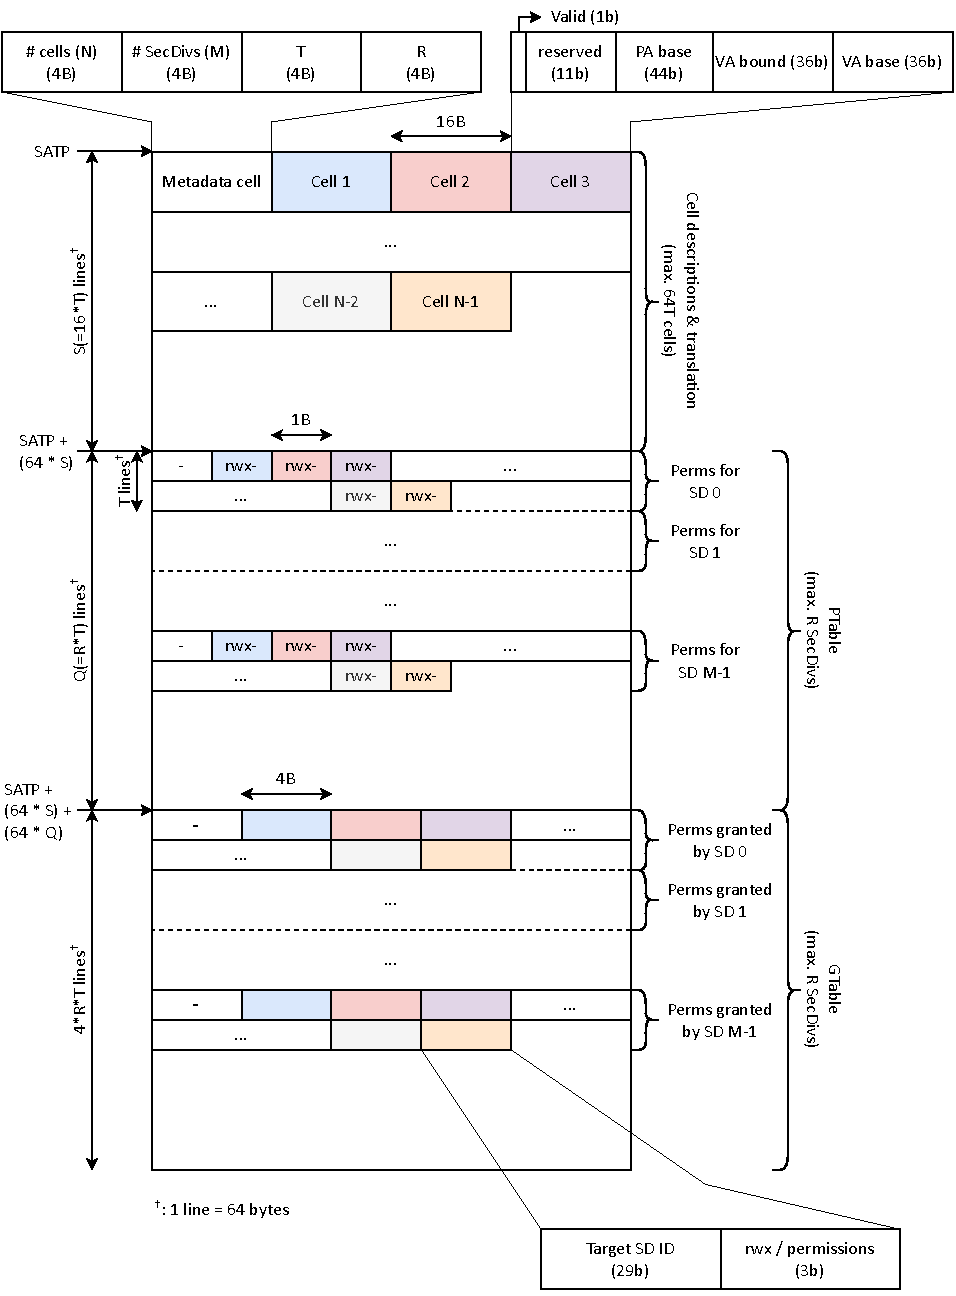
\includegraphics[height=0.95\textheight]{media/seccells/ptable_layout.pdf}
  \caption{Layout of the unified \ptable-\gtable.}
  \label{fig:ptable_layout}
  %\Description[<short description>]{<long description>}
\end{figure*}
\end{comment}

\section{Justification for \autoref{tab:req_comparison}}
\label{app:justification_table1}

\paragraph{Obj. \req{1a}}
MPK, ERIM and Donky do not check permissions for instruction fetches, 
simplifying code injection.
Under our threat model, an attacker can inject \Code{wrpkru} instructions 
to corrupt permissions.

\paragraph{Obj. \req{1b}}
Through code injection, call gates in MPK and ERIM can be bypassed.

\paragraph{Obj. \req{1c}}
CODOM requires migrating threads without context isolation.
MPK, ERIM and Donky rely on call gates if context isolation is desired.
However, MPK and ERIM cannot enforce call gates under our threat model.
Donky gives no mechanism for a compartment to restore its state without
trusting general-purpose registers. 
Further, Donky cannot adopt a \seccells-like software approach because a 
compartment has no way to identify itself.

\paragraph{Obj. \req{1d}}
CHERI allows one compartment to unilaterally send a capability to another compartment, 
unchecked by the TCB and unacknowledged by the receiver.

\paragraph{Obj. \req{1e}}
No mechanism except XPC considers the challenge of exclusive access.

\paragraph{Obj. \req{1f}}
A compartment in MPK and ERIM cannot check the value of the \Code{pkru}
register for another compartment, hindering audits.
Cross-core \Code{pkru} reads are not possible.
CHERI requires an expensive full memory scan for capabilities to perform
an audit.

\paragraph{Obj. \req{2a}}
Page-table based translation and permission checking encounter TLB-reach
limits leading to multi-cycle common case access verification for many
widely-used programs including \Code{memcached}. The mechanisms relying on
such page tables for either translation or permission checking fail this
requirement.

\paragraph{Obj. \req{2b}}
Supervisor-mediated cross-compartment calls in UNIX-like OSs,
Mondrian, lwC and CHERI require 100s or 1000s of cycles to complete.

\paragraph{Obj. \req{2c}}
Supervisor-mediated permission transfers are slow (UNIX, MMP, lwC).
MMP proposes the use of redundant mappings with different permissions
to implement a form of zero-copy transfer which is not generic.
CODOM does not really support permission transfers.
XPC restricts permission transfer to a single relay segment.

\paragraph{Obj. \req{3a}}
CODOM identifies the executing compartment by the instruction pointer, 
limiting the flexibility to share code/data regions between compartments.

\paragraph{Obj. \req{3b}}
UNIX, MMP, lwC, XPC and CHERI cannot eliminate context switching when a
permissive policy allows migrating threading between compartments.

\section{Existing mechanisms with \seccells}
\label{app:integrate_exist}
Many existing performance or security mechanisms can be integrated with
\seccells, either unmodified or with modifications described in this section.

\paragraph{Physical Memory Protections}
\seccells enforces permissions on the virtual address space, and is therefore
trivially compatible with physical memory protection schemes 
including RISC-V's Physical Memory Protection (PMP) mechanism, 
processor reserved memory for Intel's SGX
and vendor-specific protections like Qualcomm's XPU~\cite{qualcomm_ac}.
These mechanisms will apply to the physical address output by 
\seccells' MMU after \ptable access control checks.

\paragraph{Pointer authentication and capabilities}
ARM's pointer authentication code (PAC) feature and CHERI's capabilities
improve memory safety by protecting pointers from illegal 
modifications (overwriting when stored in memory and out-of-bound
increment respectively). Both mechanisms are orthogonal to,
and can integrate with \seccells, which checks accessess against \ptable
permissions when the 
pointers protected by these mechanisms are finally dereferenced, providing
another layer of protection against attacks like PACMAN~\cite{pacmanRavichandranNLY22}.

\paragraph{Hardware and Software Control Flow Integrity}
Hardware (e.g., Intel CET) and software (e.g., LLVM-CFI) control-flow
protections can integrate with \seccells, 
improving intra-compartment control-flow protection to
complement \seccells' inter-compartment call gates (\sdentry).
CET can continue to check indirect call targets for \Code{endbr} instructions. 
LLVM's and other fine-grained CFI pointer checks are implemented in software, 
orthogonal to hardware control flow checks.


\paragraph{Page-based mechanisms}
By itself, \seccells restricts popular mechanisms (e.g., guard pages, swapping)
operating on pages and page tables since translations and protections are 
tracked at \cell granularity.
However, \seccells can be integrated with upcoming intermediate address-space 
systems like Midgard re-enabling programmers to implement these crucial 
features.
Midgard couples \seccells-like range-based translation at the core with
a second level of page-granularity translations at the backside of the 
last-level cache.
Guard pages and swapping can both be implemented by unmapping the requisite pages 
in the backside translation.


\section{Speculative Side-Channel Attacks}
\label{app:sidechannel}

We consider the threat of speculative side-channel attacks like 
Spectre~\cite{KocherHFGGHHLM019}
in \seccells' design, despite omitting such attacks from our attacker model.
\seccells{} introduces additional mechanisms for changing an executing
thread's permissions, through userspace compartment switching and
permission transfers.
Fault-based attacks like Meltdown~\cite{lipp18sec} must be prevented in
implementations by preventing faulting loads from accessing memory or
forwarding their data to subsequent instructions~\cite{WeisseNLWK19}.

\seccells specifies that userspace instructions are serializing, 
precluding speculative permission changes.
An attacker cannot, for example, speculatively switch to a victim
\secdiv using an \sdswitch following a long-latency branch and read 
the victim's private data using the victim's permissions.
\seccells' permission transfer instructions are atomic, preventing visibility 
or exploitation of any intermediate permission state.
An attacker \secdiv cannot, for example, drop permissions for a \cell
using \scprot while transferring the same permissions using \sctfer in parallel.
Our firmware (and future microcode) implementation use load-linked 
store-conditional atomic operations commonly available across architectures
to ensure atomicity.
\seccells allows the pipeline to speculate as usual within a compartment's 
execution, and speculative accesses are also subject to access control 
by the MMU and cannot illegally access any \cell.
Access control, therefore, also limits the leakage potential of existing
Spectre gadgets.
Whereas a Spectre gadget on a traditional processor can address and
access any user memory in the process' address space, the same Spectre
gadget can only access memory within the compartment's \cell{}s.
\seccells also limits the code (speculatively) executable within a compartment,
further restricting the availability of Spectre gadgets.

\section{\seccells Implementation Trade-Offs}
\label{app:impl_options}

\seccells permits a range of implementations scaling from simple 
microcontrollers with firmware emulation for added userspace
instructions to server grade processors with microcode or hardware 
implementations. In this section, we describe the trade-offs and 
justify our implementation in \autoref{sec:impl}.

\paragraph{Firmware}
On the simplest side of the spectrum, instructions can be emulated
by firmware using trap-and-emulate.
Firmware is programmable code which runs in a privileged execution mode 
and uses native ISA instructions.
\seccells' instructions will trap into firmware, and be dispatched to 
the emulation code.
Firmware implementations are cheap, requiring no additional hardware, but 
slower than alternate implementations.
For the simple RISC-V RocketChip microcontroller, we choose 
firmware emulation for permission transfer instructions.
Note that the firmware can also forward traps to be emulated by
either the supervisor or even a privileged userspace library.
However, the additional security risk of emulation by less trusted
software risk and the overhead of forwarding traps makes such
implementations less attractive.

\paragraph{Hardware}
Alternatively, instructions can be implemented in hardware with 
finite-state machine circuits.
While this design option implies better performance,
designing complex hardware comes with silicon and power costs and
substantial complexity.
Hardware bug fixes incur the significant cost of the tape-out process.
Server and desktop processors generally include beefy cores with
large silicon area, where hardware implementations may match the
processor's targeted performance.
We implement the crucial \sdswitch instruction in hardware
to reap the performance advantage,
and because of the simplicity of its design.

\paragraph{Microcode}
A third option, microcode, is programmable code provided by the 
processor manufacturer, built from low level operations including ones 
not available through the ISA interface.
When a instruction implemented in microcode is encountered, a microcode
sequencer fetches microcode from an on-chip RAM and executes them in the
pipeline.
Microcode eliminates the cost of trapping and dispatch encountered in 
firmware emulation ($77\%$ of the latency of emulating \scprot),
and can also leverage hardware-specific optimizations.
Microcode is popular for implementing complicated instructions
with high performance like SGX's \Code{EENTER}/\Code{EEXIT} instructions.
Microcode also has the advantage of being programmable, and have been
leveraged to fix processor errata and bugs.
While the simple RocketChip lacks a microcode sequencer, 
we envision microcode to be ideal for implementing \seccells'
permission transfer instructions for high-performance processors.
\end{namedscope}


%-------------------------------------------------------------------------------
\backmatter

\bibliographystyle{IEEEtran}
\phantomsection
\addcontentsline{toc}{chapter}{Bibliography}
\bibliography{thesis}


\end{document}